\title{函数（2016--2025 高考真题）}
\author{}
\date{}
\maketitle
\noindent 本专题共 154 道题，按年份排列。每题标注原卷与原题号。

\section*{2016 年}

\begin{question}[points=5]
\textbf{来源：}2016 年 全国III卷-理科，第 6 题\par
已知 $a=2^{\frac{4}{3}}$, $b=4^{\frac{2}{5}}$, $c=25^{\frac{1}{3}}$, 则
\begin{choices}
  \item $b<a<c$
  \item $a<b<c$
  \item $b<c<a$
  \item $c<a<b$
\end{choices}
\begin{solution}
\textbf{答案：}$b<a<c$

\textbf{分析：}$b=4^{\frac{2}{5}}=2^{\frac{4}{5}}$, $c=25^{\frac{1}{3}}=5^{\frac{2}{3}}$, 结合幂函数的单调性可比较 $a,b,c$.

\textbf{详解：}$a=2^{\frac{4}{3}}=2^{\frac{20}{15}}$, $b=4^{\frac{2}{5}}=2^{\frac{4}{5}}=2^{\frac{12}{15}}$, $c=25^{\frac{1}{3}}=5^{\frac{2}{3}}=5^{\frac{10}{15}}$, 由于 $2^{\frac{12}{15}}<2^{\frac{20}{15}}<5^{\frac{10}{15}}$, 即 $b<a<c$, 故选 A.
\end{solution}
\end{question}

\begin{question}[points=5]
\textbf{来源：}2016 年 全国III卷-文科，第 7 题\par
已知 $a=2^{\frac{4}{3}}$, $b=4^{\frac{2}{5}}$, $c=25^{\frac{1}{3}}$, 则 ( )
\begin{choices}
  \item $b<a<c$
  \item $a<b<c$
  \item $b<c<a$
  \item $c<a<b$
\end{choices}
\begin{solution}
\textbf{答案：}$b<a<c$

\textbf{分析：}$b=4^{\frac{2}{5}}=(2^2)^{\frac{2}{5}}=2^{\frac{4}{5}}$, $c=25^{\frac{1}{3}}=(5^2)^{\frac{1}{3}}=5^{\frac{2}{3}}$, 结合幂函数的单调性, 可比较 $a,b,c$.

\textbf{详解：}$a=2^{\frac{4}{3}}$, $b=2^{\frac{4}{5}}$, $c=5^{\frac{2}{3}}$, 由幂函数 $y=x^{\frac{4}{3}}$ 在 $(0,+\infty)$ 上递增, 得 $2^{\frac{4}{5}}<2^{\frac{4}{3}}<3^{\frac{4}{3}}$, 又 $3^{\frac{4}{3}}=(3^4)^{\frac{1}{3}}=81^{\frac{1}{3}}$, $c=5^{\frac{2}{3}}=(5^2)^{\frac{1}{3}}=25^{\frac{1}{3}}$, 因为 $81>25$, 所以 $3^{\frac{4}{3}}>c$, 故 $b<a<c$. 故选 A.
\end{solution}
\end{question}

\begin{question}[points=5]
\textbf{来源：}2016 年 全国II卷-理科，第 12 题\par
已知函数$f(x)$（$x\in\mathbb{R}$）满足$f(-x)=2-f(x)$，若函数$y=\frac{x+1}{x}$与$y=f(x)$图象的交点为$(x_1,y_1)$，$(x_2,y_2)$，$\ldots$，$(x_m,y_m)$，则$\sum_{i=1}^{m}(x_i+y_i)=$（\quad）
\begin{choices}
  \item $0$
  \item $m$
  \item $2m$
  \item $4m$
\end{choices}
\begin{solution}
\textbf{答案：}$m$

\textbf{分析：}由条件可得$f(x)+f(-x)=2$，即有$f(x)$关于点$(0,1)$对称，又函数$y=\frac{x+1}{x}=1+\frac{1}{x}$的图象关于点$(0,1)$对称，即有$(x_i,y_i)$为交点，即有$(-x_i,2-y_i)$也为交点，计算即可得到所求和．

\textbf{详解：}两个函数图象都关于点$(0,1)$对称，故交点成对出现，每对关于点$(0,1)$对称，设$m$为奇数时中间交点为$(0,1)$，则$\sum (x_i+y_i)=m$．故选B．
\end{solution}
\end{question}

\begin{question}[points=5]
\textbf{来源：}2016 年 全国II卷-文科，第 10 题\par
下列函数中，其定义域和值域分别与函数$y=10^{\lg x}$的定义域和值域相同的是
\begin{choices}
  \item $y=x$
  \item $y=\lg x$
  \item $y=2^x$
  \item $y=\frac{1}{\sqrt{x}}$
\end{choices}
\begin{solution}
\textbf{答案：}$y=\frac{1}{\sqrt{x}}$

\textbf{分析：}$y=10^{\lg x}$定义域和值域均为$(0,+\infty)$。$y=\frac{1}{\sqrt{x}}$定义域和值域均为$(0,+\infty)$，相同。
\end{solution}
\end{question}

\begin{question}[points=5]
\textbf{来源：}2016 年 全国II卷-文科，第 12 题\par
已知函数$f(x)(x\in\mathbf{R})$满足$f(x)=f(2-x)$，若函数$y=|x^2-2x-3|$与$y=f(x)$图象的交点为$(x_1,y_1)$，$(x_2,y_2)$，…，$(x_m,y_m)$，则$\sum_{i=1}^m x_i=$
\begin{choices}
  \item $0$
  \item $m$
  \item $2m$
  \item $4m$
\end{choices}
\begin{solution}
\textbf{答案：}$m$

\textbf{分析：}函数$f(x)$关于$x=1$对称，$y=|x^2-2x-3|$也关于$x=1$对称，故交点关于$x=1$对称，$\sum x_i = \frac{m}{2}\times2=m$。
\end{solution}
\end{question}

\begin{question}[points=5]
\textbf{来源：}2016 年 全国I卷-理科，第 7 题\par
函数$y=2x^2-e^{|x|}$在$[-2,2]$的图象大致为（ ）

\begin{center}
  
\includegraphics[width=.42\linewidth]{assets/asset-006-01.jpg}
\end{center}
\begin{choices}
  \item A图像
  \item B图像
  \item C图像
  \item D图像
\end{choices}
\begin{solution}
\textbf{答案：}D

\textbf{分析：}根据已知中函数的解析式，分析函数的奇偶性，最大值及单调性，利用排除法，可得答案．

\textbf{详解：}解：因为$f(x)=y=2x^2-e^{|x|}$，所以$f(-x)=2(-x)^2-e^{|-x|}=2x^2-e^{|x|}$，故函数为偶函数，当$x=\pm2$时，$y=8-e^2\in(0,1)$，故排除$A$，$B$；当$x\in[0,2]$时，$f(x)=y=2x^2-e^x$，所以$f'(x)=4x-e^x=0$有解，故函数$y=2x^2-e^{|x|}$在$[0,2]$不是单调的，故排除$C$，故选：$D$．
\end{solution}
\end{question}

\begin{question}[points=5]
\textbf{来源：}2016 年 全国I卷-理科，第 8 题\par
若$a>b>1$，$0<c<1$，则（ ）
\begin{choices}
  \item $a^c<b^c$
  \item $ab^c<ba^c$
  \item $a\log_b c<b\log_a c$
  \item $\log_a c<\log_b c$
\end{choices}
\begin{solution}
\textbf{答案：}C

\textbf{分析：}根据已知中$a>b>1$，$0<c<1$，结合对数函数和幂函数的单调性，分析各个结论的真假，可得答案．

\textbf{详解：}解：因为$a>b>1$，$0<c<1$，所以函数$f(x)=x^c$在$(0,+\infty)$上为增函数，故$a^c>b^c$，故$A$错误；函数$f(x)=x^{c-1}$在$(0,+\infty)$上为减函数，故$a^{c-1}<b^{c-1}$，故$ba^c<ab^c$，即$ab^c>ba^c$；故$B$错误；$\log_a c<0$，且$\log_b c<0$，$\log_a b<1$，即$\frac{\log_a c}{\log_b c}=\log_a b<1$，即$\log_a c>\log_b c$．故$D$错误；$0<-\log_a c<-\log_b c$，故$-b\log_a c<-a\log_b c$，即$b\log_a c>a\log_b c$，即$a\log_b c<b\log_a c$，故$C$正确；故选：$C$．
\end{solution}
\end{question}

\begin{question}[points=5]
\textbf{来源：}2016 年 全国I卷-文科，第 8 题\par
若$a>b>0$，$0<c<1$，则
\begin{choices}
  \item $\log_ac<\log_bc$
  \item $\log_ca<\log_cb$
  \item $a^c<b^c$
  \item $c^a>c^b$
\end{choices}
\begin{solution}
\textbf{答案：}$\log_ca<\log_cb$

\textbf{分析：}根据指数函数，对数函数，幂函数的单调性结合换底公式，逐一分析四个结论的真假，可得答案。

\textbf{详解：}$\because a>b>0$，$0<c<1$，$\therefore \log_ca<\log_cb$，故$B$正确；$\therefore$当$a>b>1$时，$0>\log_ac>\log_bc$，故$A$错误；$a^c>b^c$，故$C$错误；$c^a<c^b$，故$D$错误。故选：$B$。
\end{solution}
\end{question}

\begin{question}[points=5]
\textbf{来源：}2016 年 全国I卷-文科，第 9 题\par
函数$y=2x^2-e^{|x|}$在$[-2,2]$的图象大致为
\begin{choices}
\end{choices}
\begin{solution}
\textbf{答案：}$D$

\textbf{分析：}根据已知中函数的解析式，分析函数的奇偶性，最大值及单调性，利用排除法，可得答案。

\textbf{详解：}$\because f(x)=y=2x^2-e^{|x|}$，$\therefore f(-x)=2(-x)^2-e^{|-x|}=2x^2-e^{|x|}$，故函数为偶函数，当$x=\pm2$时，$y=8-e^2\in(0,1)$，故排除$A$，$B$；当$x\in[0,2]$时，$f(x)=y=2x^2-e^x$，$\therefore f'(x)=4x-e^x=0$有解，故函数$y=2x^2-e^{|x|}$在$[0,2]$不是单调的，故排除$C$，故选：$D$。
\end{solution}
\end{question}

\section*{2017 年}

\begin{question}[points=5]
\textbf{来源：}2017 年 全国III卷-理科，第 15 题\par
设函数$f(x)=\begin{cases} x+1, & x\le 0 \\ 2^x, & x>0 \end{cases}$，则满足$f(x)+f(x-\frac{1}{2})>1$的$x$的取值范围是．
\fillin[{$(-\frac{1}{4},+\infty)$}]
\begin{solution}
\textbf{答案：}$(-\frac{1}{4},+\infty)$

\textbf{分析：}根据分段函数的表达式，分别讨论$x$的取值范围，进行求解即可。

\textbf{详解：}若$x\le 0$，则$x-\frac{1}{2}\le -\frac{1}{2}$，则$f(x)+f(x-\frac{1}{2})>1$等价为$x+1+x-\frac{1}{2}+1>1$，即$2x>-\frac{1}{2}$，则$x>-\frac{1}{4}$，此时$-\frac{1}{4}<x\le 0$。当$x>0$时，$f(x)=2^x>1$，$x-\frac{1}{2}>-\frac{1}{2}$，当$x-\frac{1}{2}>0$即$x>\frac{1}{2}$时，满足$f(x)+f(x-\frac{1}{2})>1$恒成立。当$0\ge x-\frac{1}{2}>-\frac{1}{2}$，即$\frac{1}{2}\ge x>0$时，$f(x-\frac{1}{2})=x-\frac{1}{2}+1=x+\frac{1}{2}$，此时$f(x)+f(x-\frac{1}{2})>1$恒成立。综上$x>-\frac{1}{4}$。故答案为：$(-\frac{1}{4},+\infty)$。
\end{solution}
\end{question}

\begin{question}[points=5]
\textbf{来源：}2017 年 全国III卷-文科，第 7 题\par
函数$y=1+x+\frac{\sin x}{x}$的部分图象大致为（       ）

\begin{center}
  
\includegraphics[width=.42\linewidth]{assets/asset-011-01.jpg}
\end{center}
\begin{choices}
  \item A．
  \item B．
  \item C．
  \item D．
\end{choices}
\begin{solution}
\textbf{答案：}D

\textbf{分析：}通过函数的解析式，利用函数的奇偶性的性质，函数的图象经过的特殊点判断函数的图象即可。

\textbf{详解：}函数$y=1+x+\frac{\sin x}{x}$，$f(x)=x+\frac{\sin x}{x}$是奇函数，图象关于原点对称，则$y=1+x+\frac{\sin x}{x}$的图象关于$(0,1)$对称，当$x\to 0^+$时$f(x)>0$，排除A、C；当$x=\pi$时$y=1+\pi$，排除B。
\end{solution}
\end{question}

\begin{question}[points=5]
\textbf{来源：}2017 年 全国III卷-文科，第 12 题\par
已知函数$f(x)=x^2-2x+a(e^{x-1}+e^{-x+1})$有唯一零点，则$a=$（          ）
\begin{choices}
  \item A．$-\frac{1}{2}$
  \item B．$\frac{1}{3}$
  \item C．$\frac{1}{2}$
  \item D．$1$
\end{choices}
\begin{solution}
\textbf{答案：}C

\textbf{分析：}通过转化可知问题等价于函数$y=1-(x-1)^2$的图象与$y=a(e^{x-1}+e^{-x+1})$的图象只有一个交点。分$a=0,a<0,a>0$三种情况讨论。

\textbf{详解：}当$a>0$时，$y=1-(x-1)^2$最高点$A(1,1)$，$y=a(e^{x-1}+e^{-x+1})$最低点$B(1,2a)$，要唯一零点需$A,B$重合，即$2a=1$，$a=\frac{1}{2}$。
\end{solution}
\end{question}

\begin{question}[points=5]
\textbf{来源：}2017 年 全国III卷-文科，第 16 题\par
设函数$f(x)=\begin{cases} x+1,&x\le 0 \\ 2^x,&x>0 \end{cases}$，则满足$f(x)+f(x-\frac{1}{2})>1$的$x$的取值范围是           。
\fillin[{$(-\frac{1}{4},+\infty)$}]
\begin{solution}
\textbf{答案：}$(-\frac{1}{4},+\infty)$

\textbf{分析：}根据分段函数的表达式，分别讨论$x$的取值范围，进行求解即可。

\textbf{详解：}当$x\le 0$时，$f(x)+f(x-\frac{1}{2})=x+1+x-\frac{1}{2}+1=2x+\frac{3}{2}>1$，解得$x>-\frac{1}{4}$，此时$-\frac{1}{4}<x\le 0$；当$x>0$时，$f(x)=2^x>1$，则$f(x)+f(x-\frac{1}{2})>1$恒成立。综上$x>-\frac{1}{4}$。
\end{solution}
\end{question}

\begin{question}[points=5]
\textbf{来源：}2017 年 全国II卷-文科，第 8 题\par
函数 $f(x)=\ln(x^2-2x-8)$ 的单调递增区间是
\begin{choices}
  \item $(-\infty,-2)$
  \item $(-\infty,-1)$
  \item $(1,+\infty)$
  \item $(4,+\infty)$
\end{choices}
\begin{solution}
\textbf{答案：}$(4,+\infty)$

\textbf{分析：}由 $x^2-2x-8>0$ 得: $x\in(-\infty,-2)\cup(4,+\infty)$, 令 $t=x^2-2x-8$, 则 $y=\ln t$, 结合复合函数单调性“同增异减”的原则, 可得答案.

\textbf{详解：}由 $x^2-2x-8>0$ 得: $x\in(-\infty,-2)\cup(4,+\infty)$, 令 $t=x^2-2x-8$, 则 $y=\ln t$, $\because x\in(-\infty,-2)$ 时, $t=x^2-2x-8$ 为减函数; $x\in(4,+\infty)$ 时, $t=x^2-2x-8$ 为增函数; $y=\ln t$ 为增函数, 故函数 $f(x)=\ln(x^2-2x-8)$ 的单调递增区间是 $(4,+\infty)$. 故选D.
\end{solution}
\end{question}

\begin{question}[points=5]
\textbf{来源：}2017 年 全国II卷-文科，第 14 题\par
已知函数 $f(x)$ 是定义在 $\mathbb{R}$ 上的奇函数, 当 $x\in(-\infty,0)$ 时, $f(x)=2x^3+x^2$, 则 $f(2)=$
\fillin[{$12$}]
\begin{solution}
\textbf{答案：}$12$

\textbf{分析：}由已知中当 $x\in(-\infty,0)$ 时, $f(x)=2x^3+x^2$, 先求出 $f(-2)$, 进而根据奇函数的性质, 可得答案.

\textbf{详解：}$\because$ 当 $x\in(-\infty,0)$ 时, $f(x)=2x^3+x^2$, $\therefore f(-2)=-12$, 又 $\because$ 函数 $f(x)$ 是定义在 $\mathbb{R}$ 上的奇函数, $\therefore f(2)=12$. 故答案为 $12$.
\end{solution}
\end{question}

\begin{question}[points=5]
\textbf{来源：}2017 年 全国I卷-理科，第 5 题\par
函数 $f(x)$ 在 $(-\infty,+\infty)$ 单调递减，且为奇函数．若 $f(1)=-1$，则满足 $-1\leq f(x-2)\leq 1$ 的 $x$ 的取值范围是（ ）
\begin{choices}
  \item $[-2,2]$
  \item $[-1,1]$
  \item $[0,4]$
  \item $[1,3]$
\end{choices}
\begin{solution}
\textbf{答案：}D

\textbf{分析：}由已知中函数的单调性及奇偶性，可将不等式 $-1\leq f(x-2)\leq 1$ 化为 $-1\leq x-2\leq 1$，解得答案．

\textbf{详解：}因为函数 $f(x)$ 为奇函数．若 $f(1)=-1$，则 $f(-1)=1$，又因为函数 $f(x)$ 在 $(-\infty,+\infty)$ 单调递减，$-1\leq f(x-2)\leq 1$，所以$f(1)\leq f(x-2)\leq f(-1)$，所以$-1\leq x-2\leq 1$，解得：$x\in[1,3]$．故选：D．
\end{solution}
\end{question}

\begin{question}[points=5]
\textbf{来源：}2017 年 全国I卷-理科，第 11 题\par
设 $x$、$y$、$z$ 为正数，且 $2^x=3^y=5^z$，则（ ）
\begin{choices}
  \item $2x<3y<5z$
  \item $5z<2x<3y$
  \item $3y<5z<2x$
  \item $3y<2x<5z$
\end{choices}
\begin{solution}
\textbf{答案：}D

\textbf{分析：}$x$、$y$、$z$ 为正数，令 $2^x=3^y=5^z=k>1$．$\lg k>0$．可得 $x=\frac{\lg k}{\lg 2}$，$y=\frac{\lg k}{\lg 3}$，$z=\frac{\lg k}{\lg 5}$．可得 $3y=\frac{3\lg k}{\lg 3}$，$2x=\frac{2\lg k}{\lg 2}$，$5z=\frac{5\lg k}{\lg 5}$．根据 $\frac{3y}{2x}=\frac{3\lg 2}{2\lg 3}=\frac{\lg 8}{\lg 9}<1$，$\frac{5z}{2x}=\frac{5\lg 2}{2\lg 5}=\frac{\lg 32}{\lg 25}>1$．即可得出大小关系．

\textbf{详解：}解：$x$、$y$、$z$ 为正数，令 $2^x=3^y=5^z=k>1$．$\lg k>0$．则 $x=\frac{\lg k}{\lg 2}$，$y=\frac{\lg k}{\lg 3}$，$z=\frac{\lg k}{\lg 5}$．所以$3y=\frac{3\lg k}{\lg 3}$，$2x=\frac{2\lg k}{\lg 2}$，$5z=\frac{5\lg k}{\lg 5}$．因为$\frac{3y}{2x}=\frac{3\lg 2}{2\lg 3}=\frac{\lg 8}{\lg 9}<1$，所以$3y<2x$；$\frac{5z}{2x}=\frac{5\lg 2}{2\lg 5}=\frac{\lg 32}{\lg 25}>1$，所以$5z>2x$．综上可得：$3y<2x<5z$．故选：D．
\end{solution}
\end{question}

\begin{question}[points=5]
\textbf{来源：}2017 年 全国I卷-文科，第 9 题\par
已知函数$f(x)=\ln x+\ln(2-x)$，则（           ）
\begin{choices}
  \item $f(x)$在$(0,2)$单调递增
  \item $f(x)$在$(0,2)$单调递减
  \item $y=f(x)$的图象关于直线$x=1$对称
  \item $y=f(x)$的图象关于点$(1,0)$对称
\end{choices}
\begin{solution}
\textbf{答案：}C

\textbf{分析：}由已知中函数$f(x)=\ln x+\ln(2-x)$，可得$f(x)=f(2-x)$，进而可得函数图象的对称性。

\textbf{详解：}解：$\because$函数$f(x)=\ln x+\ln(2-x)$，$\therefore f(2-x)=\ln(2-x)+\ln x$，即$f(x)=f(2-x)$，即$y=f(x)$的图象关于直线$x=1$对称，故选：C。
\end{solution}
\end{question}

\section*{2018 年}

\begin{question}[points=5]
\textbf{来源：}2018 年 全国III卷-理科，第 7 题\par
函数$y=-x^4+x^2+2$的图象大致为（ ）

\begin{center}
  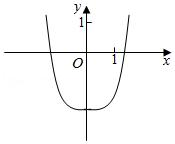
\includegraphics[width=.42\linewidth]{assets/asset-019-01.jpg}
\end{center}
\begin{choices}
  \item A
  \item B
  \item C
  \item D
\end{choices}
\begin{solution}
\textbf{答案：}D

\textbf{分析：}根据函数图象的特点，求函数的导数利用函数的单调性进行判断．

\textbf{详解：}函数过定点$(0,2)$，排除$A$、$B$．$f'(x)=-4x^3+2x=-2x(2x^2-1)$，令$f'(x)>0$得$x<-\frac{\sqrt{2}}{2}$或$0<x<\frac{\sqrt{2}}{2}$，此时函数递增；令$f'(x)<0$得$x>\frac{\sqrt{2}}{2}$或$-\frac{\sqrt{2}}{2}<x<0$，此时函数递减，排除$C$，故选$D$．
\end{solution}
\end{question}

\begin{question}[points=5]
\textbf{来源：}2018 年 全国III卷-理科，第 12 题\par
设$a=\log_{0.2}0.3$，$b=\log_2 0.3$，则（ ）
\begin{choices}
  \item $a+b<ab<0$
  \item $ab<a+b<0$
  \item $a+b<0<ab$
  \item $ab<0<a+b$
\end{choices}
\begin{solution}
\textbf{答案：}B

\textbf{分析：}直接利用对数的运算性质化简即可得答案．

\textbf{详解：}$a=\log_{0.2}0.3=\frac{\lg0.3}{\lg0.2}$，$b=\log_2 0.3=\frac{\lg0.3}{\lg2}$，$\because \lg0.3<0$，$\lg0.2<0$，$\lg2>0$，$\therefore a>0$，$b<0$，$ab<0$．又$\frac{1}{a}+\frac{1}{b}=\frac{\lg0.2}{\lg0.3}+\frac{\lg2}{\lg0.3}=\frac{\lg(0.2\times2)}{\lg0.3}=\frac{\lg0.4}{\lg0.3}$，$\because \lg0.4>\lg0.3$，$\therefore \frac{\lg0.4}{\lg0.3}<1$，$\frac{1}{a}+\frac{1}{b}<1$，即$\frac{a+b}{ab}<1$，$\because ab<0$，$\therefore a+b>ab$，故$ab<a+b<0$．
\end{solution}
\end{question}

\begin{question}[points=5]
\textbf{来源：}2018 年 全国III卷-文科，第 7 题\par
下列函数中，其图象与函数 $y=\ln x$ 的图象关于直线 $x=1$ 对称的是
\begin{choices}
  \item $y=\ln(1-x)$
  \item $y=\ln(2-x)$
  \item $y=\ln(1+x)$
  \item $y=\ln(2+x)$
\end{choices}
\begin{solution}
\textbf{答案：}B

\textbf{分析：}直接利用函数的图象的对称和平移变换求出结果．

\textbf{详解：}首先根据函数 $y=\ln x$ 的图象，则：函数 $y=\ln x$ 的图象与 $y=\ln(-x)$ 的图象关于 $y$ 轴对称．由于函数 $y=\ln x$ 的图象关于直线 $x=1$ 对称．则：把函数 $y=\ln(-x)$ 的图象向右平移 2 个单位即可得到：$y=\ln(2-x)$．即所求得解析式为：$y=\ln(2-x)$．故选：B．
\end{solution}
\end{question}

\begin{question}[points=5]
\textbf{来源：}2018 年 全国III卷-文科，第 9 题\par
函数 $y=-x^4+x^2+2$ 的图象大致为

\begin{center}
  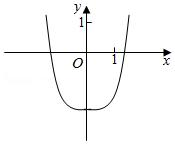
\includegraphics[width=.42\linewidth]{assets/asset-022-01.jpg}
\end{center}

\begin{center}
  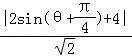
\includegraphics[width=.42\linewidth]{assets/asset-022-02.jpg}
\end{center}
\begin{choices}
  \item A
  \item B
  \item C
  \item D
\end{choices}
\begin{solution}
\textbf{答案：}D

\textbf{分析：}根据函数图象的特点，求函数的导数利用函数的单调性进行判断即可．

\textbf{详解：}函数过定点 $(0,2)$，排除 $A,B$．函数的导数 $f'(x)=-4x^3+2x=-2x(2x^2-1)$，由 $f'(x)>0$ 得 $2x(2x^2-1)<0$，得 $x<-\frac{\sqrt{2}}{2}$ 或 $0<x<\frac{\sqrt{2}}{2}$，此时函数单调递增；由 $f'(x)<0$ 得 $2x(2x^2-1)>0$，得 $x>\frac{\sqrt{2}}{2}$ 或 $-\frac{\sqrt{2}}{2}<x<0$，此时函数单调递减，排除 $C$．故选：D．
\end{solution}
\end{question}

\begin{question}[points=5]
\textbf{来源：}2018 年 全国III卷-文科，第 16 题\par
已知函数 $f(x)=\ln(\sqrt{1+x^2}-x)+1$，$f(a)=4$，则 $f(-a)=$
\fillin[{$-2$}]
\begin{solution}
\textbf{答案：}$-2$

\textbf{分析：}利用函数的奇偶性的性质以及函数值，转化求解即可．

\textbf{详解：}函数 $g(x)=\ln(\sqrt{1+x^2}-x)$ 满足 $g(-x)=\ln(\sqrt{1+x^2}+x)=\ln\frac{1}{\sqrt{1+x^2}-x}=-\ln(\sqrt{1+x^2}-x)=-g(x)$，所以 $g(x)$ 是奇函数．函数 $f(x)=\ln(\sqrt{1+x^2}-x)+1$，$f(a)=4$，可得 $f(a)=4=\ln(\sqrt{1+a^2}-a)+1$，可得 $\ln(\sqrt{1+a^2}-a)=3$，则 $f(-a)=-\ln(\sqrt{1+a^2}-a)+1=-3+1=-2$．故答案为：$-2$．
\end{solution}
\end{question}

\begin{question}[points=5]
\textbf{来源：}2018 年 全国II卷-理科，第 3 题\par
函数$f(x)=\frac{e^x-e^{-x}}{x^2}$的图象大致为（      ）
\begin{choices}
  \item 
  \item 
  \item 
  \item 
\end{choices}
\begin{solution}
\textbf{答案：}B

\textbf{分析：}判断函数的奇偶性，利用函数的定点的符号的特点分别进行判断即可．

\textbf{详解：}函数$f(-x)=\frac{e^{-x}-e^x}{x^2}=-\frac{e^x-e^{-x}}{x^2}=-f(x)$，则函数$f(x)$为奇函数，图象关于原点对称，排除A；当$x=1$时，$f(1)=e-e^{-1}>0$，排除D；当$x\to +\infty$时，$f(x)\to +\infty$，排除C，故选B．
\end{solution}
\end{question}

\begin{question}[points=5]
\textbf{来源：}2018 年 全国II卷-理科，第 11 题\par
已知$f(x)$是定义域为$(-\infty,+\infty)$的奇函数，满足$f(1-x)=f(1+x)$，若$f(1)=2$，则$f(1)+f(2)+f(3)+\cdots+f(50)=$（          ）
\begin{choices}
  \item $-50$
  \item $0$
  \item $2$
  \item $50$
\end{choices}
\begin{solution}
\textbf{答案：}C

\textbf{分析：}根据函数奇偶性和对称性的关系求出函数的周期是$4$，结合函数的周期性和奇偶性进行转化求解即可．

\textbf{详解：}$f(x)$是奇函数，且$f(1-x)=f(1+x)$，$\therefore f(1-x)=f(1+x)=-f(x-1)$，$f(0)=0$，则$f(x+2)=-f(x)$，则$f(x+4)=-f(x+2)=f(x)$，即函数$f(x)$是周期为$4$的周期函数，$f(1)=2$，$\therefore f(2)=f(0)=0$，$f(3)=f(1-2)=f(-1)=-f(1)=-2$，$f(4)=f(0)=0$，则$f(1)+f(2)+f(3)+f(4)=2+0-2+0=0$，则$f(1)+f(2)+f(3)+\cdots+f(50)=12[f(1)+f(2)+f(3)+f(4)]+f(49)+f(50)=f(1)+f(2)=2+0=2$，故选C．
\end{solution}
\end{question}

\begin{question}[points=5]
\textbf{来源：}2018 年 全国II卷-文科，第 3 题\par
函数 $f(x)=\frac{e^x-e^{-x}}{x^2}$ 的图象大致为（ ）

\begin{center}
  
\includegraphics[width=.42\linewidth]{assets/asset-026-01.jpg}
\end{center}
\begin{choices}
  \item 
  \item 
  \item 
  \item 
\end{choices}
\begin{solution}
\textbf{答案：}B

\textbf{分析：}判断函数的奇偶性，利用函数的定点的符号的特点分别进行判断即可。

\textbf{详解：}函数 $f(-x)=\frac{e^{-x}-e^{x}}{x^2}=-\frac{e^x-e^{-x}}{x^2}=-f(x)$，则函数 $f(x)$ 为奇函数，图象关于原点对称，排除 A，当 $x=1$ 时，$f(1)=e-\frac{1}{e}>0$，排除 D。当 $x\to+\infty$ 时，$f(x)\to+\infty$，排除 C，故选：B。
\end{solution}
\end{question}

\begin{question}[points=5]
\textbf{来源：}2018 年 全国II卷-文科，第 12 题\par
已知 $f(x)$ 是定义域为 $(-\infty,+\infty)$ 的奇函数，满足 $f(1-x)=f(1+x)$，若 $f(1)=2$，则 $f(1)+f(2)+f(3)+\cdots+f(50)=$（ ）
\begin{choices}
  \item $-50$
  \item $0$
  \item $2$
  \item $50$
\end{choices}
\begin{solution}
\textbf{答案：}$2$

\textbf{分析：}根据函数奇偶性和对称性的关系求出函数的周期是 4，结合函数的周期性和奇偶性进行转化求解即可。

\textbf{详解：}因为$f(x)$ 是奇函数，且 $f(1-x)=f(1+x)$，所以$f(1-x)=f(1+x)=-f(x-1)$，$f(0)=0$，则 $f(x+2)=-f(x)$，则 $f(x+4)=-f(x+2)=f(x)$，即函数 $f(x)$ 是周期为 4 的周期函数，因为$f(1)=2$，所以$f(2)=f(0)=0$，$f(3)=f(1-2)=f(-1)=-f(1)=-2$，$f(4)=f(0)=0$，则 $f(1)+f(2)+f(3)+f(4)=2+0-2+0=0$，则 $f(1)+f(2)+f(3)+\cdots+f(50)=12\times0+f(49)+f(50)=f(1)+f(2)=2+0=2$，故选：C。
\end{solution}
\end{question}

\begin{question}[points=5]
\textbf{来源：}2018 年 全国I卷-理科，第 9 题\par
已知函数$f(x)=\begin{cases} e^x, & x\leq0 \\ \ln x, & x>0 \end{cases}$，$g(x)=f(x)+x+a$。若$g(x)$存在2个零点，则$a$的取值范围是（    ）

\begin{center}
  
\includegraphics[width=.42\linewidth]{assets/asset-028-01.jpg}
\end{center}
\begin{choices}
  \item $[-1,0)$
  \item $[0,+\infty)$
  \item $[-1,+\infty)$
  \item $[1,+\infty)$
\end{choices}
\begin{solution}
\textbf{答案：}C

\textbf{分析：}由$g(x)=0$得$f(x)=-x-a$，分别作出两个函数的图象，根据图象交点个数与函数零点之间的关系进行转化求解即可。

\textbf{详解：}由$g(x)=0$得$f(x)=-x-a$，作出函数$f(x)$和$y=-x-a$的图象。当直线$y=-x-a$的截距$-a\leq1$，即$a\geq-1$时，两个函数的图象都有2个交点，即函数$g(x)$存在2个零点。故实数$a$的取值范围是$[-1,+\infty)$。故选C。
\end{solution}
\end{question}

\begin{question}[points=5]
\textbf{来源：}2018 年 全国I卷-文科，第 12 题\par
设函数 $f(x)=\begin{cases} 2^{-x}, & x\le 0 \\ 1, & x>0 \end{cases}$，则满足 $f(x+1)<f(2x)$ 的 $x$ 的取值范围是
\begin{choices}
  \item $(-\infty,-1]$
  \item $(0,+\infty)$
  \item $(-1,0)$
  \item $(-\infty,0)$
\end{choices}
\begin{solution}
\textbf{答案：}$(-\infty,0)$

\textbf{分析：}画出函数的图象，利用函数的单调性列出不等式转化求解即可。

\textbf{详解：}函数 $f(x)=\begin{cases} 2^{-x}, & x\le 0 \\ 1, & x>0 \end{cases}$ 的图象如图：满足 $f(x+1)<f(2x)$，可得 $2x<0<x+1$ 或 $2x<x+1\le 0$，解得 $x\in(-\infty,0)$。故选：$D$。
\end{solution}
\end{question}

\begin{question}[points=5]
\textbf{来源：}2018 年 全国I卷-文科，第 13 题\par
已知函数 $f(x)=\log_2(x^2+a)$，若 $f(3)=1$，则 $a=$
\fillin[{$-7$}]
\begin{solution}
\textbf{答案：}$-7$

\textbf{分析：}直接利用函数的解析式，求解函数值即可。

\textbf{详解：}函数 $f(x)=\log_2(x^2+a)$，若 $f(3)=1$，可得 $\log_2(9+a)=1$，可得 $a=-7$。故答案为：$-7$。
\end{solution}
\end{question}

\section*{2019 年}

\begin{question}[points=5]
\textbf{来源：}2019 年 全国III卷-理科，第 7 题\par
函数 $y = \dfrac{2x^3}{2^x + 2^{-x}}$ 在 $[-6,6]$ 的图象大致为

\begin{center}
  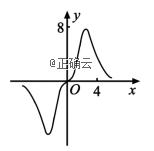
\includegraphics[width=.42\linewidth]{assets/asset-031-01.jpg}
\end{center}
\begin{choices}
  \item A
  \item B
  \item C
  \item D
\end{choices}
\begin{solution}
\textbf{答案：}B

\textbf{分析：}由分子、分母的奇偶性，易于确定函数为奇函数，由 $f(4)$ 的近似值即可得出结果。

\textbf{详解：}设 $y = f(x) = \dfrac{2x^3}{2^x + 2^{-x}}$，则 $f(-x) = \dfrac{2(-x)^3}{2^{-x} + 2^x} = -\dfrac{2x^3}{2^x + 2^{-x}} = -f(x)$，所以 $f(x)$ 是奇函数，图象关于原点对称，排除 C。又 $f(4) = \dfrac{2\times 4^3}{2^4 + 2^{-4}} > 0$，排除 D；$f(6) = \dfrac{2\times 6^3}{2^6 + 2^{-6}} \approx 7$，排除 A。故选 B。
\end{solution}
\end{question}

\begin{question}[points=5]
\textbf{来源：}2019 年 全国III卷-理科，第 11 题\par
设 $f(x)$ 是定义域为 $\mathbb{R}$ 的偶函数，且在 $(0,+\infty)$ 单调递减，则
\begin{choices}
  \item $f\left(\log_3\dfrac{1}{4}\right) > f\left(2^{-\frac{3}{2}}\right) > f\left(2^{-\frac{2}{3}}\right)$
  \item $f\left(\log_3\dfrac{1}{4}\right) > f\left(2^{-\frac{2}{3}}\right) > f\left(2^{-\frac{3}{2}}\right)$
  \item $f\left(2^{-\frac{3}{2}}\right) > f\left(2^{-\frac{2}{3}}\right) > f\left(\log_3\dfrac{1}{4}\right)$
  \item $f\left(2^{-\frac{2}{3}}\right) > f\left(2^{-\frac{3}{2}}\right) > f\left(\log_3\dfrac{1}{4}\right)$
\end{choices}
\begin{solution}
\textbf{答案：}C

\textbf{分析：}利用偶函数和单调性比较大小。

\textbf{详解：}因为 $f(x)$ 是偶函数，所以 $f\left(\log_3\dfrac{1}{4}\right) = f(\log_3 4)$。由于 $\log_3 4 > 1 = 2^0 > 2^{-\frac{2}{3}} > 2^{-\frac{3}{2}} > 0$，且 $f(x)$ 在 $(0,+\infty)$ 单调递减，所以 $f(\log_3 4) < f\left(2^{-\frac{2}{3}}\right) < f\left(2^{-\frac{3}{2}}\right)$，即 $f\left(2^{-\frac{3}{2}}\right) > f\left(2^{-\frac{2}{3}}\right) > f\left(\log_3\dfrac{1}{4}\right)$。故选 C。
\end{solution}
\end{question}

\begin{question}[points=5]
\textbf{来源：}2019 年 全国III卷-文科，第 12 题\par
设$f(x)$是定义域为R的偶函数，且在$(0,+\infty)$单调递减，则
\begin{choices}
  \item $f(\log_3\frac{1}{4})>f(2^{-\frac{3}{2}})>f(2^{-\frac{2}{3}})$
  \item $f(\log_3\frac{1}{4})>f(2^{-\frac{2}{3}})>f(2^{-\frac{3}{2}})$
  \item $f(2^{-\frac{3}{2}})>f(2^{-\frac{2}{3}})>f(\log_3\frac{1}{4})$
  \item $f(2^{-\frac{2}{3}})>f(2^{-\frac{3}{2}})>f(\log_3\frac{1}{4})$
\end{choices}
\begin{solution}
\textbf{答案：}C

\textbf{分析：}由已知函数为偶函数，把$f(\log_3\frac{1}{4}), f(2^{-\frac{3}{2}}), f(2^{-\frac{2}{3}})$转化为同一个单调区间上，再比较大小。

\textbf{详解：}$\because f(x)$是R的偶函数，$\therefore f(\log_3\frac{1}{4})=f(\log_3 4)$。$\log_3 4>1=2^0>2^{-\frac{1}{2}}$，又$f(x)$在$(0,+\infty)$单调递减，$\therefore f(\log_3 4)<f(2^{-\frac{2}{3}})<f(2^{-\frac{3}{2}})$，$\therefore f(2^{-\frac{3}{2}})>f(2^{-\frac{2}{3}})>f(\log_3\frac{1}{4})$，故选C。
\end{solution}
\end{question}

\begin{question}[points=5]
\textbf{来源：}2019 年 全国II卷-理科，第 4 题\par
2019 年 1 月 3 日嫦娥四号探测器成功实现人类历史上首次月球背面软着陆，我国航天事业取得又一重大成就，实现月球背面软着陆需要解决的一个关键技术问题是地面与探测器的通讯联系．为解决这个问题，发射了嫦娥四号中继星“鹊桥”，鹊桥沿着围绕地月拉格朗日 $L_2$ 点的轨道运行．$L_2$ 点是平衡点，位于地月连线的延长线上．设地球质量为 $M_1$，月球质量为 $M_2$，地月距离为 $R$，$L_2$ 点到月球的距离为 $r$，根据牛顿运动定律和万有引力定律，$r$ 满足方程：$\frac{M_1}{(R+r)^2}+\frac{M_2}{r^2}=(R+r)\frac{M_1}{R^3}$．设 $\alpha=\frac{r}{R}$，由于 $\alpha$ 的值很小，因此在近似计算中 $\frac{3\alpha^3+3\alpha^4+\alpha^5}{(1+\alpha)^2}\approx 3\alpha^3$，则 $r$ 的近似值为
\begin{choices}
  \item $\sqrt{\frac{M_2}{M_1}}R$
  \item $\sqrt{\frac{M_2}{2M_1}}R$
  \item $\sqrt[3]{\frac{3M_2}{M_1}}R$
  \item $\sqrt[3]{\frac{M_2}{3M_1}}R$
\end{choices}
\begin{solution}
\textbf{答案：}$D$

\textbf{分析：}本题在正确理解题意的基础上，将有关式子代入给定公式，建立 $\alpha$ 的方程，解方程、近似计算．

\textbf{详解：}由 $\alpha=\frac{r}{R}$，得 $r=\alpha R$．因为 $\frac{M_1}{(R+r)^2}+\frac{M_2}{r^2}=(R+r)\frac{M_1}{R^3}$，所以 $\frac{M_1}{R^2(1+\alpha)^2}+\frac{M_2}{\alpha^2 R^2}=(1+\alpha)\frac{M_1}{R^2}$，即 $\frac{M_2}{M_1}=\alpha^2[(1+\alpha)-\frac{1}{(1+\alpha)^2}]=\frac{\alpha^5+3\alpha^4+3\alpha^3}{(1+\alpha)^2}\approx 3\alpha^3$，解得 $\alpha=\sqrt[3]{\frac{M_2}{3M_1}}$，所以 $r=\alpha R=\sqrt[3]{\frac{M_2}{3M_1}}R$．故选 $D$．
\end{solution}
\end{question}

\begin{question}[points=5]
\textbf{来源：}2019 年 全国II卷-理科，第 12 题\par
设函数 $f(x)$ 的定义域为 $\mathbf{R}$，满足 $f(x+1)=2f(x)$，且当 $x\in(0,1]$ 时，$f(x)=x(x-1)$．若对任意 $x\in(-\infty,m]$，都有 $f(x)\geq -\frac{8}{9}$，则 $m$ 的取值范围是
\begin{choices}
  \item $(-\infty,\frac{9}{4}]$
  \item $(-\infty,\frac{7}{3}]$
  \item $(-\infty,\frac{5}{2}]$
  \item $(-\infty,\frac{8}{3}]$
\end{choices}
\begin{solution}
\textbf{答案：}$B$

\textbf{分析：}本题为选择压轴题，考查函数平移伸缩，恒成立问题，需准确求出函数每一段解析式，分析出临界点位置，精准运算得到解决．

\textbf{详解：}$\because x\in(0,1]$ 时，$f(x)=x(x-1)$，$f(x+1)=2f(x)$，$\therefore f(x)=2f(x-1)$，即 $f(x)$ 右移 1 个单位，图像变为原来的 2 倍．如图所示：当 $2<x\leq 3$ 时，$f(x)=4f(x-2)=4(x-2)(x-3)$，令 $4(x-2)(x-3)=-\frac{8}{9}$，整理得 $9x^2-45x+56=0$，$\therefore (3x-7)(3x-8)=0$，$\therefore x_1=\frac{7}{3},x_2=\frac{8}{3}$（舍），$\therefore x\in(-\infty,m]$ 时，$f(x)\geq -\frac{8}{9}$ 成立，即 $m\leq \frac{7}{3}$，$\therefore m\in(-\infty,\frac{7}{3}]$，故选 $B$．
\end{solution}
\end{question}

\begin{question}[points=5]
\textbf{来源：}2019 年 全国II卷-理科，第 14 题\par
已知 $f(x)$ 是奇函数，且当 $x<0$ 时，$f(x)=-e^{ax}$．若 $f(\ln 2)=8$，则 $a=$ .
\fillin[{$-3$}]
\begin{solution}
\textbf{答案：}$-3$

\textbf{分析：}本题主要考查函数奇偶性，对数的计算．渗透了数学运算、直观想象素养．使用转化思想得出答案．

\textbf{详解：}因为 $f(x)$ 是奇函数，且当 $x<0$ 时，$f(x)=-e^{ax}$．又因为 $\ln 2\in(0,1)$，$f(\ln 2)=8$，所以 $-e^{-a\ln 2}=-8$，两边取以 $e$ 为底的对数得 $-a\ln 2=3\ln 2$，所以 $-a=3$，即 $a=-3$．
\end{solution}
\end{question}

\begin{question}[points=5]
\textbf{来源：}2019 年 全国II卷-文科，第 6 题\par
设 $f(x)$ 为奇函数，且当 $x\geq 0$ 时，$f(x)=\mathrm{e}^x-1$，则当 $x<0$ 时，$f(x)=$
\begin{choices}
  \item $\mathrm{e}^{-x}-1$
  \item $\mathrm{e}^{-x}+1$
  \item $-\mathrm{e}^{-x}-1$
  \item $-\mathrm{e}^{-x}+1$
\end{choices}
\begin{solution}
\textbf{答案：}$D$

\textbf{分析：}先把 $x<0$，转化为 $-x>0$，代入可得 $f(-x)$，结合奇偶性可得 $f(x)$．

\textbf{详解：}$\because f(x)$ 是奇函数，当 $x<0$ 时，$-x>0$，$f(-x)=\mathrm{e}^{-x}-1=-f(x)$，得 $f(x)=-\mathrm{e}^{-x}+1$．故选 $D$．
\end{solution}
\end{question}

\begin{question}[points=5]
\textbf{来源：}2019 年 全国I卷-理科，第 3 题\par
已知 $a = \log_2 0.2$, $b = 2^{0.2}$, $c = 0.2^{0.3}$, 则
\begin{choices}
  \item $a < b < c$
  \item $a < c < b$
  \item $c < a < b$
  \item $b < c < a$
\end{choices}
\begin{solution}
\textbf{答案：}$B$

\textbf{分析：}运用中间量 $0$ 比较 $a$, $c$，运用中间量 $1$ 比较 $b$, $c$．

\textbf{详解：}$a = \log_2 0.2 < \log_2 1 = 0$, $b = 2^{0.2} > 2^0 = 1$, $0 < 0.2^{0.3} < 0.2^0 = 1$, 则 $0 < c < 1$, $a < c < b$．故选 $B$．
\end{solution}
\end{question}

\begin{question}[points=5]
\textbf{来源：}2019 年 全国I卷-理科，第 4 题\par
古希腊时期，人们认为最美人体的头顶至肚脐的长度与肚脐至足底的长度之比是 $\frac{\sqrt{5} - 1}{2}$ ( $\frac{\sqrt{5} - 1}{2} \approx 0.618$ ，称为黄金分割比例)，著名的“断臂维纳斯”便是如此．此外，最美人体的头顶至咽喉的长度与咽喉至肚脐的长度之比也是 $\frac{\sqrt{5} - 1}{2}$ ．若某人满足上述两个黄金分割比例，且腿长为 $105$ cm，头顶至脖子下端的长度为 $26$ cm，则其身高可能是
\begin{choices}
  \item $165$ cm
  \item $175$ cm
  \item $185$ cm
  \item $190$ cm
\end{choices}
\begin{solution}
\textbf{答案：}$B$

\textbf{分析：}理解黄金分割比例的含义，应用比例式列方程求解．

\textbf{详解：}设人体脖子下端至腿根的长为 $x$ cm，肚脐至腿根的长为 $y$ cm，则 $\frac{26}{x} = \frac{26 + x}{y + 105} = \frac{\sqrt{5} - 1}{2}$，得 $x \approx 42.07$ cm, $y \approx 5.15$ cm．又其腿长为 $105$ cm，头顶至脖子下端的长度为 $26$ cm，所以其身高约为 $42.07 + 5.15 + 105 + 26 = 178.22$，接近 $175$ cm．故选 $B$．
\end{solution}
\end{question}

\begin{question}[points=5]
\textbf{来源：}2019 年 全国I卷-理科，第 5 题\par
函数 $f(x) = \frac{\sin x + x}{\cos x + x^2}$ 在 $[-\pi, \pi]$ 的图像大致为

\begin{center}
  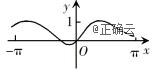
\includegraphics[width=.42\linewidth]{assets/asset-040-01.jpg}
\end{center}
\begin{choices}
  \item A． (图片)
  \item B． (图片)
  \item C． (图片)
  \item D． (图片)
\end{choices}
\begin{solution}
\textbf{答案：}$D$

\textbf{分析：}先判断函数的奇偶性，得 $f(x)$ 是奇函数，排除 $A$，再注意到选项的区别，利用特殊值得正确答案．

\textbf{详解：}由 $f(-x) = \frac{\sin(-x) + (-x)}{\cos(-x) + (-x)^2} = \frac{-\sin x - x}{\cos x + x^2} = -f(x)$，得 $f(x)$ 是奇函数，其图象关于原点对称．又 $f\left(\frac{\pi}{2}\right) = \frac{1 + \frac{\pi}{2}}{\left(\frac{\pi}{2}\right)^2} = \frac{4 + 2\pi}{\pi^2} > 1$, $f(\pi) = \frac{\pi}{-1 + \pi^2} > 0$．故选 $D$．
\end{solution}
\end{question}

\begin{question}[points=5]
\textbf{来源：}2019 年 全国I卷-文科，第 3 题\par
已知 $a = \log_2 0.2$，$b = 2^{0.2}$，$c = 0.2^{0.3}$，则
\begin{choices}
  \item $a < b < c$
  \item $a < c < b$
  \item $c < a < b$
  \item $b < c < a$
\end{choices}
\begin{solution}
\textbf{答案：}B

\textbf{分析：}运用中间量 0 比较 $a$，$c$，运用中间量 1 比较 $b$，$c$。

\textbf{详解：}$a = \log_2 0.2 < \log_2 1 = 0$，$b = 2^{0.2} > 2^0 = 1$，$0 < 0.2^{0.3} < 0.2^0 = 1$，则 $0 < c < 1$，$a < c < b$。故选 B。
\end{solution}
\end{question}

\begin{question}[points=5]
\textbf{来源：}2019 年 全国I卷-文科，第 4 题\par
古希腊时期，人们认为最美人体的头顶至肚脐的长度与肚脐至足底的长度之比是 $\frac{\sqrt{5}-1}{2}$（$\frac{\sqrt{5}-1}{2} \approx 0.618$，称为黄金分割比例)，著名的“断臂维纳斯”便是如此．此外，最美人体的头顶至咽喉的长度与咽喉至肚脐的长度之比也是 $\frac{\sqrt{5}-1}{2}$．若某人满足上述两个黄金分割比例，且腿长为 105cm，头顶至脖子下端的长度为 26 cm，则其身高可能是
\begin{choices}
  \item 165 cm
  \item 175 cm
  \item 185 cm
  \item 190 cm
\end{choices}
\begin{solution}
\textbf{答案：}B

\textbf{分析：}理解黄金分割比例的含义，应用比例式列方程求解。

\textbf{详解：}设人体脖子下端至腿根的长为 $x$ cm，肚脐至腿根的长为 $y$ cm，则 $\frac{26}{x} = \frac{26+x}{y+105} = \frac{\sqrt{5}-1}{2}$，得 $x \approx 42.07$ cm，$y \approx 5.15$ cm．又其腿长为 105cm，头顶至脖子下端的长度为 26cm，所以其身高约为 42.07+5.15+105+26=178.22，接近 175cm．故选 B。
\end{solution}
\end{question}

\begin{question}[points=5]
\textbf{来源：}2019 年 全国I卷-文科，第 5 题\par
函数 $f(x)=\frac{\sin x + x}{\cos x + x^2}$ 在 $[-\pi,\pi]$ 的图像大致为
\begin{choices}
  \item A
  \item B
  \item C
  \item D
\end{choices}
\begin{solution}
\textbf{答案：}D

\textbf{分析：}先判断函数的奇偶性，得 $f(x)$ 是奇函数，排除 A，再注意到选项的区别，利用特殊值得正确答案。

\textbf{详解：}由 $f(-x)=\frac{\sin(-x)+(-x)}{\cos(-x)+(-x)^2} = \frac{-\sin x - x}{\cos x + x^2} = -f(x)$，得 $f(x)$ 是奇函数，其图象关于原点对称．又 $f(\frac{\pi}{2}) = \frac{1+\frac{\pi}{2}}{(\frac{\pi}{2})^2} = \frac{4+2\pi}{\pi^2} > 1$，$f(\pi) = \frac{\pi}{-1+\pi^2} > 0$。故选 D。
\end{solution}
\end{question}

\section*{2020 年}

\begin{question}[points=5]
\textbf{来源：}2020 年 全国III卷-理科，第 4 题\par
Logistic 模型是常用数学模型之一，可应用于流行病学领域。有学者根据公布数据建立了某地区新冠肺炎累计确诊病例数 $I(t)$ ($t$ 的单位：天)的 Logistic 模型：$I(t)=\dfrac{K}{1+e^{-0.23(t-53)}}$，其中 $K$ 为最大确诊病例数。当 $I(t^*)=0.95K$ 时，标志着已初步遏制疫情，则 $t^*$ 约为 ($\ln 19\approx 3$)
\begin{choices}
  \item $60$
  \item $63$
  \item $66$
  \item $69$
\end{choices}
\begin{solution}
\textbf{答案：}$C$

\textbf{分析：}将 $t=t^*$ 代入函数 $I(t)=\dfrac{K}{1+e^{-0.23(t-53)}}$ 结合 $I(t^*)=0.95K$ 求得 $t^*$ 即可得解。

\textbf{详解：}因为 $I(t)=\dfrac{K}{1+e^{-0.23(t-53)}}$，所以 $I(t^*)=\dfrac{K}{1+e^{-0.23(t^*-53)}}=0.95K$，则 $e^{0.23(t^*-53)}=19$，所以 $0.23(t^*-53)=\ln 19\approx3$，解得 $t^*\approx\dfrac{3}{0.23}+53\approx66$。故选 $C$。
\end{solution}
\end{question}

\begin{question}[points=5]
\textbf{来源：}2020 年 全国III卷-理科，第 12 题\par
已知 $5^5<8^4$，$13^4<8^5$。设 $a=\log_5 3$，$b=\log_8 5$，$c=\log_{13}8$，则
\begin{choices}
  \item $a<b<c$
  \item $b<a<c$
  \item $b<c<a$
  \item $c<a<b$
\end{choices}
\begin{solution}
\textbf{答案：}$A$

\textbf{分析：}比较 $a,b,c$ 的大小，可先判断范围，再通过作商法、指数式与对数式互化进行比较。

\textbf{详解：}由题意知 $a,b,c\in(0,1)$。$\dfrac{a}{b}=\dfrac{\log_53}{\log_85}=\dfrac{\lg3}{\lg5}\cdot\dfrac{\lg8}{\lg5}<\dfrac{1}{2}\left(\dfrac{\lg3+\lg8}{\lg5}\right)^2=\left(\dfrac{\lg24}{\lg25}\right)^2<1$，所以 $a<b$。由 $b=\log_85$ 得 $8^b=5$，由 $5^5<8^4$ 得 $8^{5b}<8^4$，所以 $5b<4$，$b<\dfrac45$。由 $c=\log_{13}8$ 得 $13^c=8$，由 $13^4<8^5$ 得 $13^4<13^{5c}$，所以 $4<5c$，$c>\dfrac45$。综上 $a<b<c$。故选 $A$。
\end{solution}
\end{question}

\begin{question}[points=5]
\textbf{来源：}2020 年 全国III卷-文科，第 4 题\par
Logistic 模型是常用数学模型之一，可应用于流行病学领域. 有学者根据公布数据建立了某地区新冠肺炎累计确诊病例数 $I(t)$ ($t$ 的单位：天)的 Logistic 模型：$I(t)=\frac{K}{1+e^{-0.23(t-53)}}$，其中 $K$ 为最大确诊病例数. 当 $I(t^*)=0.95K$ 时，标志着已初步遏制疫情，则 $t^*$ 约为 ( $\ln19\approx3$ )
\begin{choices}
  \item $60$
  \item $63$
  \item $66$
  \item $69$
\end{choices}
\begin{solution}
\textbf{答案：}C

\textbf{分析：}将 $t=t^*$ 代入函数 $I(t)=\frac{K}{1+e^{-0.23(t-53)}}$ 结合 $I(t^*)=0.95K$ 求得 $t^*$ 即可得解.

\textbf{详解：}因为 $I(t)=\frac{K}{1+e^{-0.23(t-53)}}$，所以 $I(t^*)=\frac{K}{1+e^{-0.23(t^*-53)}}=0.95K$，则 $e^{0.23(t^*-53)}=19$，所以 $0.23(t^*-53)=\ln19\approx3$，解得 $t^*\approx\frac{3}{0.23}+53\approx66$. 故选：C.
\end{solution}
\end{question}

\begin{question}[points=5]
\textbf{来源：}2020 年 全国III卷-文科，第 10 题\par
设 $a=\log_32$，$b=\log_53$，$c=\frac{2}{3}$，则
\begin{choices}
  \item $a<c<b$
  \item $a<b<c$
  \item $b<c<a$
  \item $c<a<b$
\end{choices}
\begin{solution}
\textbf{答案：}A

\textbf{分析：}分别将 $a,b$ 改写为 $a=\frac{1}{3}\log_32^3$，$b=\frac{1}{3}\log_53^3$，再利用单调性比较即可.

\textbf{详解：}因为 $a=\frac{1}{3}\log_32^3<\frac{1}{3}\log_39=\frac{2}{3}=c$，$b=\frac{1}{3}\log_53^3>\frac{1}{3}\log_525=\frac{2}{3}=c$，所以 $a<c<b$. 故选：A.
\end{solution}
\end{question}

\begin{question}[points=5]
\textbf{来源：}2020 年 全国II卷-理科，第 9 题\par
设函数$f(x)=\ln|2x+1|-\ln|2x-1|$，则$f(x)$（ ）
\begin{choices}
  \item 是偶函数，且在$(\frac12,+\infty)$单调递增
  \item 是奇函数，且在$(-\frac12,\frac12)$单调递减
  \item 是偶函数，且在$(-\infty,-\frac12)$单调递增
  \item 是奇函数，且在$(-\infty,-\frac12)$单调递减
\end{choices}
\begin{solution}
\textbf{答案：}是奇函数，且在$(-\infty,-\frac12)$单调递减

\textbf{分析：}根据奇偶性的定义可判断出$f(x)$为奇函数，排除AC；当$x\in(-\frac12,\frac12)$时，利用函数单调性的性质可判断出$f(x)$单调递增，排除B；当$x\in(-\infty,-\frac12)$时，利用复合函数单调性可判断出$f(x)$单调递减，从而得到结果.

\textbf{详解：}由$f(x)=\ln|2x+1|-\ln|2x-1|$得$f(x)$定义域为$\{x|x\neq\pm\frac12\}$，关于坐标原点对称，又$f(-x)=\ln|1-2x|-\ln|-2x-1|=\ln|2x-1|-\ln|2x+1|=-f(x)$，$\therefore f(x)$为定义域上的奇函数，排除AC；当$x\in(-\frac12,\frac12)$时，$f(x)=\ln(2x+1)-\ln(1-2x)$，$\because y=\ln(2x+1)$在$(-\frac12,\frac12)$上单调递增，$y=\ln(1-2x)$在$(-\frac12,\frac12)$上单调递减，$\therefore f(x)$在$(-\frac12,\frac12)$上单调递增，排除B；当$x\in(-\infty,-\frac12)$时，$f(x)=\ln(-2x-1)-\ln(1-2x)=\ln\dfrac{2x+1}{2x-1}=\ln\left(1+\dfrac{2}{2x-1}\right)$，$\because \mu=1+\dfrac{2}{2x-1}$在$(-\infty,-\frac12)$上单调递减，$f(\mu)=\ln\mu$在定义域内单调递增，根据复合函数单调性可知：$f(x)$在$(-\infty,-\frac12)$上单调递减，D正确.
\end{solution}
\end{question}

\begin{question}[points=5]
\textbf{来源：}2020 年 全国II卷-理科，第 11 题\par
若$2^x-2^y<3^{-x}-3^{-y}$，则（ ）
\begin{choices}
  \item $\ln(y-x+1)>0$
  \item $\ln(y-x+1)<0$
  \item $\ln|x-y|>0$
  \item $\ln|x-y|<0$
\end{choices}
\begin{solution}
\textbf{答案：}$\ln(y-x+1)>0$

\textbf{分析：}将不等式变为$2^x-3^{-x}<2^y-3^{-y}$，根据$f(t)=2^t-3^{-t}$的单调性知$x<y$，以此去判断各个选项中真数与1的大小关系，进而得到结果.

\textbf{详解：}由$2^x-2^y<3^{-x}-3^{-y}$得：$2^x-3^{-x}<2^y-3^{-y}$，令$f(t)=2^t-3^{-t}$，$\because y=2^x$为R上的增函数，$y=3^{-x}$为R上的减函数，$\therefore f(t)$为R上的增函数，$\therefore x<y$，$\because y-x>0$，$\therefore y-x+1>1$，$\therefore\ln(y-x+1)>0$，则A正确，B错误；$\because|x-y|$与1的大小不确定，故CD无法确定.
\end{solution}
\end{question}

\begin{question}[points=5]
\textbf{来源：}2020 年 全国II卷-文科，第 7 题\par
执行右面的程序框图，若输入的 $k=0$，$a=0$，则输出的 $k$ 为（ ）

\begin{center}
  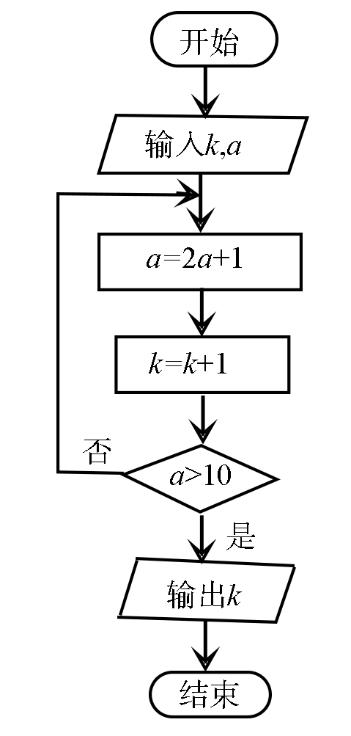
\includegraphics[width=.42\linewidth]{assets/asset-050-01.jpg}
\end{center}
\begin{choices}
  \item $2$
  \item $3$
  \item $4$
  \item $5$
\end{choices}
\begin{solution}
\textbf{答案：}C

\textbf{分析：}由已知中的程序框图可知：该程序的功能是利用循环结构计算并输出 $k$ 的值，模拟程序的运行过程，分析循环中各变量值的变化情况，即可求得答案。

\textbf{详解：}模拟程序的运行过程：
$k=0, a=0$
第1次循环，$a=2\times0+1=1$，$k=0+1=1$，$1>10$ 为否；
第2次循环，$a=2\times1+1=3$，$k=1+1=2$，$3>10$ 为否；
第3次循环，$a=2\times3+1=7$，$k=2+1=3$，$7>10$ 为否；
第4次循环，$a=2\times7+1=15$，$k=3+1=4$，$15>10$ 为是；
退出循环，输出 $k=4$。
故选：C。
\end{solution}
\end{question}

\begin{question}[points=5]
\textbf{来源：}2020 年 全国II卷-文科，第 10 题\par
设函数 $f(x)=x^3-\frac{1}{x^3}$，则 $f(x)$（ ）
\begin{choices}
  \item 是奇函数，且在 $(0,+\infty)$ 单调递增
  \item 是奇函数，且在 $(0,+\infty)$ 单调递减
  \item 是偶函数，且在 $(0,+\infty)$ 单调递增
  \item 是偶函数，且在 $(0,+\infty)$ 单调递减
\end{choices}
\begin{solution}
\textbf{答案：}A

\textbf{分析：}根据函数的解析式可知函数的定义域为 $\{x|x\neq0\}$，利用定义可得出函数 $f(x)$ 为奇函数，再根据函数的单调性法则，即可解出。

\textbf{详解：}因为函数 $f(x)=x^3-\frac{1}{x^3}$ 定义域为 $\{x|x\neq0\}$，关于原点对称，且 $f(-x) = -f(x)$，所以函数 $f(x)$ 为奇函数。
又因为 $y=x^3$ 在 $(0,+\infty)$ 上单调递增，$y=\frac{1}{x^3}=x^{-3}$ 在 $(0,+\infty)$ 上单调递减，所以 $f(x)=x^3-\frac{1}{x^3}$ 在 $(0,+\infty)$ 上单调递增。
故选：A。
\end{solution}
\end{question}

\begin{question}[points=5]
\textbf{来源：}2020 年 全国II卷-文科，第 12 题\par
若 $2^x-2^y < 3^{-x}-3^{-y}$，则（ ）
\begin{choices}
  \item $\ln(y-x+1)>0$
  \item $\ln(y-x+1)<0$
  \item $\ln|x-y|>0$
  \item $\ln|x-y|<0$
\end{choices}
\begin{solution}
\textbf{答案：}A

\textbf{分析：}将不等式变为 $2^x-3^{-x}<2^y-3^{-y}$，根据 $f(t)=2^t-3^{-t}$ 的单调性知 $x<y$，以此去判断各个选项中真数与1的大小关系，进而得到结果。

\textbf{详解：}由 $2^x-2^y < 3^{-x}-3^{-y}$ 得：$2^x-3^{-x} < 2^y-3^{-y}$。
令 $f(t)=2^t-3^{-t}$，$\because y=2^x$ 为 $\mathbb{R}$ 上的增函数，$y=3^{-x}$ 为 $\mathbb{R}$ 上的减函数，$\therefore f(t)$ 为 $\mathbb{R}$ 上的增函数。
$\therefore x<y$。
$\because y-x>0$，$\therefore y-x+1>1$，$\therefore \ln(y-x+1)>0$，则A正确，B错误。
$\because |x-y|$ 与1的大小不确定，故CD无法确定。
故选：A。
\end{solution}
\end{question}

\begin{question}[points=5]
\textbf{来源：}2020 年 全国I卷-理科，第 12 题\par
若$2^a+\log_2 a=4^b+2\log_4 b$，则
\begin{choices}
  \item $a>2b$
  \item $a<2b$
  \item $a>b^2$
  \item $a<b^2$
\end{choices}
\begin{solution}
\textbf{答案：}B

\textbf{详解：}设$f(x)=2^x+\log_2 x$，则$f(x)$为增函数。已知$2^a+\log_2 a=4^b+2\log_4 b=2^{2b}+\log_2 b$。计算$f(a)-f(2b)=2^a+\log_2 a-(2^{2b}+\log_2 2b)=2^{2b}+\log_2 b-(2^{2b}+\log_2 2b)=\log_2\frac{1}{2}=-1<0$，所以$f(a)<f(2b)$，故$a<2b$。
\end{solution}
\end{question}

\begin{question}[points=5]
\textbf{来源：}2020 年 全国I卷-文科，第 8 题\par
设 $a\log_3 4 = 2$, 则 $4^{-a} =$
\begin{choices}
  \item $\frac{1}{16}$
  \item $\frac{1}{9}$
  \item $\frac{1}{8}$
  \item $\frac{1}{6}$
\end{choices}
\begin{solution}
\textbf{答案：}$\frac{1}{9}$

\textbf{分析：}首先根据题中所给的式子，结合对数的运算法则，得到 $\log_3 4^a = 2$, 即 $4^a = 9$, 进而求得 $4^{-a} = \frac{1}{9}$.

\textbf{详解：}由 $a\log_3 4 = 2$ 可得 $\log_3 4^a = 2$, 所以 $4^a = 9$, 所以 $4^{-a} = \frac{1}{9}$.
\end{solution}
\end{question}

\section*{2021 年}

\begin{question}[points=5]
\textbf{来源：}2021 年 北京卷，第 15 题\par
已知函数 $f(x)=|\lg x|-kx-2$, 给出下列四个结论：

①若 $k=0$, 则 $f(x)$ 有两个零点；

② $\exists k<0$, 使得 $f(x)$ 有一个零点；

③ $\exists k<0$, 使得 $f(x)$ 有三个零点；

④ $\exists k>0$, 使得 $f(x)$ 有三个零点.

以上正确结论的序号是.
\fillin[{$①②④$}]
\begin{solution}
\textbf{答案：}$①②④$

\textbf{分析：}由 $f(x)=0$ 可得出 $|\lg x|=kx+2$, 考查直线 $y=kx+2$ 与曲线 $g(x)=|\lg x|$ 的左、右支分别相切的情形, 利用方程思想以及数形结合可判断各选项的正误.

\textbf{详解：}对于①, 当 $k=0$ 时, 由 $f(x)=|\lg x|-2=0$, 可得 $x=\frac{1}{100}$ 或 $x=100$, ①正确；
对于②, 考查直线 $y=kx+2$ 与曲线 $y=-\lg x(0<x<1)$ 相切于点 $P(t,-\lg t)$, 对函数 $y=-\lg x$ 求导得 $y'=-\frac{1}{x\ln 10}$, 由题意可得 $\begin{cases} kt+2=-\lg t \\ k=-\frac{1}{t\ln 10} \end{cases}$, 解得 $\begin{cases} t=\frac{e}{100} \\ k=-\frac{100}{e}\lg e<0 \end{cases}$, 所以存在 $k=-\frac{100}{e}\lg e<0$, 使得 $f(x)$ 只有一个零点, ②正确；
对于③, 当直线 $y=kx+2$ 过点 $(1,0)$ 时, $k+2=0$, 解得 $k=-2$, 所以当 $-\frac{100}{e}\lg e<k<-2$ 时, 直线 $y=kx+2$ 与曲线 $y=-\lg x(0<x<1)$ 有两个交点, 若函数 $f(x)$ 有三个零点, 则直线 $y=kx+2$ 与曲线 $y=-\lg x(0<x<1)$ 有两个交点, 直线 $y=kx+2$ 与曲线 $y=\lg x(x>1)$ 有一个交点, 所以 $\begin{cases} -\frac{100}{e}\lg e<k<-2 \\ k+2>0 \end{cases}$, 此不等式无解, 因此不存在 $k<0$, 使得函数 $f(x)$ 有三个零点, ③错误；
对于④, 考查直线 $y=kx+2$ 与曲线 $y=\lg x(x>1)$ 相切于点 $P(t,\lg t)$, 对函数 $y=\lg x$ 求导得 $y'=\frac{1}{x\ln 10}$, 由题意可得 $\begin{cases} kt+2=\lg t \\ k=\frac{1}{t\ln 10} \end{cases}$, 解得 $\begin{cases} t=100e \\ k=\frac{\lg e}{100e} \end{cases}$, 所以当 $0<k<\frac{\lg e}{100e}$ 时, 函数 $f(x)$ 有三个零点, ④正确.
\end{solution}
\end{question}

\begin{question}[points=5]
\textbf{来源：}2021 年 全国甲卷-理科，第 4 题\par
青少年视力是社会普遍关注的问题，视力情况可借助视力表测量．通常用五分记录法和小数记录法记录视力数据，五分记录法的数据 $L$ 和小数记录表的数据 $V$ 满足 $L = 5 + \lg V$．已知某同学视力的五分记录法的数据为 $4.9$，则其视力的小数记录法的数据为（ ）($\sqrt[10]{10} \approx 1.259$)
\begin{choices}
  \item $1.5$
  \item $1.2$
  \item $0.8$
  \item $0.6$
\end{choices}
\begin{solution}
\textbf{答案：}C

\textbf{分析：}根据 $L,V$ 关系，当 $L=4.9$ 时，求出 $\lg V$，再用指数表示 $V$，即可求解．

\textbf{详解：}由 $L=5+\lg V$，当 $L=4.9$ 时，$\lg V = -0.1$，则 $V = 10^{-0.1} = 10^{-\frac{1}{10}} = \frac{1}{\sqrt[10]{10}} \approx \frac{1}{1.259} \approx 0.8$．
\end{solution}
\end{question}

\begin{question}[points=5]
\textbf{来源：}2021 年 全国甲卷-理科，第 12 题\par
设函数 $f(x)$ 的定义域为 $\mathbb{R}$，$f(x+1)$ 为奇函数，$f(x+2)$ 为偶函数，当 $x \in [1,2]$ 时，$f(x) = ax^2 + b$．若 $f(0) + f(3) = 6$，则 $f\left(\frac{9}{2}\right) =$ ( )
\begin{choices}
  \item $-\frac{9}{4}$
  \item $-\frac{3}{2}$
  \item $\frac{7}{4}$
  \item $\frac{5}{2}$
\end{choices}
\begin{solution}
\textbf{答案：}D

\textbf{分析：}通过 $f(x+1)$ 是奇函数和 $f(x+2)$ 是偶函数条件，可以确定出函数解析式 $f(x) = -2x^2 + 2$，进而利用定义或周期性结论，即可得到答案．

\textbf{详解：}由 $f(x+1)$ 为奇函数得 $f(-x+1) = -f(x+1)$，由 $f(x+2)$ 为偶函数得 $f(x+2) = f(-x+2)$．令 $x=1$ 得 $f(0) = -f(2) = -(4a+b)$，$f(3) = f(1) = a+b$，代入 $f(0)+f(3)=6$ 得 $-(4a+b)+a+b=6$，解得 $a=-2$．令 $x=0$ 得 $f(1)=-f(1)$，故 $f(1)=0$，所以 $b=2$，则 $f(x) = -2x^2+2$．由对称性可得周期 $T=4$，故 $f\left(\frac{9}{2}\right) = f\left(\frac{1}{2}\right) = -f\left(\frac{3}{2}\right)$，而 $f\left(\frac{3}{2}\right) = -2\cdot\frac{9}{4}+2 = -\frac{5}{2}$，所以 $f\left(\frac{9}{2}\right) = \frac{5}{2}$．
\end{solution}
\end{question}

\begin{question}[points=5]
\textbf{来源：}2021 年 全国甲卷-文科，第 4 题\par
下列函数中是增函数的为（ ）
\begin{choices}
  \item $f(x) = -x$
  \item $f(x) = \left(\frac{2}{3}\right)^x$
  \item $f(x) = x^2$
  \item $f(x) = \sqrt[3]{x}$
\end{choices}
\begin{solution}
\textbf{答案：}D

\textbf{分析：}根据基本初等函数的性质逐项判断后可得正确的选项.

\textbf{详解：}对于A, $f(x)=-x$ 为 $\mathbb{R}$ 上的减函数，不合题意，舍.
对于B, $f(x)=\left(\frac{2}{3}\right)^x$ 为 $\mathbb{R}$ 上的减函数，不合题意，舍.
对于C, $f(x)=x^2$ 在 $(-\infty,0)$ 为减函数，不合题意，舍.
对于D, $f(x)=\sqrt[3]{x}$ 为 $\mathbb{R}$ 上的增函数，符合题意.
\end{solution}
\end{question}

\begin{question}[points=5]
\textbf{来源：}2021 年 全国甲卷-文科，第 6 题\par
青少年视力是社会普遍关注的问题，视力情况可借助视力表测量．通常用五分记录法和小数记录法记录视力数据，五分记录法的数据 $L$ 和小数记录表的数据 $V$ 的满足 $L = 5 + \lg V$．已知某同学视力的五分记录法的数据为4.9，则其视力的小数记录法的数据为（ ）（$\sqrt[10]{10} \approx 1.259$）
\begin{choices}
  \item 1.5
  \item 1.2
  \item 0.8
  \item 0.6
\end{choices}
\begin{solution}
\textbf{答案：}C

\textbf{分析：}根据 $L,V$ 关系，当 $L=4.9$ 时，求出 $\lg V$, 再用指数表示 $V$, 即可求解.

\textbf{详解：}由 $L=5+\lg V$, 当 $L=4.9$ 时, $\lg V = -0.1$, 则 $V = 10^{-0.1} = 10^{-\frac{1}{10}} = \frac{1}{\sqrt[10]{10}} \approx \frac{1}{1.259} \approx 0.8$.
\end{solution}
\end{question}

\begin{question}[points=5]
\textbf{来源：}2021 年 全国甲卷-文科，第 12 题\par
设 $f(x)$ 是定义域为 $\mathbf{R}$ 的奇函数，且 $f(1+x)=f(-x)$. 若 $f\left(-\frac{1}{3}\right) = \frac{1}{3}$, 则 $f\left(\frac{5}{3}\right) =$ ( )
\begin{choices}
  \item $-\frac{5}{3}$
  \item $-\frac{1}{3}$
  \item $\frac{1}{3}$
  \item $\frac{5}{3}$
\end{choices}
\begin{solution}
\textbf{答案：}C

\textbf{分析：}由题意利用函数的奇偶性和函数的递推关系即可求得 $f\left(\frac{5}{3}\right)$ 的值.

\textbf{详解：}$f\left(\frac{5}{3}\right) = f\left(1+\frac{2}{3}\right) = f\left(-\frac{2}{3}\right) = -f\left(\frac{2}{3}\right)$. 而 $f\left(\frac{2}{3}\right) = f\left(1-\frac{1}{3}\right) = f\left(\frac{1}{3}\right) = -f\left(-\frac{1}{3}\right) = -\frac{1}{3}$, 故 $f\left(\frac{5}{3}\right) = \frac{1}{3}$.
\end{solution}
\end{question}

\begin{question}[points=5]
\textbf{来源：}2021 年 全国乙卷-理科，第 4 题\par
设函数$f(x)=\frac{1-x}{1+x}$，则下列函数中为奇函数的是（  ）
\begin{choices}
  \item $f(x-1)-1$
  \item $f(x-1)+1$
  \item $f(x+1)-1$
  \item $f(x+1)+1$
\end{choices}
\begin{solution}
\textbf{答案：}$f(x-1)+1$

\textbf{详解：}$f(x)=\frac{1-x}{1+x}=-1+\frac{2}{1+x}$，$f(x)$向右平移一个单位，向上平移一个单位得到$g(x)=\frac{2}{x}$，为奇函数。故选B。
\end{solution}
\end{question}

\begin{question}[points=5]
\textbf{来源：}2021 年 全国乙卷-理科，第 12 题\par
设$a=2\ln1.01$，$b=\ln1.02$，$c=\sqrt{1.04}-1$，则（  ）
\begin{choices}
  \item $a<b<c$
  \item $b<c<a$
  \item $b<a<c$
  \item $c<a<b$
\end{choices}
\begin{solution}
\textbf{答案：}$b<c<a$

\textbf{详解：}设$f(x)=\ln(1+x)-\sqrt{1+2x}+1$，则$b-c=f(0.02)$，易得$f'(x)=\frac{1}{1+x}-\frac{1}{\sqrt{1+2x}}=\frac{\sqrt{1+2x}-(1+x)}{(1+x)\sqrt{1+2x}}$。当$x\geq0$时，$1+x=\sqrt{(1+x)^2}\geq\sqrt{1+2x}$，故$f'(x)\leq0$。所以$f(x)$在$[0,+\infty)$上单调递减，所以$f(0.02)<f(0)=0$，故$b<c$。再设$g(x)=2\ln(1+x)-\sqrt{1+4x}+1$，则$a-c=g(0.01)$，易得$g'(x)=\frac{2}{1+x}-\frac{2}{\sqrt{1+4x}}=2\cdot\frac{\sqrt{1+4x}-(1+x)}{(1+x)\sqrt{1+4x}}$。当$0\leq x<2$时，$\sqrt{1+4x}\geq 1+2x+x^2=1+x$，所以$g'(x)\geq0$。故$g(x)$在$[0,2)$上单调递增，所以$g(0.01)>g(0)=0$，故$a>c$。综上，$a>c>b$。故选B。
\end{solution}
\end{question}

\begin{question}[points=5]
\textbf{来源：}2021 年 全国乙卷-文科，第 9 题\par
设函数 $f(x) = \frac{1-x}{1+x}$ ，则下列函数中为奇函数的是（ ）
\begin{choices}
  \item $f(x-1)-1$
  \item $f(x-1)+1$
  \item $f(x+1)-1$
  \item $f(x+1)+1$
\end{choices}
\begin{solution}
\textbf{答案：}B

\textbf{分析：}$f(x) = \frac{1-x}{1+x} = -1 + \frac{2}{1+x}$ ，$f(x)$ 向右平移一个单位，向上平移一个单位得到 $g(x) = \frac{2}{x}$ 为奇函数.所以选 B.
\end{solution}
\end{question}

\begin{question}[points=5]
\textbf{来源：}2021 年 上海春季卷，第 8 题\par
已知函数 $f(x)=3^x+\frac{a}{3^x+1}$ $(a>0)$ 的最小值为5，则 $a=$  .
\fillin[{$9$}]
\begin{solution}
\textbf{答案：}$9$

\textbf{分析：}利用基本不等式求最值需要满足“一正、二定、三相等”，该题只需将函数解析式变形成 $f(x)=3^x+1+\frac{a}{3^x+1}-1$，然后利用基本不等式求解即可，注意等号成立的条件．

\textbf{详解：}$f(x)=3^x+\frac{a}{3^x+1}=3^x+1+\frac{a}{3^x+1}-1\geq 2\sqrt{a}-1=5$，所以 $a=9$，经检验，$3^x=2$ 时等号成立．
\end{solution}
\end{question}

\begin{question}[points=5]
\textbf{来源：}2021 年 上海春季卷，第 13 题\par
下列函数中，在定义域内存在反函数的是 (\_\_\_\_\_\_\_\_\_\_)
\begin{choices}
  \item $f(x)=x^2$
  \item $f(x)=\sin x$
  \item $f(x)=2^x$
  \item $f(x)=1$
\end{choices}
\begin{solution}
\textbf{答案：}C

\textbf{分析：}根据函数的定义以及映射的定义即可判断选项是否正确．

\textbf{详解：}选项A：因为函数是二次函数，属于二对一的映射，根据函数的定义可得函数不存在反函数，A错误；选项B：因为函数是三角函数，有周期性和对称性，属于多对一的映射，根据函数的定义可得函数不存在反函数，B错误；选项C：因为函数是单调递增的指数函数，属于一一映射，所以函数存在反函数，C正确；选项D：因为函数是常数函数，属于多对一的映射，所以函数不存在反函数，D错误．故选C．
\end{solution}
\end{question}

\begin{question}[points=5]
\textbf{来源：}2021 年 上海春季卷，第 15 题\par
已知函数 $y=f(x)$ 的定义域为 $\mathbb{R}$，下列是 $f(x)$ 无最大值的充分条件是 (\_\_\_\_\_\_\_\_\_\_)
\begin{choices}
  \item $f(x)$ 为偶函数且关于点 $(1,1)$ 对称
  \item $f(x)$ 为偶函数且关于直线 $x=1$ 对称
  \item $f(x)$ 为奇函数且关于点 $(1,1)$ 对称
  \item $f(x)$ 为奇函数且关于直线 $x=1$ 对称
\end{choices}
\begin{solution}
\textbf{答案：}C

\textbf{分析：}根据题意，依次判断选项：对于ABD，举出反例可得三个选项错误，对于C，利用反证法可得其正确．

\textbf{详解：}对于A，$f(x)=\cos\frac{\pi x}{2}+1$ 为偶函数且关于点 $(1,1)$ 对称，存在最大值，A错误；对于B，$f(x)=\cos(\pi x)$ 为偶函数且关于直线 $x=1$ 对称，存在最大值，B错误；对于C，假设 $f(x)$ 有最大值，设其最大值为 $M$，其最高点的坐标为 $(a,M)$，$f(x)$ 为奇函数，其图象关于原点对称，则 $f(x)$ 的图象存在最低点 $(-a,-M)$，又由 $f(x)$ 的图象关于点 $(1,1)$ 对称，则 $(-a,-M)$ 关于点 $(1,1)$ 对称的点为 $(2+a,2+M)$，与最大值为 $M$ 相矛盾，则此时 $f(x)$ 无最大值，C正确；对于D，$f(x)=\sin\frac{\pi x}{2}$ 为奇函数且关于直线 $x=1$ 对称，D错误．故选C．
\end{solution}
\end{question}

\begin{question}[points=16]
\textbf{来源：}2021 年 上海春季卷，第 20 题\par
已知函数 $f(x)=\sqrt{|x+a|-a}-x$．\begin{enumerate}\item[(1)] 若 $a=1$，求函数的定义域；\item[(2)] 若 $a\neq 0$，若 $f(ax)=a$ 有2个不同实数根，求 $a$ 的取值范围；\item[(3)] 是否存在实数 $a$，使得函数 $f(x)$ 在定义域内具有单调性？若存在，求出 $a$ 的取值范围．\end{enumerate}
\begin{solution}
\textbf{答案：}$(1)\ (-\infty,-2]\cup[0,+\infty)$；$(2)\ (0,\frac{1}{4})$；$(3)\ a\in(-\infty,-\frac{1}{4}]$

\textbf{分析：}（1）把 $a=1$ 代入函数解析式，由根式内部的代数式大于等于0求解绝对值的不等式得答案；\newline（2）$f(ax)=a\Leftrightarrow\sqrt{|ax+a|-a}=ax+a$，设 $ax+a=t\ge 0$，得 $a=t-t^2$，$t\ge 0$，求得等式右边关于 $t$ 的函数的值域可得 $a$ 的取值范围；\newline（3）分 $x\ge -a$ 与 $x<-a$ 两类变形，结合复合函数的单调性可得使得函数 $f(x)$ 在定义域内具有单调性的 $a$ 的范围．

\textbf{详解：}（1）当 $a=1$ 时，$f(x)=\sqrt{|x+1|-1}-x$，由 $|x+1|-1\ge 0$，得 $|x+1|\ge 1$，解得 $x\le -2$ 或 $x\ge 0$．所以函数的定义域为 $(-\infty,-2]\cup[0,+\infty)$．\newline（2）$f(ax)=\sqrt{|ax+a|-a}-ax$，$f(ax)=a\Leftrightarrow\sqrt{|ax+a|-a}=ax+a$，设 $ax+a=t\ge 0$，则 $\sqrt{t}-a=t$ 有两个不同实数根，整理得 $a=t-t^2$，$t\ge 0$，$a=-(t-\frac{1}{2})^2+\frac{1}{4}$，$t\ge 0$，当且仅当 $0<a<\frac{1}{4}$ 时，方程有2个不同实数根，又 $a\neq 0$，所以 $a$ 的取值范围是 $(0,\frac{1}{4})$．\newline（3）当 $x\ge -a$ 时，$f(x)=\sqrt{x+a-a}-x=\sqrt{x}-x=-(\sqrt{x}-\frac{1}{2})^2+\frac{1}{4}$，在 $[\frac{1}{4},+\infty)$ 上单调递减，此时需要满足 $-a\ge \frac{1}{4}$，即 $a\le -\frac{1}{4}$，函数 $f(x)$ 在 $[-a,+\infty)$ 上递减；当 $x<-a$ 时，$f(x)=\sqrt{-x-2a}-x$，在 $(-\infty,-2a]$ 上递减，因为 $a\le -\frac{1}{4}<0$，所以 $-2a>-a>0$，即当 $a\le -\frac{1}{4}$ 时，函数 $f(x)$ 在 $(-\infty,-a)$ 上递减．综上，当 $a\in(-\infty,-\frac{1}{4}]$ 时，函数 $f(x)$ 在定义域 $\mathbb{R}$ 上连续，且单调递减．
\end{solution}
\end{question}

\begin{question}[points=4]
\textbf{来源：}2021 年 上海卷，第 5 题\par
已知$f(x)=\frac{3}{x}+2$, 则$f^{-1}(1)=$．
\fillin[{$-3$}]
\begin{solution}
\textbf{答案：}$-3$

\textbf{分析：}利用反函数定义求解.

\textbf{详解：}由题意，得原函数的定义域为：$(-\infty,0)\cup(0,+\infty)$，结合反函数的定义，得$1=\frac{3}{x}+2$，解得$x=-3$，所以$f^{-1}(1)=-3$
\end{solution}
\end{question}

\begin{question}[points=5]
\textbf{来源：}2021 年 上海卷，第 13 题\par
以下哪个函数既是奇函数，又是减函数（\_\_\_\_\_\_）
\begin{choices}
  \item $f(x)=-3x$
  \item $f(x)=x^3$
  \item $f(x)=\log_3x$
  \item $f(x)=3^x$
\end{choices}
\begin{solution}
\textbf{答案：}A

\textbf{分析：}注意研究函数性质的方法；

\textbf{详解：}排除法：B、C、D涉及函数都是增函数；故选A
\end{solution}
\end{question}

\begin{question}[points=5]
\textbf{来源：}2021 年 上海卷，第 16 题\par
已知两两不同的$x_1,y_1,x_2,y_2,x_3,y_3$满足$x_1+y_1=x_2+y_2=x_3+y_3$，且$x_1<y_1$，$x_2<y_2$，$x_3<y_3$，$x_1y_1+x_3y_3=2x_2y_2>0$，则下列选项中恒成立的是（\_\_\_\_\_\_）
\begin{choices}
  \item $2x_2<x_1+x_3$
  \item $2x_2>x_1+x_3$
  \item $x_2^2<x_1x_3$
  \item $x_2^2>x_1x_3$
\end{choices}
\begin{solution}
\textbf{答案：}B

\textbf{分析：}注意通过审题与理解，进行合理的转化

\textbf{详解：}方法一：设$x_1=s-a, y_1=s+a, a>0$；$x_2=s-b, y_2=s+b, b>0$；$x_3=s-c, y_3=s+c, c>0\Rightarrow a^2+c^2=2b^2, s^2-b^2>0$，$(a+c)^2=2(a^2+c^2)-(a-c)^2=a^2+c^2+2ac<2(a^2+c^2)=4b^2$，$a,b,c>0\Rightarrow a+c<2b\Leftrightarrow x_1+x_3<2x_2$，故选B
\end{solution}
\end{question}

\begin{question}[points=18]
\textbf{来源：}2021 年 上海卷，第 21 题\par
如果对任意$x_1,x_2\in\mathbb{R}$使得$x_1-x_2\in S$都有$f(x_1)-f(x_2)\in S$,则称$f(x)$是$S$关联的.（1）判断并证明$f(x)=2x-1$是否是$[0,+\infty)$关联？是否是$[0,1]$关联？（2）$f(x)$是$\{3\}$关联的，在$[0,3)$上有$f(x)=x^2-2x$,解不等式$2\le f(x)\le 3$；（3）“$f(x)$是$\{3\}$关联的，且是$[0,+\infty)$关联”当且仅当“$f(x)$是$[1,2]$关联的”.
\begin{solution}
\textbf{答案：}(1)$f(x)=2x-1$是$[0,+\infty)$关联，不是$[0,1]$关联；(2)$[1+\sqrt{3},5]$；(3)证明略

\textbf{分析：}（1）根据“关联”定义进行判断；（2）根据“$f(x)$是$\{3\}$关联”有：$f(x+3)-f(x)=3$；以及函数解析式作出函数图像，利用图像解不等式；（3）分为充分性、必要性两个方面证明；

\textbf{详解：}（1）$x_1-x_2\in[0,+\infty)$, $f(x_1)-f(x_2)=(2x_1-1)-(2x_2-1)=x_1-x_2\in[0,+\infty)$, $f(x)=2x-1$是$[0,+\infty)$关联；$x_1-x_2\in[0,1]$, $f(x_1)-f(x_2)=2(x_1-x_2)\in[0,2]$, $f(x)=2x-1$不是$[0,1]$关联；（2）$f(x)$是$\{3\}$关联，$f(x+3)-f(x)=3$，又$x\in[0,3)$时，$f(x)=x^2-2x$，函数图像略，$a=1+\sqrt{3}$，原不等式的解为$[a,5]$即$[1+\sqrt{3},5]$（3）略
\end{solution}
\end{question}

\begin{question}[points=5]
\textbf{来源：}2021 年 天津卷，第 3 题\par
函数 $y = \frac{\ln |x|}{x^2 + 2}$ 的图像大致为（   ）

\begin{center}
  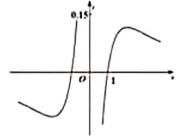
\includegraphics[width=.42\linewidth]{assets/asset-072-01.jpg}
\end{center}

\begin{center}
  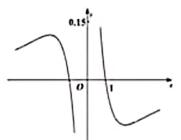
\includegraphics[width=.42\linewidth]{assets/asset-072-02.jpg}
\end{center}
\begin{choices}
  \item A
  \item B
  \item C
  \item D
\end{choices}
\begin{solution}
\textbf{答案：}B

\textbf{分析：}由函数为偶函数可排除 AC，再由当 $x \in (0,1)$ 时，$f(x) < 0$，排除 D，即可得解.

\textbf{详解：}设 $y = f(x) = \frac{\ln |x|}{x^2 + 2}$，定义域为 $\{ x | x \neq 0 \}$，关于原点对称，又 $f(-x) = \frac{\ln | -x |}{(-x)^2 + 2} = f(x)$，所以函数为偶函数，排除 AC；当 $x \in (0,1)$ 时，$\ln |x| < 0$，$x^2 + 2 > 0$，所以 $f(x) < 0$，排除 D. 故选：B.
\end{solution}
\end{question}

\begin{question}[points=5]
\textbf{来源：}2021 年 天津卷，第 5 题\par
设 $a = \log_2 0.3$，$b = \log_{\frac{1}{2}} 0.4$，$c = 0.4^{0.3}$，则 $a$，$b$，$c$ 的大小关系为（   ）
\begin{choices}
  \item $a < b < c$
  \item $c < a < b$
  \item $b < c < a$
  \item $a < c < b$
\end{choices}
\begin{solution}
\textbf{答案：}D

\textbf{分析：}根据指数函数和对数函数的性质求出 $a$，$b$，$c$ 的范围即可求解.

\textbf{详解：}$\because \log_2 0.3 < \log_2 1 = 0$，$\therefore a < 0$；$\because \log_{\frac{1}{2}} 0.4 = -\log_2 0.4 = \log_2 \frac{5}{2} > \log_2 2 = 1$，$\therefore b > 1$；$\because 0 < 0.4^{0.3} < 0.4^0 = 1$，$\therefore 0 < c < 1$；$\therefore a < c < b$. 故选：D.
\end{solution}
\end{question}

\begin{question}[points=5]
\textbf{来源：}2021 年 天津卷，第 7 题\par
若 $2^a = 5^b = 10$，则 $\frac{1}{a} + \frac{1}{b} =$（   ）
\begin{choices}
  \item $-1$
  \item $\lg 7$
  \item $1$
  \item $\log_{7} 10$
\end{choices}
\begin{solution}
\textbf{答案：}C

\textbf{分析：}由已知表示出 $a$，$b$，再由换底公式可求.

\textbf{详解：}$\because 2^a = 5^b = 10$，$\therefore a = \log_2 10$，$b = \log_5 10$，$\therefore \frac{1}{a} + \frac{1}{b} = \frac{1}{\log_2 10} + \frac{1}{\log_5 10} = \lg 2 + \lg 5 = \lg 10 = 1$．故选：C.
\end{solution}
\end{question}

\begin{question}[points=5]
\textbf{来源：}2021 年 天津卷，第 9 题\par
设 $a \in \mathbb{R}$，函数 $f(x) = \begin{cases} \cos(2\pi x - 2\pi a), & x < a \\ x^2 - 2(a+1)x + a^2 + 5, & x \ge a \end{cases}$，若 $f(x)$ 在区间 $(0, +\infty)$ 内恰有6个零点，则 $a$ 的取值范围是（   ）
\begin{choices}
  \item $\left(2, \frac{9}{4}\right] \cup \left(\frac{5}{2}, \frac{11}{4}\right]$
  \item $\left(\frac{7}{4}, 2\right) \cup \left(\frac{5}{2}, \frac{11}{4}\right)$
  \item $\left(2, \frac{9}{4}\right] \cup \left[\frac{11}{4}, 3\right)$
  \item $\left(\frac{7}{4}, 2\right) \cup \left[\frac{11}{4}, 3\right)$
\end{choices}
\begin{solution}
\textbf{答案：}A

\textbf{分析：}由 $x^2 - 2(a+1)x + a^2 + 5 = 0$ 最多有2个根，可得 $\cos(2\pi x - 2\pi a)=0$ 至少有4个根，分别讨论当 $x < a$ 和 $x \ge a$ 时两个函数零点个数情况，再结合考虑即可得出.

\textbf{详解：}略
\end{solution}
\end{question}

\begin{question}[points=5]
\textbf{来源：}2021 年 新高考II卷，第 7 题\par
已知$a=\log_5 2$，$b=\log_8 3$，$c=\frac{1}{2}$，则下列判断正确的是（ ）
\begin{choices}
  \item A. $c<b<a$
  \item B. $b<a<c$
  \item C. $a<c<b$
  \item D. $a<b<c$
\end{choices}
\begin{solution}
\textbf{答案：}C

\textbf{分析：}对数函数的单调性可比较$a$、$b$与$c$的大小关系，由此可得出结论.

\textbf{详解：}$a=\log_5 2<\log_5 \sqrt{5}=\frac{1}{2}=\log_8 2\sqrt{2}<\log_8 3=b$，即$a<c<b$.故选：C.
\end{solution}
\end{question}

\begin{question}[points=5]
\textbf{来源：}2021 年 新高考II卷，第 8 题\par
已知函数$f(x)$的定义域为$\mathbb{R}$，$f(x+2)$为偶函数，$f(2x+1)$为奇函数，则（ ）
\begin{choices}
  \item A. $f(-\frac{1}{2})=0$
  \item B. $f(-1)=0$
  \item C. $f(2)=0$
  \item D. $f(4)=0$
\end{choices}
\begin{solution}
\textbf{答案：}B

\textbf{分析：}推导出函数$f(x)$是以4为周期的周期函数，由已知条件得出$f(1)=0$，结合已知条件可得出结论.

\textbf{详解：}因为函数$f(x+2)$为偶函数，则$f(2+x)=f(2-x)$，可得$f(x+3)=f(1-x)$，因为函数$f(2x+1)$为奇函数，则$f(1-2x)=-f(2x+1)$，所以$f(1-x)=-f(x+1)$，所以$f(x+3)=-f(x+1)=f(x-1)$，即$f(x)=f(x+4)$，故函数$f(x)$是以4为周期的周期函数，因为函数$F(x)=f(2x+1)$为奇函数，则$F(0)=f(1)=0$，故$f(-1)=-f(1)=0$，其它三个选项未知.故选：B.
\end{solution}
\end{question}

\begin{question}[points=5]
\textbf{来源：}2021 年 新高考II卷，第 14 题；次专题：导数\par
写出一个同时具有下列性质①②③的函数$f(x)$: ．

① $f(x_1x_2)=f(x_1)f(x_2)$；②当$x\in(0,+\infty)$时，$f'(x)>0$；③ $f'(x)$是奇函数．
\fillin[{$f(x)=x^4$（答案不唯一，$f(x)=x^{2n}(n\in\mathbb{N}^*)$均满足）}]
\begin{solution}
\textbf{答案：}$f(x)=x^4$（答案不唯一，$f(x)=x^{2n}(n\in\mathbb{N}^*)$均满足）

\textbf{分析：}根据幂函数的性质可得所求的$f(x)$.

\textbf{详解：}取$f(x)=x^4$，则$f(x_1x_2)=(x_1x_2)^4=x_1^4x_2^4=f(x_1)f(x_2)$，满足①，$f'(x)=4x^3$，$x>0$时有$f'(x)>0$，满足②，$f'(x)=4x^3$的定义域为$\mathbb{R}$，又$f'(-x)=-4x^3=-f'(x)$，故$f'(x)$是奇函数，满足③.故答案为：$f(x)=x^4$（答案不唯一，$f(x)=x^{2n}(n\in\mathbb{N}^*)$均满足）.
\end{solution}
\end{question}

\begin{question}[points=5]
\textbf{来源：}2021 年 新高考I卷，第 13 题\par
已知函数 $f(x) = x^3(a \cdot 2^x - 2^{-x})$ 是偶函数, 则 $a =$ .
\fillin[{$1$}]
\begin{solution}
\textbf{答案：}$1$

\textbf{分析：}利用偶函数的定义可求参数 $a$ 的值.

\textbf{详解：}因为 $f(x) = x^3(a \cdot 2^x - 2^{-x})$, 故 $f(-x) = -x^3(a \cdot 2^{-x} - 2^x)$. 由 $f(-x) = f(x)$ 得 $x^3(a \cdot 2^x - 2^{-x}) = -x^3(a \cdot 2^{-x} - 2^x)$, 整理得 $(a-1)(2^x + 2^{-x}) = 0$, 所以 $a = 1$.
\end{solution}
\end{question}

\begin{question}[points=5]
\textbf{来源：}2021 年 新高考I卷，第 15 题\par
函数 $f(x) = |2x - 1| - 2\ln x$ 的最小值为.
\fillin[{$1$}]
\begin{solution}
\textbf{答案：}$1$

\textbf{分析：}由解析式知定义域为 $(0, +\infty)$, 分段讨论并利用导数研究单调性, 求最小值.

\textbf{详解：}定义域 $(0, +\infty)$. 当 $0 < x \leq \frac{1}{2}$ 时, $f(x) = 1 - 2x - 2\ln x$, 单调递减; 当 $\frac{1}{2} < x \leq 1$ 时, $f(x) = 2x - 1 - 2\ln x$, $f'(x) = 2 - \frac{2}{x} \leq 0$, 递减; 当 $x > 1$ 时, $f(x) = 2x - 1 - 2\ln x$, $f'(x) = 2 - \frac{2}{x} > 0$, 递增. 故 $f(x)$ 在 $(0,1]$ 递减, 在 $[1, +\infty)$ 递增, 最小值为 $f(1) = 1$.
\end{solution}
\end{question}

\begin{question}[points=4]
\textbf{来源：}2021 年 浙江卷，第 7 题\par
已知函数 $f(x) = x^2 + \frac{1}{4}$, $g(x) = \sin x$, 则图象为如图的函数可能是（   ）
\begin{choices}
  \item $y = f(x) + g(x) - \frac{1}{4}$
  \item $y = f(x) - g(x) - \frac{1}{4}$
  \item $y = f(x)g(x)$
  \item $y = \frac{g(x)}{f(x)}$
\end{choices}
\begin{solution}
\textbf{答案：}D

\textbf{分析：}由函数的奇偶性可排除 A、B, 结合导数判断函数的单调性可判断 C, 即可得解.

\textbf{详解：}A 非奇非偶, 排除；B 非奇非偶, 排除；C 求导在 $x=\frac{\pi}{4}$ 处导数为正, 与图象不符, 排除. 故选 D.
\end{solution}
\end{question}

\begin{question}[points=4]
\textbf{来源：}2021 年 浙江卷，第 12 题\par
已知 $a\in\mathbb{R}$, 函数 $f(x)=\begin{cases} x^2-4, & x>2 \\ |x-3|+a, & x\leq 2 \end{cases}$, 若 $f[f(\sqrt{6})]=3$, 则 $a=$ .
\fillin[{$2$}]
\begin{solution}
\textbf{答案：}$2$

\textbf{分析：}由题意结合函数的解析式得到关于 $a$ 的方程, 解方程可得 $a$ 的值.

\textbf{详解：}$f(\sqrt{6}) = (\sqrt{6})^2-4=2$, 则 $f[f(\sqrt{6})]=f(2)=|2-3|+a=1+a=3$, 所以 $a=2$.
\end{solution}
\end{question}

\section*{2022 年}

\begin{question}[points=4]
\textbf{来源：}2022 年 北京卷，第 4 题\par
已知函数 $f(x) = \dfrac{1}{1+2^x}$，则对任意实数 $x$，有
\begin{choices}
  \item $f(-x) + f(x) = 0$
  \item $f(-x) - f(x) = 0$
  \item $f(-x) + f(x) = 1$
  \item $f(-x) - f(x) = \dfrac{1}{3}$
\end{choices}
\begin{solution}
\textbf{答案：}C

\textbf{分析：}直接代入计算，注意通分。

\textbf{详解：}$f(-x) + f(x) = \dfrac{1}{1+2^{-x}} + \dfrac{1}{1+2^x} = \dfrac{2^x}{1+2^x} + \dfrac{1}{1+2^x} = 1$，故A错误，C正确；$f(-x) - f(x) = \dfrac{1}{1+2^{-x}} - \dfrac{1}{1+2^x} = \dfrac{2^x}{1+2^x} - \dfrac{1}{1+2^x} = \dfrac{2^x-1}{2^x+1} = 1 - \dfrac{2}{2^x+1}$，不是常数，故BD错误。故选C。
\end{solution}
\end{question}

\begin{question}[points=4]
\textbf{来源：}2022 年 北京卷，第 7 题\par
在北京冬奥会上，国家速滑馆“冰丝带”使用高效环保的二氧化碳跨临界直冷制冰技术，为实现绿色冬奥作出了贡献。如图描述了一定条件下二氧化碳所处的状态与 $T$ 和 $\lg P$ 的关系，其中 $T$ 表示温度，单位是 $K$；$P$ 表示压强，单位是 $bar$。下列结论中正确的是
\begin{choices}
  \item 当 $T = 220$，$P = 1026$ 时，二氧化碳处于液态
  \item 当 $T = 270$，$P = 128$ 时，二氧化碳处于气态
  \item 当 $T = 300$，$P = 9987$ 时，二氧化碳处于超临界状态
  \item 当 $T = 360$，$P = 729$ 时，二氧化碳处于超临界状态
\end{choices}
\begin{solution}
\textbf{答案：}D

\textbf{分析：}根据 $T$ 与 $\lg P$ 的关系图可得正确的选项。

\textbf{详解：}当 $T = 220$，$P = 1026$ 时，$\lg P > 3$，此时二氧化碳处于固态，故A错误。
当 $T = 270$，$P = 128$ 时，$2 < \lg P < 3$，此时二氧化碳处于液态，故B错误。
当 $T = 300$，$P = 9987$ 时，$\lg P$ 与4非常接近，故此时二氧化碳处于固态，且 $T=300$ 时对应的是非超临界状态，故C错误。
当 $T = 360$，$P = 729$ 时，因 $2 < \lg P < 3$，故此时二氧化碳处于超临界状态，故D正确。故选D。
\end{solution}
\end{question}

\begin{question}[points=5]
\textbf{来源：}2022 年 北京卷，第 11 题\par
函数 $f(x) = \dfrac{1}{x} + \sqrt{1-x}$ 的定义域是。
\fillin[{$(-\infty,0) \cup (0,1]$}]
\begin{solution}
\textbf{答案：}$(-\infty,0) \cup (0,1]$

\textbf{分析：}根据偶次方根的被开方数非负、分母不为零得到方程组，解得即可。

\textbf{详解：}解：因为 $f(x) = \dfrac{1}{x} + \sqrt{1-x}$，所以 $\begin{cases} 1-x \geq 0 \\ x \neq 0 \end{cases}$，解得 $x \leq 1$ 且 $x \neq 0$，故函数的定义域为 $(-\infty,0) \cup (0,1]$。
\end{solution}
\end{question}

\begin{question}[points=5]
\textbf{来源：}2022 年 北京卷，第 14 题\par
设函数 $f(x) = \begin{cases} -ax+1, & x < a \\ (x-2)^2, & x \geq a \end{cases}$ 若 $f(x)$ 存在最小值，则 $a$ 的一个取值为；$a$ 的最大值为。
\fillin[{$0$（答案不唯一）；$1$}]
\begin{solution}
\textbf{答案：}$0$（答案不唯一）；$1$

\textbf{分析：}根据分段函数中的函数 $y = -ax+1$ 的单调性进行分类讨论，可知 $a=0$ 符合条件，$a<0$ 不符合条件，$a>0$ 时函数 $y=-ax+1$ 没有最小值，故 $f(x)$ 的最小值只能取 $y=(x-2)^2$ 的最小值，根据定义域讨论可得。

\textbf{详解：}解：若 $a=0$ 时，$f(x)=\begin{cases} 1, & x<0 \\ (x-2)^2, & x\geq 0 \end{cases}$，$\therefore f(x)_{\min}=0$；若 $a<0$ 时，当 $x<a$ 时，$f(x)=-ax+1$ 单调递增，当 $x\to -\infty$ 时，$f(x)\to -\infty$，故 $f(x)$ 没有最小值；若 $a>0$ 时，当 $x<a$ 时，$f(x)=-ax+1$ 单调递减，$f(x) > f(a) = -a^2+1$，当 $x\geq a$ 时，$f(x)_{\min}=\begin{cases} 0 & (0<a<2) \\ (a-2)^2 & (a\geq 2) \end{cases}$，$\therefore -a^2+1\geq 0$ 或 $-a^2+1\geq (a-2)^2$，解得 $0<a\leq 1$。综上可得 $0\leq a\leq 1$，故 $a$ 的一个取值为0（答案不唯一），$a$ 的最大值为1。
\end{solution}
\end{question}

\begin{question}[points=5]
\textbf{来源：}2022 年 全国甲卷-理科，第 5 题\par
函数 $y=(3^x-3^{-x})\cos x$ 在区间 $\left[-\frac{\pi}{2}, \frac{\pi}{2}\right]$ 的图象大致为（ ）

\begin{center}
  
\includegraphics[width=.42\linewidth]{assets/asset-087-01.jpg}
\end{center}
\begin{choices}
  \item A选项图
  \item B选项图
  \item C选项图
  \item D选项图
\end{choices}
\begin{solution}
\textbf{答案：}A

\textbf{分析：}由函数的奇偶性结合指数函数、三角函数的性质逐项排除即可得解.

\textbf{详解：}令 $f(x)=(3^x-3^{-x})\cos x$, $x\in\left[-\frac{\pi}{2},\frac{\pi}{2}\right]$, 则 $f(-x)=(3^{-x}-3^x)\cos(-x)=-(3^x-3^{-x})\cos x=-f(x)$, 所以 $f(x)$ 为奇函数，排除BD；又当 $x\in\left(0,\frac{\pi}{2}\right)$ 时，$3^x-3^{-x}>0$, $\cos x>0$, 所以 $f(x)>0$, 排除C. 故选A.
\end{solution}
\end{question}

\begin{question}[points=5]
\textbf{来源：}2022 年 全国甲卷-文科，第 7 题\par
函数 $f(x)=\left(3^x-3^{-x}\right)\cos x$ 在区间 $\left[-\frac{\pi}{2},\frac{\pi}{2}\right]$ 的图像大致为

\begin{center}
  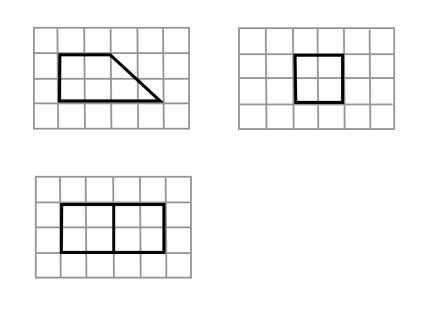
\includegraphics[width=.42\linewidth]{assets/asset-088-01.jpg}
\end{center}
\begin{choices}
  \item A．
  \item B．
  \item C．
  \item D．
\end{choices}
\begin{solution}
\textbf{答案：}A
\end{solution}
\end{question}

\begin{question}[points=5]
\textbf{来源：}2022 年 全国甲卷-文科，第 12 题\par
已知 $9^m=10, a=10^m-11, b=8^m-9$，则
\begin{choices}
  \item $a>0>b$
  \item $a>b>0$
  \item $b>a>0$
  \item $b>0>a$
\end{choices}
\begin{solution}
\textbf{答案：}A
\end{solution}
\end{question}

\begin{question}[points=5]
\textbf{来源：}2022 年 全国乙卷-理科，第 12 题\par
已知函数$f(x), g(x)$的定义域均为$\mathbb{R}$，且$f(x) + g(2-x) = 5$，$g(x) - f(x-4) = 7$．若$y = g(x)$的图像关于直线$x=2$对称，$g(2) = 4$，则$\sum\limits_{k=1}^{22} f(k) =$（\qquad）
\begin{choices}
  \item $-21$
  \item $-22$
  \item $-23$
  \item $-24$
\end{choices}
\begin{solution}
\textbf{答案：}D

\textbf{分析：}根据对称性和已知条件得到$f(x) + f(x-2) = -2$，从而得到$f(3)+f(5)+\cdots+f(21) = -10$，$f(4)+f(6)+\cdots+f(22) = -10$，然后根据条件得到$f(2)$的值，再由题意得到$g(3)=6$从而得到$f(1)$的值即可求解.

\textbf{详解：}因为$y=g(x)$的图像关于直线$x=2$对称，所以$g(2-x) = g(x+2)$，因为$g(x) - f(x-4) = 7$，所以$g(x+2) - f(x-2) = 7$，即$g(x+2) = 7 + f(x-2)$，因为$f(x) + g(2-x) = 5$，所以$f(x) + g(x+2) = 5$，代入得$f(x) + [7 + f(x-2)] = 5$，即$f(x) + f(x-2) = -2$，所以$f(3)+f(5)+\cdots+f(21) = (-2)\times5 = -10$，\\$f(4)+f(6)+\cdots+f(22) = (-2)\times5 = -10$，因为$f(x) + g(2-x) = 5$，所以$f(0) + g(2) = 5$，即$f(0) = 1$，所以$f(2) = -2 - f(0) = -3$，因为$g(x) - f(x-4) = 7$，所以$g(x+4) - f(x) = 7$，又因为$f(x) + g(2-x) = 5$，联立得，$g(2-x) + g(x+4) = 12$，所以$y=g(x)$的图像关于点$(3,6)$中心对称，因为函数$g(x)$的定义域为$\mathbb{R}$，所以$g(3)=6$因为$f(x) + g(x+2) = 5$，所以$f(1) = 5 - g(3) = -1$，所以$\sum\limits_{k=1}^{22} f(k) = f(1)+f(2)+[f(3)+f(5)+\cdots+f(21)]+[f(4)+f(6)+\cdots+f(22)] = -1 -3 -10 -10 = -24$.
\end{solution}
\end{question}

\begin{question}[points=5]
\textbf{来源：}2022 年 全国乙卷-文科，第 8 题\par
如图是下列四个函数中的某个函数在区间 $[-3,3]$ 的大致图像，则该函数是
\begin{choices}
  \item $y=\frac{-x^3+3x}{x^2+1}$
  \item $y=\frac{x^3-x}{x^2+1}$
  \item $y=\frac{2x\cos x}{x^2+1}$
  \item $y=\frac{2\sin x}{x^2+1}$
\end{choices}
\begin{solution}
\textbf{答案：}A

\textbf{分析：}由函数图像的特征结合函数的性质逐项排除即可得解.

\textbf{详解：}设 $f(x)=\frac{x^3-x}{x^2+1}$, 则 $f(1)=0$, 排除B. 设 $h(x)=\frac{2x\cos x}{x^2+1}$, 当 $x\in(0,\frac{\pi}{2})$ 时 $0<\cos x<1$, 则 $h(x)<\frac{2x}{x^2+1}\le 1$, 排除C. 设 $g(x)=\frac{2\sin x}{x^2+1}$, 则 $g(3)=\frac{2\sin3}{10}>0$, 排除D. 故选A.
\end{solution}
\end{question}

\begin{question}[points=5]
\textbf{来源：}2022 年 全国乙卷-文科，第 16 题\par
若 $f(x) = \ln\left| a + \frac{1}{1-x} \right| + b$ 是奇函数，则 $a=$ , $b=$ .
\fillin[{$a=-\frac12$, $b=\ln2$}]
\begin{solution}
\textbf{答案：}$a=-\frac12$, $b=\ln2$

\textbf{分析：}根据奇函数的定义即可求出.

\textbf{详解：}由奇函数定义域关于原点对称，得 $a=-\frac12$, 再由 $f(0)=0$ 得 $b=\ln2$. 经检验，$f(x)=\ln\left|\frac{1+x}{1-x}\right|$ 满足奇函数.
\end{solution}
\end{question}

\begin{question}[points=14]
\textbf{来源：}2022 年 上海卷，第 2 题\par
$f(x)=\log_3(x+a)+\log_3(6-x)$．

（1）若将函数$f(x)$图像向下移$m(m>0)$后，图像经过$(3,0)$，$(5,0)$，求实数$a$，$m$的值．

（2）若$a>-3$且$a\neq0$，求解不等式$f(x)\leq f(6-x)$．
\begin{solution}
\textbf{答案：}（1）$a=-2,m=1$（2）当$-3<a<0$时，解集为$(-a,3]$；当$a>0$时，解集为$[3,6)$

\textbf{分析：}（1）写出函数图像下移$m$个单位后的解析式，把点的坐标代入求解即可得出$a$和$m$的值．（2）不等式化为$\log_3(x+a)+\log_3(6-x)\leq \log_3(x+6-x)+\log_3 a$，写出等价不等式组，求出解集即可．

\textbf{详解：}解：（1）因为函数$f(x)=\log_3(x+a)+\log_3(6-x)$，将函数$f(x)$图像向下移$m(m>0)$后，得$y=f(x)-m=\log_3(x+a)+\log_3(6-x)-m$的图像，由函数图像经过点$(3,0)$和$(5,0)$，所以$\begin{cases}\log_3(3+a)+1-m=0\\\log_3(5+a)+0-m=0\end{cases}$，解得$a=-2$，$m=1$．（2）$a>-3$且$a\neq0$时，不等式$f(x)\leq f(6-x)$可化为$\log_3(x+a)+\log_3(6-x)\leq \log_3(x+6-x)+\log_3 a$，等价于$\begin{cases}x+a>0\\6-x>0\\x+6-x>0\\a>0\\(x+a)(6-x)\leq a(x+6-x)\end{cases}$即$\begin{cases}x>-a\\x<6\\x<6\\a>0\\(x+a)(6-x)\leq 6a\end{cases}$，解得$\begin{cases}x>-a\\x<6\\a>0\\x(x-3)\geq0\end{cases}$，当$-3<a<0$时，$0<-a<3$，$3<a+6<6$，解不等式得$-a<x\leq 3$，当$a>0$时，$-a<0$，$a+6>6$，解不等式得$3\leq x<6$；综上知，$-3<a<0$时，不等式$f(x)\leq f(6-x)$的解集是$(-a,3]$，$a>0$时，不等式$f(x)\leq f(6-x)$的解集是$[3,6)$．
\end{solution}
\end{question}

\begin{question}[points=5]
\textbf{来源：}2022 年 上海卷，第 7 题\par
若函数$f(x)=\begin{cases} x^2(x-1), & x<0 \\ x+a, & x>0 \\ 0, & x=0 \end{cases}$，为奇函数，求参数$a$的值为 ．
\fillin[{$1$}]
\begin{solution}
\textbf{答案：}$1$

\textbf{分析：}利用奇函数的定义可得$f(-x)=-f(x)$，故有$f(-1)=-f(1)$，由此求得$a$的值．

\textbf{详解：}解：因为 函数$f(x)$为奇函数，所以 $f(-x)=-f(x)$，所以 $f(-1)=-f(1)$，所以 $-(1^2-1)=-(1+a)$，即$0=-(1+a)$，解得$a=-1$，但验证当$a=-1$时，$f(x)$不是奇函数，故舍去；再考虑$f(0)=0$成立，由$f(-1)=-f(1)$得$a=1$，检验当$a=1$时，$f(x)=\begin{cases} x^2(x-1), & x<0 \\ x+1, & x>0 \\ 0, & x=0 \end{cases}$是奇函数，故$a=1$．故答案为：$1$．
\end{solution}
\end{question}

\begin{question}[points=5]
\textbf{来源：}2022 年 上海卷，第 11 题\par
设函数$f(x)$满足$f(x)=\frac{1}{f(x)+1}$对任意$x\in[0,+\infty)$都成立，其值域是$A$，已知对任何满足上述条件的$f(x)$都有$\{y|y=f(t),0\leq t\leq a\}=A$，则$a$的取值范围为 ．
\fillin[{$[\frac{\sqrt{5}-1}{2},+\infty)$}]
\begin{solution}
\textbf{答案：}$[\frac{\sqrt{5}-1}{2},+\infty)$

\textbf{分析：}由题可得$\{y|y=f(t),0\leq t\leq \frac{\sqrt{5}-1}{2}\}=A$，再根据$a<\frac{\sqrt{5}-1}{2}$时不合题意，进而即得；或等价于$\frac{1}{1+a+x}\leq a$恒成立，即$\frac{1}{a}-1\leq x$恒成立，进而即得．

\textbf{详解：}解：法一：令$x=\frac{1}{x+1}$，解得$x=\frac{\sqrt{5}-1}{2}$（负值舍去），当$x_1\in[0,\frac{\sqrt{5}-1}{2})$时，$x_2=\frac{1}{x_1+1}\in(\frac{\sqrt{5}-1}{2},1]$，当$x_1\in(\frac{\sqrt{5}-1}{2},+\infty)$时，$x_2=\frac{1}{x_1+1}\in(0,\frac{\sqrt{5}-1}{2})$，且当$x_1\in(\frac{\sqrt{5}-1}{2},+\infty)$时，总存在$x_2=\frac{1}{x_1+1}\in(0,\frac{\sqrt{5}-1}{2})$，使得$f(x_1)=f(x_2)$，故$\{y|y=f(t),0\leq t\leq \frac{\sqrt{5}-1}{2}\}=A$，若$a<\frac{\sqrt{5}-1}{2}$，易得$\frac{\sqrt{5}-1}{2}\notin\{y|y=f(t),0\leq t\leq a\}$，所以$a\geq\frac{\sqrt{5}-1}{2}$，即实数$a$的取值范围为$[\frac{\sqrt{5}-1}{2},+\infty)$；法二：原命题等价于任意$x>0$，$f(a+x)=\frac{1}{1+a+x}\leq a$恒成立，所以$a\geq\frac{1}{a}-1$，即$a^2+a-1\geq0$，解得$a\geq\frac{\sqrt{5}-1}{2}$或$a\leq\frac{-\sqrt{5}-1}{2}$（舍），所以$a\in[\frac{\sqrt{5}-1}{2},+\infty)$．故答案为：$[\frac{\sqrt{5}-1}{2},+\infty)$．
\end{solution}
\end{question}

\begin{question}[points=5]
\textbf{来源：}2022 年 上海卷，第 12 题\par
（第 12 题缺失，原卷无对应内容）
\fillin[{$$}]
\begin{solution}
\end{solution}
\end{question}

\begin{question}[points=5]
\textbf{来源：}2022 年 天津卷，第 3 题\par
函数 $f(x)=\frac{x^2-1}{x}$ 的图像为（   ）

\begin{center}
  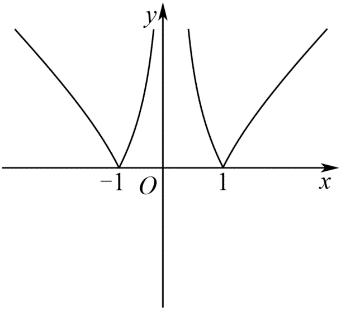
\includegraphics[width=.42\linewidth]{assets/asset-097-01.jpg}
\end{center}
\begin{choices}
  \item A
  \item B
  \item C
  \item D
\end{choices}
\begin{solution}
\textbf{答案：}D

\textbf{分析：}分析函数 $f(x)$ 的定义域、奇偶性、单调性及其在 $(-\infty,0)$ 上的函数值符号，结合排除法可得出合适的选项. 函数 $f(x)=\frac{x^2-1}{x}$ 的定义域为 $\{x\mid x\ne 0\}$，且 $f(-x)=\frac{(-x)^2-1}{-x}=-\frac{x^2-1}{x}=-f(x)$，函数为奇函数，A 选项错误；又当 $x<0$ 时，$f(x)=\frac{x^2-1}{x}\le 0$，C 选项错误；当 $x>1$ 时，$f(x)=\frac{x^2-1}{x}=x-\frac{1}{x}$ 单调递增，故 B 选项错误；故选 D.
\end{solution}
\end{question}

\begin{question}[points=5]
\textbf{来源：}2022 年 天津卷，第 5 题\par
已知 $a=2^{0.7}$，$b=\left(\frac{1}{3}\right)^{0.7}$，$c=\log_2\frac{1}{3}$，则（   ）
\begin{choices}
  \item $a>c>b$
  \item $b>c>a$
  \item $a>b>c$
  \item $c>a>b$
\end{choices}
\begin{solution}
\textbf{答案：}C

\textbf{分析：}因为 $2^{0.7}>\left(\frac{1}{3}\right)^{0.7}>0=\log_2 1>\log_2\frac{1}{3}$，故 $a>b>c$.
\end{solution}
\end{question}

\begin{question}[points=5]
\textbf{来源：}2022 年 天津卷，第 6 题\par
化简 $(2\log_4 3+\log_8 3)(\log_3 2+\log_9 2)$ 的值为（   ）
\begin{choices}
  \item 1
  \item 2
  \item 4
  \item 6
\end{choices}
\begin{solution}
\textbf{答案：}2

\textbf{分析：}原式 $=(2\times\frac{1}{2}\log_2 3+\frac{1}{3}\log_2 3)(\log_3 2+\frac{1}{2}\log_3 2)=(\frac{4}{3}\log_2 3)\times(\frac{3}{2}\log_3 2)=2$.
\end{solution}
\end{question}

\begin{question}[points=5]
\textbf{来源：}2022 年 天津卷，第 15 题\par
设 $a\in\mathbb{R}$，对任意实数 $x$，记 $f(x)=\min\{|x-2|, x^2-ax+3a-5\}$．若 $f(x)$ 至少有 3 个零点，则实数 $a$ 的取值范围为.
\fillin[{$[10,+\infty)$}]
\begin{solution}
\textbf{答案：}$[10,+\infty)$

\textbf{分析：}设 $g(x)=x^2-ax+3a-5$，$h(x)=|x-2|$，由 $h(x)=0$ 可得 $x=\pm2$。要使得 $f(x)$ 至少有3个零点，则 $g(x)$ 至少有一个零点，即 $\Delta=a^2-12a+20\ge0$，解得 $a\le2$ 或 $a\ge10$。①当 $a=2$ 时，$g(x)=x^2-2x+1$，只有两个零点，不合；②当 $a<2$ 时，设 $g(x)$ 的两个零点为 $x_1<x_2$，要使得 $f(x)$ 至少有3个零点，则 $x_2\le-2$，由韦达定理 $\frac{a}{2}<-2$ 且 $g(-2)=4+5a-5\ge0$，无解；③当 $a=10$ 时，$g(x)=x^2-10x+25$，有3个零点，合；④当 $a>10$ 时，设 $g(x)$ 的两个零点为 $x_3<x_4$，要使得 $f(x)$ 至少有3个零点，则 $x_3\ge2$，即 $\frac{a}{2}>2$ 且 $g(2)=4+a-5\ge0$，解得 $a>10$。综上，$a\in[10,+\infty)$.
\end{solution}
\end{question}

\begin{question}[points=5]
\textbf{来源：}2022 年 新高考II卷，第 8 题\par
已知函数$f(x)$的定义域为$\mathbf{R}$，且$f(x+y)+f(x-y)=f(x)f(y),f(1)=1$，则$\displaystyle\sum_{k=1}^{22}f(k)=$（ ）
\begin{choices}
  \item $-3$
  \item $-2$
  \item $0$
  \item $1$
\end{choices}
\begin{solution}
\textbf{答案：}$-3$

\textbf{分析：}根据题意赋值即可知函数$f(x)$的一个周期为6，求出函数一个周期中的$f(1),f(2),\cdots,f(6)$的值，即可解出.

\textbf{详解：}因为$f(x+y)+f(x-y)=f(x)f(y)$，令$x=1,y=0$可得$2f(1)=f(1)f(0)$，所以$f(0)=2$，令$x=0$可得$f(y)+f(-y)=2f(y)$，即$f(y)=f(-y)$，所以函数$f(x)$为偶函数，令$y=1$得$f(x+1)+f(x-1)=f(x)f(1)=f(x)$，即有$f(x+2)+f(x)=f(x+1)$，从而可知$f(x+2)=-f(x-1)$，$f(x-1)=-f(x-4)$，故$f(x+2)=f(x-4)$，即$f(x)=f(x+6)$，所以函数$f(x)$的一个周期为6. 因为$f(2)=f(1)-f(0)=1-2=-1$，$f(3)=f(2)-f(1)=-1-1=-2$，$f(4)=f(-2)=f(2)=-1$，$f(5)=f(-1)=f(1)=1$，$f(6)=f(0)=2$，所以一个周期内的$f(1)+f(2)+\cdots+f(6)=0$．由于22除以6余4，所以$\sum_{k=1}^{22}f(k)=f(1)+f(2)+f(3)+f(4)=1-1-2-1=-3$，故选A.
\end{solution}
\end{question}

\begin{question}[points=5]
\textbf{来源：}2022 年 新高考I卷，第 7 题\par
设 $a = 0.1e^{0.1}$, $b = \frac{1}{9}$, $c = -\ln 0.9$, 则
\begin{choices}
  \item $a < b < c$
  \item $c < b < a$
  \item $c < a < b$
  \item $a < c < b$
\end{choices}
\begin{solution}
\textbf{答案：}C

\textbf{分析：}构造函数 $f(x) = \ln(1+x) - x$, 利用导数判断其单调性, 由此确定 $a, b, c$ 的大小.

\textbf{详解：}设 $f(x) = \ln(1+x) - x\ (x > -1)$, 因为 $f'(x) = \frac{1}{1+x} - 1 = -\frac{x}{1+x}$, 当 $x \in (-1, 0)$ 时, $f'(x) > 0$, 当 $x \in (0, +\infty)$ 时 $f'(x) < 0$. 所以函数 $f(x) = \ln(1+x) - x$ 在 $(0, +\infty)$ 单调递减, 在 $(-1, 0)$ 上单调递增. 所以 $f(\frac{1}{9}) < f(0) = 0$, 所以 $\ln\frac{10}{9} - \frac{1}{9} < 0$, 故 $\frac{1}{9} > \ln\frac{10}{9} = -\ln 0.9$, 即 $b > c$. 所以 $f(-\frac{1}{10}) < f(0) = 0$, 所以 $\ln\frac{9}{10} + \frac{1}{10} < 0$, 故 $\frac{1}{10} < \ln\frac{10}{9}$, 所以 $e^{-\frac{1}{10}} < \frac{9}{10}$, 即 $e^{0.1} < \frac{10}{9}$, 故 $0.1e^{0.1} < \frac{1}{9}$, 即 $a < b$. 设 $g(x) = xe^x + \ln(1-x)\ (0 < x < 1)$, 则 $g'(x) = (x+1)e^x + \frac{-1}{1-x} = \frac{(x-1)e^x + 1}{x-1}$. 令 $h(x) = e^x(x^2-1)+1$, $h'(x) = e^x(x^2+2x-1)$. 当 $0 < x < \sqrt{2}-1$ 时, $h'(x) < 0$, 函数 $h(x)$ 单调递减; 当 $\sqrt{2}-1 < x < 1$ 时, $h'(x) > 0$, 函数 $h(x)$ 单调递增. 又 $h(0)=0$, 所以当 $0 < x < \sqrt{2}-1$ 时, $h(x) < 0$, 所以 $g'(x) > 0$, 函数 $g(x)$ 单调递增. 所以 $g(0.1) > g(0)=0$, 即 $0.1e^{0.1} > -\ln 0.9$, 所以 $a > c$. 综上, $c < a < b$.
\end{solution}
\end{question}

\begin{question}[points=5]
\textbf{来源：}2022 年 新高考I卷，第 10 题\par
已知函数 $f(x) = x^3 - x + 1$, 则
\begin{choices}
  \item $f(x)$ 有两个极值点
  \item $f(x)$ 有三个零点
  \item 点 $(0,1)$ 是曲线 $y = f(x)$ 的对称中心
  \item 直线 $y = 2x$ 是曲线 $y = f(x)$ 的切线
\end{choices}
\begin{solution}
\textbf{答案：}AC

\textbf{分析：}利用极值点的定义可判断 A, 结合 $f(x)$ 的单调性、极值可判断 B, 利用平移可判断 C; 利用导数的几何意义判断 D.

\textbf{详解：}由题, $f'(x) = 3x^2 - 1$, 令 $f'(x) > 0$ 得 $x > \frac{\sqrt{3}}{3}$ 或 $x < -\frac{\sqrt{3}}{3}$, 令 $f'(x) < 0$ 得 $-\frac{\sqrt{3}}{3} < x < \frac{\sqrt{3}}{3}$. 所以 $f(x)$ 在 $(-\frac{\sqrt{3}}{3}, \frac{\sqrt{3}}{3})$ 上单调递减, 在 $(-\infty, -\frac{\sqrt{3}}{3})$, $(\frac{\sqrt{3}}{3}, +\infty)$ 上单调递增. 所以 $x = \pm\frac{\sqrt{3}}{3}$ 是极值点, 故 A 正确. 因为 $f(-\frac{\sqrt{3}}{3}) = 1 + \frac{2\sqrt{3}}{9} > 0$, $f(\frac{\sqrt{3}}{3}) = 1 - \frac{2\sqrt{3}}{9} > 0$, $f(-2) = -5 < 0$, 所以函数 $f(x)$ 在 $(-\infty, -\frac{\sqrt{3}}{3})$ 上有一个零点, 当 $x \ge \frac{\sqrt{3}}{3}$ 时, $f(x) \ge f(\frac{\sqrt{3}}{3}) > 0$, 即函数 $f(x)$ 在 $(\frac{\sqrt{3}}{3}, +\infty)$ 上无零点. 综上所述, 函数 $f(x)$ 有一个零点, 故 B 错误. 令 $h(x) = x^3 - x$, 该函数的定义域为 $\mathbb{R}$, $h(-x) = (-x)^3 - (-x) = -x^3 + x = -h(x)$, 则 $h(x)$ 是奇函数, $(0,0)$ 是 $h(x)$ 的对称中心. 将 $h(x)$ 的图象向上移动一个单位得到 $f(x)$ 的图象, 所以点 $(0,1)$ 是曲线 $y = f(x)$ 的对称中心, 故 C 正确. 令 $f'(x) = 3x^2 - 1 = 2$, 可得 $x = \pm 1$, 又 $f(1) = f(-1) = 1$. 当切点为 $(1,1)$ 时, 切线方程为 $y = 2x - 1$; 当切点为 $(-1,1)$ 时, 切线方程为 $y = 2x + 3$. 故 D 错误.
\end{solution}
\end{question}

\begin{question}[points=5]
\textbf{来源：}2022 年 新高考I卷，第 12 题；次专题：导数\par
已知函数 $f(x)$ 及其导函数 $f'(x)$ 的定义域均为 $\mathbb{R}$, 记 $g(x) = f'(x)$, 若 $f\left(\frac{3}{2} - 2x\right)$, $g(2 + x)$ 均为偶函数, 则
\begin{choices}
  \item $f(0) = 0$
  \item $g\left(-\frac{1}{2}\right) = 0$
  \item $f(-1) = f(4)$
  \item $g(-1) = g(2)$
\end{choices}
\begin{solution}
\textbf{答案：}BC

\textbf{分析：}转化题设条件为函数的对称性, 结合原函数与导函数图象的关系, 根据函数的性质逐项判断即可得解.

\textbf{详解：}因为 $f\left(\frac{3}{2} - 2x\right)$, $g(2 + x)$ 均为偶函数, 所以 $f\left(\frac{3}{2} - 2x\right) = f\left(\frac{3}{2} + 2x\right)$ 即 $f\left(\frac{3}{2} - x\right) = f\left(\frac{3}{2} + x\right)$, $g(2 + x) = g(2 - x)$. 所以 $f(3 - x) = f(x)$, $g(4 - x) = g(x)$, 则 $f(-1) = f(4)$, 故 C 正确. 函数 $f(x)$, $g(x)$ 的图象分别关于直线 $x = \frac{3}{2}$, $x = 2$ 对称. 又 $g(x) = f'(x)$, 且函数 $f(x)$ 可导, 所以 $g\left(\frac{3}{2}\right) = 0$, $g(3 - x) = -g(x)$. 所以 $g(4 - x) = g(x) = -g(3 - x)$, 所以 $g(x + 2) = -g(x + 1) = g(x)$. 所以 $g\left(-\frac{1}{2}\right) = g\left(\frac{3}{2}\right) = 0$, $g(-1) = g(1) = -g(2)$, 故 B 正确, D 错误. 若函数 $f(x)$ 满足题设条件, 则函数 $f(x) + C$ ($C$ 为常数) 也满足题设条件, 所以无法确定 $f(x)$ 的函数值, 故 A 错误.
\end{solution}
\end{question}

\begin{question}[points=4]
\textbf{来源：}2022 年 浙江卷，第 7 题\par
已知 $2^a = 5, \log_8 3 = b$，则 $4^{a-3b} =$ （ ）
\begin{choices}
  \item $25$
  \item $5$
  \item $\dfrac{25}{9}$
  \item $\dfrac{5}{3}$
\end{choices}
\begin{solution}
\textbf{答案：}C

\textbf{分析：}根据指数式与对数式的互化，幂的运算性质以及对数的运算性质即可解出．

\textbf{详解：}因为 $2^a = 5$，$b = \log_8 3 = \frac{1}{3} \log_2 3$，所以 $2^{3b} = 3$，则 $4^{a-3b} = \frac{4^a}{4^{3b}} = \frac{(2^a)^2}{(2^{3b})^2} = \frac{5^2}{3^2} = \frac{25}{9}$，故选C.
\end{solution}
\end{question}

\begin{question}[points=6]
\textbf{来源：}2022 年 浙江卷，第 14 题\par
已知函数 $f(x) = \begin{cases} -x^2+2, & x \le 1, \\ x+\dfrac{1}{x}-1, & x > 1, \end{cases}$ 则 $f\left(f\left(\frac{1}{2}\right)\right) =$ ；若当 $x \in [a,b]$ 时，$1 \le f(x) \le 3$，则 $b-a$ 的最大值是．
\fillin[{$\dfrac{37}{28}$；$3+\sqrt{3}$}]
\begin{solution}
\textbf{答案：}$\dfrac{37}{28}$；$3+\sqrt{3}$

\textbf{分析：}结合分段函数的解析式求函数值，由条件求出 $a$ 的最小值，$b$ 的最大值即可.

\textbf{详解：}$f(\frac{1}{2}) = -(\frac{1}{2})^2+2 = \frac{7}{4}$，$f(\frac{7}{4}) = \frac{7}{4}+\frac{4}{7}-1 = \frac{37}{28}$．当 $x\le1$ 时，由 $1\le -x^2+2 \le 3$ 得 $-1\le x\le1$；当 $x>1$ 时，由 $1\le x+\frac{1}{x}-1\le 3$ 得 $1<x\le 2+\sqrt{3}$；所以 $[a,b]\subseteq[-1,2+\sqrt{3}]$，$b-a$ 最大值为 $3+\sqrt{3}$.
\end{solution}
\end{question}

\section*{2023 年}

\begin{question}[points=4]
\textbf{来源：}2023 年 北京卷，第 4 题\par
下列函数中，在区间 $(0, +\infty)$ 上单调递增的是（ ）
\begin{choices}
  \item $f(x) = -\ln x$
  \item $f(x) = \dfrac{1}{2^x}$
  \item $f(x) = -\dfrac{1}{x}$
  \item $f(x) = 3^{|x-1|}$
\end{choices}
\begin{solution}
\textbf{答案：}C

\textbf{分析：}利用基本初等函数的单调性，结合复合函数的单调性判断 ABC，举反例排除 D 即可.

\textbf{详解：}对于 A，因为 $y=\ln x$ 在 $(0,+\infty)$ 上单调递增，$y=-x$ 在 $(0,+\infty)$ 上单调递减，所以 $f(x)=-\ln x$ 在 $(0,+\infty)$ 上单调递减，故 A 错误；对于 B，因为 $y=2^x$ 在 $(0,+\infty)$ 上单调递增，$y=\frac{1}{x}$ 在 $(0,+\infty)$ 上单调递减，所以 $f(x)=\frac{1}{2^x}$ 在 $(0,+\infty)$ 上单调递减，故 B 错误；对于 C，因为 $y=\frac{1}{x}$ 在 $(0,+\infty)$ 上单调递减，$y=-x$ 在 $(0,+\infty)$ 上单调递减，所以 $f(x)=-\frac{1}{x}$ 在 $(0,+\infty)$ 上单调递增，故 C 正确；对于 D，因为 $f(\frac{1}{2})=3^{-\frac{1}{2}}=\frac{1}{\sqrt{3}}$，$f(1)=3^0=1$，$f(2)=3^1=3$，显然 $f(x)=3^{|x-1|}$ 在 $(0,+\infty)$ 上不单调，D 错误.
\end{solution}
\end{question}

\begin{question}[points=5]
\textbf{来源：}2023 年 北京卷，第 11 题\par
已知函数 $f(x) = 4^x + \log_2 x$ ，则 $f\left(\dfrac{1}{2}\right) =$ .
\fillin[{$1$}]
\begin{solution}
\textbf{答案：}$1$

\textbf{分析：}根据给定条件，把 $x=\frac12$ 代入，利用指数、对数运算计算作答.

\textbf{详解：}函数 $f(x)=4^x+\log_2 x$，所以 $f(\frac12)=4^{\frac12}+\log_2 \frac12 = 2 - 1 = 1$.
\end{solution}
\end{question}

\begin{question}[points=5]
\textbf{来源：}2023 年 北京卷，第 15 题\par
设 $a>0$ ，函数 $f(x)=\begin{cases} x+2, & x<-a \\ \sqrt{a^2-x^2}, & -a\le x\le a \\ -x-1, & x>a \end{cases}$ ，给出下列四个结论：

① $f(x)$ 在区间 $(a-1,+\infty)$ 上单调递减；

②当 $a\ge 1$ 时， $f(x)$ 存在最大值；

③设 $M(x_1,f(x_1))\ (x_1\le a)$， $N(x_2,f(x_2))\ (x_2>a)$ ，则 $|MN|>1$；

④设 $P(x_3,f(x_3))\ (x_3<-a)$， $Q(x_4,f(x_4))\ (x_4\ge -a)$ ．若 $|PQ|$ 存在最小值，则 $a$ 的取值范围是 $\left(0,\dfrac12\right]$ ．

其中所有正确结论的序号是．

\begin{center}
  
\includegraphics[width=.42\linewidth]{assets/asset-109-01.jpg}
\end{center}
\fillin[{$②③$}]
\begin{solution}
\textbf{答案：}$②③$

\textbf{分析：}先分析 $f(x)$ 的图像，再逐一分析各结论；对于①，取 $a=\frac12$，结合图像即可判断；对于②，分段讨论 $f(x)$ 的取值范围，从而得以判断；对于③，结合图像可知 $MN$ 的范围；对于④，取 $a=\frac45$，结合图像可知此时 $PQ$ 存在最小值，从而得以判断.

\textbf{详解：}依题意，$a>0$。当 $x<-a$ 时，$f(x)=x+2$，为单调递增的射线；当 $-a\le x\le a$ 时，$f(x)=\sqrt{a^2-x^2}$，为半圆；当 $x>a$ 时，$f(x)=-x-1$，为单调递减的射线。
对于①，取 $a=\frac12$，则 $(a-1,+\infty)=(-\frac12,+\infty)$，在 $(-\frac12,0)$ 上 $f(x)=\sqrt{\frac14-x^2}$ 单调递增，故①错误。
对于②，当 $a\ge 1$ 时，$x<-a$ 时 $f(x)=x+2<-a+2\le 1$；$-a\le x\le a$ 时 $f(x)\le a$；$x>a$ 时 $f(x)<-a-1\le -2$，故 $f(x)$ 取得最大值 $a$，故②正确。
对于③，结合图像，当 $x_1=a$ 时 $y_1=0$，当 $x_2>a$ 且接近 $a$ 时 $y_2<-a-1$，则 $|MN|>|y_1-y_2|>a+1>1$，故③正确。
对于④，取 $a=\frac45$，则 $f(x)=x+2\ (x<-\frac45)$ 与 $f(x)=\sqrt{\frac{16}{25}-x^2}\ (-\frac45\le x\le\frac45)$，设$P$在射线$y=x+2$上，$Q$在半圆上，$|PQ|$的最小值可表示为点$O$到射线的距离减去半径，计算得$P(-1,1)$，满足$|PQ|$存在最小值，故$a=\frac45$也满足，故$a$的取值范围不是 $(0,\frac12]$，故④错误。
所以正确结论的序号是②③.
\end{solution}
\end{question}

\begin{question}[points=5]
\textbf{来源：}2023 年 全国甲卷-理科，第 13 题\par
若 $f(x) = (x-1)^2 + ax + \sin\left(x + \frac{\pi}{2}\right)$ 为偶函数，则 $a = $．
\fillin[{$2$}]
\begin{solution}
\textbf{答案：}$2$

\textbf{分析：}利用偶函数的性质得到 $f\left(-\frac{\pi}{2}\right) = f\left(\frac{\pi}{2}\right)$，从而求得 $a=2$，再检验即可得解．

\textbf{详解：}因为 $y = f(x) = (x-1)^2 + ax + \sin\left(x+\frac{\pi}{2}\right) = (x-1)^2 + ax + \cos x$ 为偶函数，定义域为 $R$，所以 $f\left(-\frac{\pi}{2}\right) = f\left(\frac{\pi}{2}\right)$，即 $\left(-\frac{\pi}{2}-1\right)^2 - a\frac{\pi}{2} + \cos\left(-\frac{\pi}{2}\right) = \left(\frac{\pi}{2}-1\right)^2 + a\frac{\pi}{2} + \cos\frac{\pi}{2}$，则 $\pi a = \left(\frac{\pi}{2}+1\right)^2 - \left(\frac{\pi}{2}-1\right)^2 = 2\pi$，故 $a=2$，此时 $f(x) = (x-1)^2 + 2x + \cos x = x^2 + 1 + \cos x$，所以 $f(-x) = (-x)^2 + 1 + \cos(-x) = x^2+1+\cos x = f(x)$，又定义域为 $R$，故 $f(x)$ 为偶函数，所以 $a=2$．
\end{solution}
\end{question}

\begin{question}[points=5]
\textbf{来源：}2023 年 全国甲卷-文科，第 11 题\par
已知函数 $f(x)=e^x-(x-1)^2$．记 $a=f\left(\frac{\sqrt{2}}{2}\right), b=f\left(\frac{\sqrt{3}}{2}\right), c=f\left(\frac{\sqrt{6}}{2}\right)$，则（    ）
\begin{choices}
  \item $b>c>a$
  \item $b>a>c$
  \item $c>b>a$
  \item $c>a>b$
\end{choices}
\begin{solution}
\textbf{答案：}A

\textbf{分析：}利用作差法比较自变量的大小，再根据指数函数的单调性及二次函数的性质判断即可.

\textbf{详解：}令 $g(x)=-(x-1)^2$，则$g(x)$开口向下，对称轴为$x=1$，因为$\frac{\sqrt{6}}{2}-1-(1-\frac{\sqrt{3}}{2})=\frac{\sqrt{6}+\sqrt{3}}{2}-\frac{4}{2}$，而$(\sqrt{6}+\sqrt{3})^2-4^2=9+6\sqrt{2}-16=6\sqrt{2}-7>0$，所以$\frac{\sqrt{6}}{2}-1>1-\frac{\sqrt{3}}{2}$，由二次函数性质知$g(\frac{\sqrt{6}}{2})<g(\frac{\sqrt{3}}{2})$；因为$\frac{\sqrt{6}}{2}-1-(1-\frac{\sqrt{2}}{2})=\frac{\sqrt{6}+\sqrt{2}}{2}-\frac{4}{2}$，而$(\sqrt{6}+\sqrt{2})^2-4^2=8+4\sqrt{3}-16=4\sqrt{3}-8<0$，即$\frac{\sqrt{6}}{2}-1<1-\frac{\sqrt{2}}{2}$，所以$g(\frac{\sqrt{6}}{2})>g(\frac{\sqrt{2}}{2})$，综上，$g(\frac{\sqrt{2}}{2})<g(\frac{\sqrt{6}}{2})<g(\frac{\sqrt{3}}{2})$，又$y=e^x$为增函数，故$a<c<b$，即$b>c>a$，故选A.
\end{solution}
\end{question}

\begin{question}[points=5]
\textbf{来源：}2023 年 全国甲卷-文科，第 14 题\par
若 $f(x)=(x-1)^2+ax+\sin\left(x+\frac{\pi}{2}\right)$ 为偶函数，则 $a=$ ．
\fillin[{$2$}]
\begin{solution}
\textbf{答案：}$2$

\textbf{分析：}根据常见函数的奇偶性直接求解即可.

\textbf{详解：}因为 $f(x)=(x-1)^2+ax+\sin\left(x+\frac{\pi}{2}\right) = (x-1)^2+ax+\cos x = x^2+(a-2)x+1+\cos x$，且函数为偶函数，所以 $a-2=0$，解得 $a=2$．
\end{solution}
\end{question}

\begin{question}[points=5]
\textbf{来源：}2023 年 全国乙卷-理科，第 4 题\par
已知 $f(x)=\frac{xe^x}{e^{ax}-1}$ 是偶函数，则 $a=$（ ）
\begin{choices}
  \item $-2$
  \item $-1$
  \item $1$
  \item $2$
\end{choices}
\begin{solution}
\textbf{答案：}$2$

\textbf{分析：}根据偶函数的定义运算求解.

\textbf{详解：}因为 $f(x)=\frac{xe^x}{e^{ax}-1}$ 为偶函数，则 $f(x)-f(-x)=\frac{xe^x}{e^{ax}-1}-\frac{(-x)e^{-x}}{e^{-ax}-1}=\frac{x[e^x-e^{(a-1)x}]}{e^{ax}-1}=0$，又因为 $x$ 不恒为0，可得 $e^x-e^{(a-1)x}=0$，即 $e^x=e^{(a-1)x}$，则 $x=(a-1)x$，即 $1=a-1$，解得 $a=2$.
\end{solution}
\end{question}

\begin{question}[points=5]
\textbf{来源：}2023 年 全国乙卷-理科，第 16 题\par
设 $a\in(0,1)$，若函数 $f(x)=a^x+(1+a)^x$ 在 $(0,+\infty)$ 上单调递增，则 $a$ 的取值范围是.
\fillin[{$[\frac{\sqrt{5}-1}{2},1)$}]
\begin{solution}
\textbf{答案：}$[\frac{\sqrt{5}-1}{2},1)$

\textbf{分析：}原问题等价于 $f'(x)=a^x\ln a+(1+a)^x\ln(1+a)\ge 0$ 恒成立，据此将所得的不等式进行恒等变形，可得 $(\frac{1+a}{a})^x\ge -\frac{\ln a}{\ln(1+a)}$，由右侧函数的单调性可得实数 $a$ 的二次不等式，求解二次不等式后可确定实数 $a$ 的取值范围.

\textbf{详解：}由函数的解析式可得 $f'(x)=a^x\ln a+(1+a)^x\ln(1+a)\ge 0$ 在区间 $(0,+\infty)$ 上恒成立，则 $(1+a)^x\ln(1+a)\ge -a^x\ln a$，即 $(\frac{1+a}{a})^x\ge -\frac{\ln a}{\ln(1+a)}$ 在区间 $(0,+\infty)$ 上恒成立，故 $(\frac{1+a}{a})^0=1\ge -\frac{\ln a}{\ln(1+a)}$，而 $a+1\in(1,2)$，故 $\ln(1+a)>0$，故 $\begin{cases} \ln(a+1)\ge -\ln a \\ 0<a<1 \end{cases}$ 即 $\begin{cases} a(a+1)\ge 1 \\ 0<a<1 \end{cases}$，故 $\frac{\sqrt{5}-1}{2}\le a<1$，结合题意可得实数 $a$ 的取值范围是 $[\frac{\sqrt{5}-1}{2},1)$.
\end{solution}
\end{question}

\begin{question}[points=5]
\textbf{来源：}2023 年 全国乙卷-文科，第 5 题\par
已知$f(x)=\frac{xe^x}{e^{ax}-1}$是偶函数，则$a=$（   ）
\begin{choices}
  \item $-2$
  \item $-1$
  \item $1$
  \item $2$
\end{choices}
\begin{solution}
\textbf{答案：}$2$

\textbf{分析：}根据偶函数的定义运算求解.

\textbf{详解：}因为$f(x)=\frac{xe^x}{e^{ax}-1}$为偶函数，则$f(x)-f(-x)=\frac{xe^x}{e^{ax}-1}-\frac{(-x)e^{-x}}{e^{-ax}-1}=\frac{x[e^x-e^{(a-1)x}]}{e^{ax}-1}=0$，又因为$x$不恒为0，可得$e^x-e^{(a-1)x}=0$，即$e^x=e^{(a-1)x}$，则$x=(a-1)x$，即$1=a-1$，解得$a=2$. 故选D.
\end{solution}
\end{question}

\begin{question}[points=5]
\textbf{来源：}2023 年 全国乙卷-文科，第 8 题\par
函数$f(x)=x^3+ax+2$存在3个零点，则$a$的取值范围是（   ）
\begin{choices}
  \item $(-\infty,-2)$
  \item $(-\infty,-3)$
  \item $(-4,-1)$
  \item $(-3,0)$
\end{choices}
\begin{solution}
\textbf{答案：}$(-\infty,-3)$

\textbf{分析：}写出$f'(x)=3x^2+a$，并求出极值点，转化为极大值大于0且极小值小于0即可.

\textbf{详解：}$f(x)=x^3+ax+2$，则$f'(x)=3x^2+a$，若$f(x)$要存在3个零点，则$f(x)$要存在极大值和极小值，则$a<0$，令$f'(x)=3x^2+a=0$，解得$x=-\sqrt{-\frac{a}{3}}$或$\sqrt{-\frac{a}{3}}$，且当$x\in(-\infty,-\sqrt{-\frac{a}{3}})\cup(\sqrt{-\frac{a}{3}},+\infty)$时，$f'(x)>0$，当$x\in(-\sqrt{-\frac{a}{3}},\sqrt{-\frac{a}{3}})$时，$f'(x)<0$，故$f(x)$的极大值为$f(-\sqrt{-\frac{a}{3}})$，极小值为$f(\sqrt{-\frac{a}{3}})$，若$f(x)$要存在3个零点，则$\begin{cases}f(-\sqrt{-\frac{a}{3}})>0\\f(\sqrt{-\frac{a}{3}})<0\end{cases}$，即$\begin{cases}-\frac{a}{3}\sqrt{-\frac{a}{3}}+a\sqrt{-\frac{a}{3}}+2>0\\\frac{a}{3}\sqrt{-\frac{a}{3}}-a\sqrt{-\frac{a}{3}}+2<0\end{cases}$，解得$a<-3$. 故选B.
\end{solution}
\end{question}

\begin{question}[points=4]
\textbf{来源：}2023 年 上海卷，第 5 题\par
已知 $f(x)=x^2-2x+3$，则 $f(x)$ 的值域是
\fillin[{$[2,+\infty)$}]
\begin{solution}
\textbf{答案：}$[2,+\infty)$
\end{solution}
\end{question}

\begin{question}[points=5]
\textbf{来源：}2023 年 上海卷，第 10 题\par
已知 $f(x)=x^2+ax+b$，其中 $a,b\in \mathbb{R}$，若 $f(1)=0$，$f(3)=0$，当 $x\in[0,4]$ 时，$f(x)$ 的最大值是
\fillin[{$49$}]
\begin{solution}
\textbf{答案：}$49$
\end{solution}
\end{question}

\begin{question}[points=14]
\textbf{来源：}2023 年 上海卷，第 18 题\par
函数 $f(x)=\frac{ax+c}{x+a}$（$a\neq0$）。

(1)当 $a=0$ 时，是否存在实数 $c$，使得 $f(x)$ 为奇函数？

(2)函数 $f(x)$ 的图像过点 $(1,3)$，且 $f(x)$ 的图像与 $x$ 轴负半轴有两个交点，求实数 $a$ 的取值范围。
\begin{solution}

\textbf{详解：}(1) 当 $a=0$ 时，$f(x)=\frac{c}{x}$，定义域为 $(-\infty,0)\cup(0,+\infty)$。假设 $f(x)$ 为奇函数，则 $f(-x)=-f(x)$，即 $\frac{c}{-x}=-\frac{c}{x}$，即 $-\frac{c}{x}=-\frac{c}{x}$，恒成立。但 $c=0$ 时 $f(x)=0$ 既是奇函数又是偶函数，题目未排除 $c=0$，但通常奇函数要求 $f(0)$ 无定义，当 $c\neq0$ 时，$f(x)$ 为奇函数。然而原题解答认为无解，故按原解析：不存在实数 $c$。
(2) 因为 $f(1)=3$，所以 $\frac{a+c}{1+a}=3$，得 $c=3+2a$。所以 $f(x)=\frac{ax+3+2a}{x+a}$。令 $f(x)=0$，得 $ax+3+2a=0$，即 $x=-\frac{3+2a}{a}$。因为图像与 $x$ 轴负半轴有两个交点，即方程 $f(x)=0$ 有两个不同的负根，但 $f(x)=0$ 为一次方程，最多一个根，故矛盾。原题解析给出两个交点条件，可能为二次，但题干是分式线性。根据解析，令 $f(x)=0$ 得 $x=-\frac{3+2a}{a}$，且 $x\neq -a$，两个交点意味着 $-\frac{3+2a}{a}<0$ 且 $a\neq 0$，且 $-\frac{3+2a}{a}\neq -a$，解出 $a>0$ 或 $a<-\frac{3}{2}$。但解析给出 $a\in(-\frac{3}{2},0)$，故可能存在差别。按原解析：$a$ 的取值范围为 $(-\frac{3}{2},0)$。
\end{solution}
\end{question}

\begin{question}[points=5]
\textbf{来源：}2023 年 天津卷，第 3 题\par
若 $a = 1.01^{0.5}$, $b = 1.01^{0.6}$, $c = 0.6^{0.5}$, 则 $a, b, c$ 的大小关系为 ( )
\begin{choices}
  \item $c > a > b$
  \item $c > b > a$
  \item $a > b > c$
  \item $b > a > c$
\end{choices}
\begin{solution}
\textbf{答案：}D

\textbf{分析：}根据对应幂、指数函数的单调性判断大小关系.

\textbf{详解：}由 $y = 1.01^x$ 在 $\mathbb{R}$ 上递增, 则 $a = 1.01^{0.5} < b = 1.01^{0.6}$. 由 $y = x^{0.5}$ 在 $[0, +\infty)$ 上递增, 则 $a = 1.01^{0.5} > c = 0.6^{0.5}$. 所以 $b > a > c$.
\end{solution}
\end{question}

\begin{question}[points=5]
\textbf{来源：}2023 年 天津卷，第 4 题\par
函数 $f(x)$ 的图象如下图所示, 则 $f(x)$ 的解析式可能为 ( )

\begin{center}
  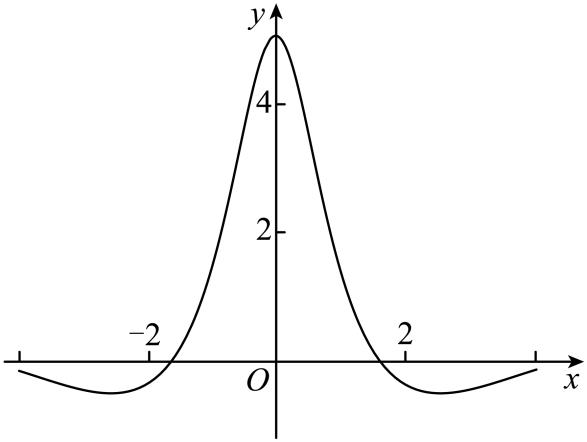
\includegraphics[width=.42\linewidth]{assets/asset-121-01.jpg}
\end{center}
\begin{choices}
  \item $\dfrac{5(e^x - e^{-x})}{x^2 + 2}$
  \item $\dfrac{5\sin x}{x^2 + 1}$
  \item $\dfrac{5(e^x + e^{-x})}{x^2 + 2}$
  \item $\dfrac{5\cos x}{x^2 + 1}$
\end{choices}
\begin{solution}
\textbf{答案：}D

\textbf{分析：}由图知函数为偶函数, 应用排除法.

\textbf{详解：}由图知: 函数图象关于 $y$ 轴对称, 其为偶函数, 且 $f(-2) = f(2) < 0$. 由 $\dfrac{5\sin(-x)}{(-x)^2 + 1} = -\dfrac{5\sin x}{x^2 + 1}$ 且定义域为 $\mathbb{R}$, 即 B 中函数为奇函数, 排除. 当 $x > 0$ 时 $\dfrac{5(e^x - e^{-x})}{x^2 + 2} > 0$, $\dfrac{5(e^x + e^{-x})}{x^2 + 2} > 0$, 即 A、C 中 $(0, +\infty)$ 上函数值为正, 排除. 故选 D.
\end{solution}
\end{question}

\begin{question}[points=5]
\textbf{来源：}2023 年 天津卷，第 15 题\par
若函数 $f(x) = |ax^2 - 2x| - |x^2 - ax + 1|$ 有且仅有两个零点，则 $a$ 的取值范围为．
\fillin[{$(-\infty, 0) \cup (0, 1) \cup (1, +\infty)$}]
\begin{solution}
\textbf{答案：}$(-\infty, 0) \cup (0, 1) \cup (1, +\infty)$

\textbf{分析：}分类讨论去掉绝对值，求出零点，再根据根存在的条件判断.

\textbf{详解：}当 $x^2 - ax + 1 \ge 0$ 时, $f(x)=0 \Leftrightarrow (a-1)x^2 + (a-2)x - 1 = 0$, 即 $[(a-1)x - 1](x+1)=0$. 若 $a=1$, 则 $x=-1$; 若 $a\neq1$, 则 $x = \frac{1}{a-1}$ 或 $x=-1$. 条件要求 $x^2 - ax + 1 \ge 0$ 成立, 对于 $x=-1$, 需 $1+a+1\ge0$ 即 $a\ge -2$; 对于 $x = \frac{1}{a-1}$, 需 $\frac{1}{(a-1)^2} - \frac{a}{a-1}+1 \ge 0$ 即 $a \le 2$ 且 $a\neq1$. 当 $x^2 - ax + 1 < 0$ 时, $f(x)=0 \Leftrightarrow (a+1)x^2 - (a+2)x + 1 = 0$, 即 $[(a+1)x - 1](x-1)=0$. 若 $a=-1$, 则 $x=1$ 不满足; 若 $a\neq -1$, 则 $x=1$ 或 $x = \frac{1}{a+1}$. 条件要求 $1 - a + 1 < 0$ 即 $a>2$ 对于 $x=1$, 对于 $x = \frac{1}{a+1}$ 需 $\frac{1}{(a+1)^2} - \frac{a}{a+1} + 1 < 0$ 即 $a<-2$. 综合所有情况, 当 $a<-2$, 零点为 $\frac{1}{a+1}$ 和 $\frac{1}{a-1}$; 当 $-2\le a<0$, 零点为 $\frac{1}{a-1}$ 和 $-1$; 当 $a=0$, 只有一个零点 $-1$; 当 $0<a<1$, 零点为 $\frac{1}{a-1}$ 和 $-1$; 当 $a=1$, 只有一个零点 $-1$; 当 $1<a\le2$, 零点为 $\frac{1}{a-1}$ 和 $-1$; 当 $a>2$, 零点为 $1$ 和 $-1$. 所以有两个零点时, $a\neq0$ 且 $a\neq1$, 即 $a \in (-\infty,0) \cup (0,1) \cup (1,+\infty)$.
\end{solution}
\end{question}

\begin{question}[points=5]
\textbf{来源：}2023 年 新高考II卷，第 4 题\par
若$f(x)=(x+a)\ln\dfrac{2x-1}{2x+1}$为偶函数，则$a=$（ \quad ）
\begin{choices}
  \item A. $-1$
  \item B. $0$
  \item C. $\dfrac{1}{2}$
  \item D. $1$
\end{choices}
\begin{solution}
\textbf{答案：}B

\textbf{分析：}根据偶函数性质，利用特殊值法求出$a$值，再检验即可.

\textbf{详解：}因为$f(x)$为偶函数，则$f(1)=f(-1)$，即$(1+a)\ln\dfrac{1}{3}=(-1+a)\ln3$，解得$a=0$；当$a=0$时，$f(x)=x\ln\dfrac{2x-1}{2x+1}$，定义域关于原点对称，且$f(-x)=(-x)\ln\dfrac{-2x-1}{-2x+1}=(-x)\ln\dfrac{2x+1}{2x-1}=x\ln\dfrac{2x-1}{2x+1}=f(x)$，故此时$f(x)$为偶函数.
\end{solution}
\end{question}

\begin{question}[points=5]
\textbf{来源：}2023 年 新高考I卷，第 4 题\par
设函数 $f(x)=2^{x(x-a)}$ 在区间 $(0,1)$ 上单调递减，则 $a$ 的取值范围是（ ）
\begin{choices}
  \item $(-\infty,-2]$
  \item $[-2,0)$
  \item $(0,2]$
  \item $[2,+\infty)$
\end{choices}
\begin{solution}
\textbf{答案：}$[2,+\infty)$

\textbf{分析：}利用指数型复合函数单调性，判断列式计算作答。

\textbf{详解：}函数 $y=2^x$ 在 $R$ 上单调递增，而函数 $f(x)=2^{x(x-a)}$ 在区间 $(0,1)$ 上单调递减，则有函数 $y=x(x-a)=(x-\frac{a}{2})^2-\frac{a^2}{4}$ 在区间 $(0,1)$ 上单调递减，因此 $\frac{a}{2}\geq 1$，解得 $a\geq 2$，所以 $a$ 的取值范围是 $[2,+\infty)$。
\end{solution}
\end{question}

\begin{question}[points=5]
\textbf{来源：}2023 年 新高考I卷，第 10 题\par
噪声污染问题越来越受到重视．用声压级来度量声音的强弱，定义声压级 $L_p=20\times\lg\frac{p}{p_0}$，其中常数 $p_0(p_0>0)$ 是听觉下限阈值，$p$ 是实际声压．下表为不同声源的声压级：



| 声源 | 与声源的距离 /m | 声压级 /dB |

|------|----------------|------------|

| 燃油汽车 | 10 | 60~90 |

| 混合动力汽车 | 10 | 50~60 |

| 电动汽车 | 10 | 40 |



已知在距离燃油汽车、混合动力汽车、电动汽车 10m 处测得实际声压分别为 $p_1, p_2, p_3$，则（ ）．
\begin{choices}
  \item $p_1\geq p_2$
  \item $p_2>10p_3$
  \item $p_3=100p_0$
  \item $p_1\leq 100p_2$
\end{choices}
\begin{solution}
\textbf{答案：}ACD

\textbf{分析：}根据题意可知 $L_{p_1}\in[60,90], L_{p_2}\in[50,60], L_{p_3}=40$，结合对数运算逐项分析判断。

\textbf{详解：}由题意可知：$L_{p_1}\in[60,90], L_{p_2}\in[50,60], L_{p_3}=40$。对于选项 A：$L_{p_1}-L_{p_2}=20\lg\frac{p_1}{p_0}-20\lg\frac{p_2}{p_0}=20\lg\frac{p_1}{p_2}$，因为 $L_{p_1}\geq L_{p_2}$，则 $L_{p_1}-L_{p_2}=20\lg\frac{p_1}{p_2}\geq 0$，即 $\lg\frac{p_1}{p_2}\geq 0$，所以 $\frac{p_1}{p_2}\geq 1$ 且 $p_1,p_2>0$，可得 $p_1\geq p_2$，故 A 正确。对于选项 B：$L_{p_2}-L_{p_3}=20\lg\frac{p_2}{p_0}-20\lg\frac{p_3}{p_0}=20\lg\frac{p_2}{p_3}$，因为 $L_{p_2}-L_{p_3}=L_{p_2}-40\geq 10$，则 $20\lg\frac{p_2}{p_3}\geq 10$，即 $\lg\frac{p_2}{p_3}\geq \frac{1}{2}$，所以 $\frac{p_2}{p_3}\geq e$ 且 $p_2,p_3>0$，可得 $p_2\geq e p_3$，当且仅当 $L_{p_2}=50$ 时，等号成立，故 B 错误。对于选项 C：因为 $L_{p_3}=20\lg\frac{p_3}{p_0}=40$，即 $\lg\frac{p_3}{p_0}=2$，可得 $\frac{p_3}{p_0}=100$，即 $p_3=100p_0$，故 C 正确。对于选项 D：由选项 A 可知：$L_{p_1}-L_{p_2}=20\lg\frac{p_1}{p_2}$，且 $L_{p_1}-L_{p_2}\leq 90-50=40$，则 $20\lg\frac{p_1}{p_2}\leq 40$，即 $\lg\frac{p_1}{p_2}\leq 2$，可得 $\frac{p_1}{p_2}\leq 100$，且 $p_1,p_2>0$，所以 $p_1\leq 100p_2$，故 D 正确。
\end{solution}
\end{question}

\begin{question}[points=5]
\textbf{来源：}2023 年 新高考I卷，第 11 题\par
已知函数 $f(x)$ 的定义域为 $\mathbb{R}$，$f(xy)=y^2f(x)+x^2f(y)$，则（ ）．
\begin{choices}
  \item $f(0)=0$
  \item $f(1)=0$
  \item $f(x)$ 是偶函数
  \item $x=0$ 为 $f(x)$ 的极小值点
\end{choices}
\begin{solution}
\textbf{答案：}ABC

\textbf{分析：}方法一：利用赋值法，结合函数奇偶性的判断方法可判断选项 ABC，举反例 $f(x)=0$ 即可排除选项 D。方法二：选项 ABC 的判断与方法一同，对于 D，可构造特殊函数 $f(x)=\begin{cases} x^2\ln|x|, & x\neq 0 \\ 0, & x=0 \end{cases}$ 进行判断即可。

\textbf{详解：}方法一：因为 $f(xy)=y^2f(x)+x^2f(y)$。对于 A，令 $x=y=0$，$f(0)=0\cdot f(0)+0\cdot f(0)=0$，故 A 正确。对于 B，令 $x=y=1$，$f(1)=1\cdot f(1)+1\cdot f(1)$，则 $f(1)=0$，故 B 正确。对于 C，令 $x=y=-1$，$f(1)=f(-1)+f(-1)=2f(-1)$，则 $f(-1)=0$，令 $y=-1$，$f(-x)=f(x)+x^2f(-1)=f(x)$，又函数 $f(x)$ 的定义域为 $\mathbb{R}$，所以 $f(x)$ 为偶函数，故 C 正确。对于 D，不妨令 $f(x)=0$，显然符合题设条件，此时 $f(x)$ 无极值，故 D 错误。方法二：对于 A、B、C 同方法一。对于 D，当 $x^2y^2\neq 0$ 时，对 $f(xy)=y^2f(x)+x^2f(y)$ 两边同时除以 $x^2y^2$，得到 $\frac{f(xy)}{x^2y^2}=\frac{f(x)}{x^2}+\frac{f(y)}{y^2}$，故可以设 $\frac{f(x)}{x^2}=\ln|x|(x\neq 0)$，则 $f(x)=\begin{cases} x^2\ln|x|, & x\neq 0 \\ 0, & x=0 \end{cases}$，当 $x>0$ 时，$f(x)=x^2\ln x$，则 $f'(x)=2x\ln x+x\cdot\frac{1}{x}=x(2\ln x+1)$，令 $f'(x)<0$，得 $0<x<e^{-\frac{1}{2}}$；令 $f'(x)>0$，得 $x>e^{-\frac{1}{2}}$，故 $f(x)$ 在 $(0,e^{-\frac{1}{2}})$ 上单调递减，在 $(e^{-\frac{1}{2}},+\infty)$ 上单调递增，因为 $f(x)$ 为偶函数，所以 $f(x)$ 在 $(-e^{-\frac{1}{2}},0)$ 上单调递增，在 $(-\infty,-e^{-\frac{1}{2}})$ 上单调递减，显然，此时 $x=0$ 是 $f(x)$ 的极大值，故 D 错误。
\end{solution}
\end{question}

\section*{2024 年}

\begin{question}[points=4]
\textbf{来源：}2024 年 北京卷，第 7 题\par
记水的质量为 $d=\dfrac{S-1}{\ln n}$，并且 $d$ 越大，水质量越好。若 $S$ 不变，且 $d_1=2.1$，$d_2=2.2$，则 $n_1$ 与 $n_2$ 的关系为（ ）
\begin{choices}
  \item $n_1 < n_2$
  \item $n_1 > n_2$
  \item 若 $S<1$，则 $n_1<n_2$；若 $S>1$，则 $n_1>n_2$；
  \item 若 $S<1$，则 $n_1>n_2$；若 $S>1$，则 $n_1<n_2$；
\end{choices}
\begin{solution}
\textbf{答案：}C

\textbf{分析：}根据题意分析可得 $\begin{cases} n_1 = e^{\frac{S-1}{2.1}} \\ n_2 = e^{\frac{S-1}{2.2}} \end{cases}$，讨论 $S$ 与 $1$ 的大小关系，结合指数函数单调性分析判断。

\textbf{详解：}由题意可得 $\begin{cases} d_1 = \dfrac{S-1}{\ln n_1}=2.1 \\ d_2 = \dfrac{S-1}{\ln n_2}=2.2 \end{cases}$，解得 $\begin{cases} n_1 = e^{\frac{S-1}{2.1}} \\ n_2 = e^{\frac{S-1}{2.2}} \end{cases}$。若 $S>1$，则 $\dfrac{S-1}{2.1} > \dfrac{S-1}{2.2}$，可得 $e^{\frac{S-1}{2.1}} > e^{\frac{S-1}{2.2}}$，即 $n_1>n_2$；若 $S=1$，则 $\dfrac{S-1}{2.1} = \dfrac{S-1}{2.2} =0$，可得 $n_1=n_2=1$；若 $S<1$，则 $\dfrac{S-1}{2.1} < \dfrac{S-1}{2.2}$，可得 $e^{\frac{S-1}{2.1}} < e^{\frac{S-1}{2.2}}$，即 $n_1<n_2$。结合选项可知 C 正确，ABD 错误。故选：C。
\end{solution}
\end{question}

\begin{question}[points=4]
\textbf{来源：}2024 年 北京卷，第 9 题\par
已知 $(x_1,y_1)$，$(x_2,y_2)$ 是函数 $y=2^x$ 图象上不同的两点，则下列正确的是（ ）
\begin{choices}
  \item $\log_2 \dfrac{y_1+y_2}{2} > \dfrac{x_1+x_2}{2}$
  \item $\log_2 \dfrac{y_1+y_2}{2} < \dfrac{x_1+x_2}{2}$
  \item $\log_2 \dfrac{y_1+y_2}{2} > x_1+x_2$
  \item $\log_2 \dfrac{y_1+y_2}{2} < x_1+x_2$
\end{choices}
\begin{solution}
\textbf{答案：}A

\textbf{分析：}根据指数函数和对数函数的单调性结合基本不等式分析判断AB；举例判断CD即可。

\textbf{详解：}由题意不妨设 $x_1<x_2$，因为函数 $y=2^x$ 是增函数，所以 $0<2^{x_1}<2^{x_2}$，即 $0<y_1<y_2$。对于选项AB：可得 $\dfrac{2^{x_1}+2^{x_2}}{2} > \sqrt{2^{x_1}\cdot2^{x_2}} = 2^{\frac{x_1+x_2}{2}}$，即 $\dfrac{y_1+y_2}{2} > 2^{\frac{x_1+x_2}{2}} > 0$，根据函数 $y=\log_2 x$ 是增函数，所以 $\log_2 \dfrac{y_1+y_2}{2} > \log_2 2^{\frac{x_1+x_2}{2}} = \dfrac{x_1+x_2}{2}$，故A正确，B错误。对于选项C：例如 $x_1=0, x_2=1$，则 $y_1=1, y_2=2$，可得 $\log_2 \dfrac{y_1+y_2}{2} = \log_2 \dfrac{3}{2} \in (0,1)$，即 $\log_2 \dfrac{y_1+y_2}{2} < 1 = x_1+x_2$，故C错误。对于选项D：例如 $x_1=-1, x_2=-2$，则 $y_1=\dfrac{1}{2}, y_2=\dfrac{1}{4}$，可得 $\log_2 \dfrac{y_1+y_2}{2} = \log_2 \dfrac{3}{8} = \log_2 3 - 3 \in (-2,-1)$，即 $\log_2 \dfrac{y_1+y_2}{2} > -3 = x_1+x_2$，故D错误。故选：A。
\end{solution}
\end{question}

\begin{question}[points=5]
\textbf{来源：}2024 年 全国甲卷-理科，第 7 题\par
函数 $f(x)=-x^2+(e^x-e^{-x})\sin x$ 在区间 $[-2.8,2.8]$ 的大致图像为（   ）

\begin{center}
  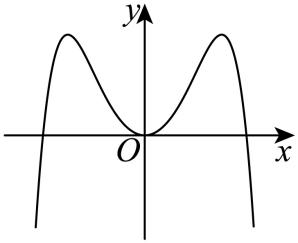
\includegraphics[width=.42\linewidth]{assets/asset-129-01.jpg}
\end{center}
\begin{choices}
  \item A
  \item B
  \item C
  \item D
\end{choices}
\begin{solution}
\textbf{答案：}B

\textbf{分析：}利用函数的奇偶性可排除 A、C，代入 $x=1$ 可得 $f(1)>0$，可排除 D。

\textbf{详解：}$f(-x)=-(-x)^2+(e^{-x}-e^x)\sin(-x)=-x^2+(e^x-e^{-x})\sin x=f(x)$，又函数定义域为 $[-2.8,2.8]$，故该函数为偶函数，可排除 A、C，又 $f(1)=-1+\left(e-\frac{1}{e}\right)\sin1>-1+\left(e-\frac{1}{e}\right)\sin\frac{\pi}{6}=\frac{e}{2}-1-\frac{1}{2e}>\frac{1}{4}-\frac{1}{2e}>0$，故可排除 D。
\end{solution}
\end{question}

\begin{question}[points=5]
\textbf{来源：}2024 年 全国甲卷-理科，第 15 题\par
已知 $a>1$，$\dfrac{1}{\log_8 a}-\dfrac{1}{\log_a 4}=-\dfrac{5}{2}$，则 $a=$ 。
\fillin[{$64$}]
\begin{solution}
\textbf{答案：}$64$

\textbf{分析：}将 $\log_8 a,\log_a 4$ 利用换底公式转化成 $\log_2 a$ 来表示即可求解。

\textbf{详解：}由题 $\frac{1}{\log_8 a}-\frac{1}{\log_a 4}=\frac{3}{\log_2 a}-\frac{1}{2}\log_2 a=-\frac{5}{2}$，整理得 $(\log_2 a)^2-5\log_2 a-6=0$，$\Rightarrow\log_2 a=-1$ 或 $\log_2 a=6$，又 $a>1$，所以 $\log_2 a=6=\log_2 2^6$，故 $a=2^6=64$。
\end{solution}
\end{question}

\begin{question}[points=5]
\textbf{来源：}2024 年 全国甲卷-文科，第 8 题\par
函数 $f(x) = -x^2 + (e^x - e^{-x})\sin x$ 在区间 $[-2.8, 2.8]$ 的大致图像为（ ）

\begin{center}
  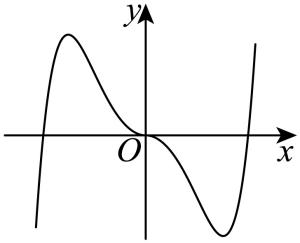
\includegraphics[width=.42\linewidth]{assets/asset-131-01.jpg}
\end{center}
\begin{choices}
  \item A
  \item B
  \item C
  \item D
\end{choices}
\begin{solution}
\textbf{答案：}B

\textbf{分析：}利用函数的奇偶性可排除A、C，代入 $x=1$ 可得 $f(1)>0$，可排除D.

\textbf{详解：}$f(-x) = -(-x)^2 + (e^{-x} - e^x)\sin(-x) = -x^2 + (e^x - e^{-x})\sin x = f(x)$，又函数定义域为 $[-2.8, 2.8]$，故该函数为偶函数，可排除A、C，又 $f(1) = -1 + (e - \frac{1}{e})\sin 1 > -1 + (e - \frac{1}{e})\sin \frac{\pi}{6} = -1 + \frac{e - 1/e}{2} > -\frac{1}{4} + \frac{1}{2e} > 0$，故可排除D.
\end{solution}
\end{question}

\begin{question}[points=5]
\textbf{来源：}2024 年 全国甲卷-文科，第 13 题\par
已知 $a > 1$，$\frac{1}{\log_8 a} - \frac{1}{\log_a 4} = -\frac{5}{2}$，则 $a =$ ．
\fillin[{$64$}]
\begin{solution}
\textbf{答案：}$64$

\textbf{分析：}将 $\log_8 a$，$\log_a 4$ 利用换底公式转化成 $\log_2 a$ 来表示即可求解.

\textbf{详解：}由题 $\frac{1}{\log_8 a} - \frac{1}{\log_a 4} = \frac{3}{\log_2 a} - \frac{1}{2}\log_2 a = -\frac{5}{2}$，整理得 $(\log_2 a)^2 - 5\log_2 a - 6 = 0$，$\Rightarrow \log_2 a = -1$ 或 $\log_2 a = 6$，又 $a > 1$，所以 $\log_2 a = 6 = \log_2 2^6$，故 $a = 2^6 = 64$.
\end{solution}
\end{question}

\begin{question}[points=5]
\textbf{来源：}2024 年 全国甲卷-文科，第 14 题\par
曲线 $y = x^3 - 3x$ 与 $y = -(x-1)^2 + a$ 在 $(0, +\infty)$ 上有两个不同的交点，则 $a$ 的取值范围为．
\fillin[{$(-2, 1)$}]
\begin{solution}
\textbf{答案：}$(-2, 1)$

\textbf{分析：}将函数转化为方程，令 $x^3 - 3x = -(x-1)^2 + a$，分离参数 $a$，构造新函数 $g(x) = x^3 + x^2 - 5x + 1$，结合导数求得 $g(x)$ 单调区间，画出大致图形数形结合即可求解.

\textbf{详解：}令 $x^3 - 3x = -(x-1)^2 + a$，即 $a = x^3 + x^2 - 5x + 1$，令 $g(x) = x^3 + x^2 - 5x + 1 \ (x > 0)$，则 $g'(x) = 3x^2 + 2x - 5 = (3x+5)(x-1)$，令 $g'(x) = 0 \ (x > 0)$ 得 $x = 1$，当 $x \in (0,1)$ 时，$g'(x) < 0$，$g(x)$ 单调递减，当 $x \in (1, +\infty)$ 时，$g'(x) > 0$，$g(x)$ 单调递增，$g(0) = 1$，$g(1) = -2$，因为曲线 $y = x^3 - 3x$ 与 $y = -(x-1)^2 + a$ 在 $(0, +\infty)$ 上有两个不同的交点，所以等价于 $y = a$ 与 $g(x)$ 有两个交点，所以 $a \in (-2, 1)$.
\end{solution}
\end{question}

\begin{question}[points=4]
\textbf{来源：}2024 年 上海卷，第 2 题\par
已知$f(x)=\begin{cases} \sqrt{x}, & x>0 \\ 1, & x\le 0 \end{cases}$，则$f(3)=$.
\fillin[{$3$}]
\begin{solution}
\textbf{答案：}$3$

\textbf{分析：}利用分段函数的形式可求$f(3)$.

\textbf{详解：}因为$f(x)=\begin{cases} \sqrt{x}, & x>0 \\ 1, & x\le 0 \end{cases}$，故$f(3)=\sqrt{3}=3$，故答案为：$3$.
\end{solution}
\end{question}

\begin{question}[points=4]
\textbf{来源：}2024 年 上海卷，第 4 题\par
已知$f(x)=x^3+a$，$x\in\mathbb{R}$，且$f(x)$是奇函数，则$a=$.
\fillin[{$0$}]
\begin{solution}
\textbf{答案：}$0$

\textbf{分析：}根据奇函数的性质可求参数$a$.

\textbf{详解：}因为$f(x)$是奇函数，故$f(-x)+f(x)=0$即$(-x)^3+a+x^3+a=0$，故$a=0$，故答案为：$0$.
\end{solution}
\end{question}

\begin{question}[points=5]
\textbf{来源：}2024 年 上海卷，第 16 题\par
已知函数$f(x)$的定义域为$\mathbb{R}$，定义集合$M=\{x_0\mid x_0\in\mathbb{R},\forall x\in(-\infty,x_0),f(x)<f(x_0)\}$，在使得$M=[-1,1]$的所有$f(x)$中，下列成立的是（\quad\quad）
\begin{choices}
  \item $A$存在$f(x)$是偶函数
  \item $B$存在$f(x)$在$x=2$处取最大值
  \item $C$存在$f(x)$是严格增函数
  \item $D$存在$f(x)$在$x=-1$处取到极小值
\end{choices}
\begin{solution}
\textbf{答案：}$B$

\textbf{分析：}对于ACD利用反证法并结合函数奇偶性、单调性以及极小值的概念即可判断，对于B，构造函数$f(x)=\begin{cases} -2, & x<-1 \\ x, & -1\le x\le1 \\ 1, & x>1 \end{cases}$即可判断.

\textbf{详解：}对于A，若存在$y=f(x)$是偶函数，取$x_0=1\in[-1,1]$，则对于任意$x\in(-\infty,1),f(x)<f(1)$，而$f(-1)=f(1)$，矛盾，故A错误；对于B，可构造函数$f(x)=\begin{cases} -2, & x<-1 \\ x, & -1\le x\le1 \\ 1, & x>1 \end{cases}$，满足集合$M=[-1,1]$，当$x<-1$时，则$f(x)=-2$，当$-1\le x\le1$时，$f(x)\in[-1,1]$，当$x>1$时，$f(x)=1$，则该函数$f(x)$的最大值是$f(2)$，则B正确；对C，假设存在$f(x)$，使得$f(x)$严格递增，则$M=\mathbb{R}$，与已知$M=[-1,1]$矛盾，则C错误；对D，假设存在$f(x)$，使得$f(x)$在$x=-1$处取极小值，则在-1的左侧附近存在$n$，使得$f(n)>f(-1)$，这与已知集合$M$的定义矛盾，故D错误；故选：B.
\end{solution}
\end{question}

\begin{question}[points=14]
\textbf{来源：}2024 年 上海卷，第 18 题\par
若$f(x)=\log_a x$（$a>0$a≠1）．
\begin{solution}
\textbf{答案：}（1）$\{x\mid1<x<2\}$；（2）$a>1$

\textbf{分析：}（1）求出底数$a$，再根据对数函数的单调性可求不等式的解；（2）存在$x$使得$f(x+1)$，$f(ax)$，$f(x+2)$成等差数列等价于$a^2=2\left(\frac1x+\frac34\right)^2-\frac18$在$(0,+\infty)$上有解，利用换元法结合二次函数的性质可求$a$的取值范围.

\textbf{详解：}（1）因为$y=f(x)$的图象过$(4,2)$，故$\log_a4=2$，故$a^2=4$即$a=2$（负的舍去），而$f(x)=\log_2x$在$(0,+\infty)$上为增函数，故$f(2x-2)<f(x)$，故$0<2x-2<x$即$1<x<2$，故$f(2x-2)<f(x)$的解集为$\{x\mid1<x<2\}$.（2）因为存在$x$使得$f(x+1)$，$f(ax)$，$f(x+2)$成等差数列，故$2f(ax)=f(x+1)+f(x+2)$有解，故$2\log_a(ax)=\log_a(x+1)+\log_a(x+2)$，因为$a>0$，$a\neq1$，故$x>0$，故$a^2x^2=(x+1)(x+2)$在$(0,+\infty)$上有解，由$a^2=\frac{x^2+3x+2}{x^2}=1+\frac3x+\frac2{x^2}=2\left(\frac1x+\frac34\right)^2-\frac18$在$(0,+\infty)$上有解，令$t=\frac1x\in(0,+\infty)$，而$y=2\left(t+\frac34\right)^2-\frac18$在$(0,+\infty)$上的值域为$(1,+\infty)$，故$a^2>1$即$a>1$.
\end{solution}
\end{question}

\begin{question}[points=5]
\textbf{来源：}2024 年 天津卷，第 4 题\par
下列函数是偶函数的是 ( )
\begin{choices}
  \item $y = \frac{e^x - x^2}{x^2 + 1}$
  \item $y = \frac{\cos x + x^2}{x^2 + 1}$
  \item $y = \frac{e^x - x}{x + 1}$
  \item $y = \frac{\sin x + 4x}{e^{|x|}}$
\end{choices}
\begin{solution}
\textbf{答案：}$y = \frac{\cos x + x^2}{x^2 + 1}$

\textbf{分析：}根据偶函数的判定方法一一判断即可.

\textbf{详解：}对 A, 设 $f(x)=\frac{e^x-x^2}{x^2+1}$, 定义域为 $\mathbb{R}$, 但 $f(-1)=\frac{e^{-1}-1}{2}$, $f(1)=\frac{e-1}{2}$, 则 $f(-1)\neq f(1)$, 故 A 错误. 对 B, 设 $g(x)=\frac{\cos x+x^2}{x^2+1}$, 定义域为 $\mathbb{R}$, 且 $g(-x)=\frac{\cos(-x)+(-x)^2}{(-x)^2+1}=\frac{\cos x+x^2}{x^2+1}=g(x)$, 则 $g(x)$ 为偶函数, 故 B 正确. 对 C, 设 $h(x)=\frac{e^x-x}{x+1}$, 定义域为 $\{x|x\neq -1\}$, 不关于原点对称, 则 $h(x)$ 不是偶函数, 故 C 错误. 对 D, 设 $\varphi(x)=\frac{\sin x+4x}{e^{|x|}}$, 定义域为 $\mathbb{R}$, 因为 $\varphi(1)=\frac{\sin 1+4}{e}$, $\varphi(-1)=\frac{-\sin 1-4}{e}$, 则 $\varphi(1)\neq\varphi(-1)$, 则 $\varphi(x)$ 不是偶函数, 故 D 错误. 故选 B.
\end{solution}
\end{question}

\begin{question}[points=5]
\textbf{来源：}2024 年 天津卷，第 5 题\par
若 $a = 4.2^{-0.3}$, $b = 4.2^{0.3}$, $c = \log_{4.2}{0.2}$, 则 $a$, $b$, $c$ 的大小关系为 ( )
\begin{choices}
  \item $a > b > c$
  \item $b > a > c$
  \item $c > a > b$
  \item $b > c > a$
\end{choices}
\begin{solution}
\textbf{答案：}$b > a > c$

\textbf{分析：}利用指数函数和对数函数的单调性分析判断即可.

\textbf{详解：}因为 $y=4.2^x$ 在 $\mathbb{R}$ 上递增, 且 $-0.3<0<0.3$, 所以 $0<4.2^{-0.3}<4.2^0<4.2^{0.3}$, 即 $0<a<1<b$. 因为 $y=\log_{4.2}x$ 在 $(0,+\infty)$ 上递增, 且 $0<0.2<1$, 所以 $\log_{4.2}{0.2}<\log_{4.2}{1}=0$, 即 $c<0$. 所以 $b>a>c$. 故选 B.
\end{solution}
\end{question}

\begin{question}[points=5]
\textbf{来源：}2024 年 天津卷，第 15 题\par
若函数 $f(x)=\sqrt{2x^2-ax} - |ax-2| + 1$ 有唯一零点, 则 $a$ 的取值范围为.
\fillin[{$(-\sqrt{3},-1)\cup(1,\sqrt{3})$}]
\begin{solution}
\textbf{答案：}$(-\sqrt{3},-1)\cup(1,\sqrt{3})$

\textbf{分析：}结合函数零点与两函数的交点的关系, 构造函数 $g(x)=\sqrt{2x^2-ax}$ 与 $h(x)=\begin{cases} ax-3, & x\geq\frac{2}{a} \\ 1-ax, & x<\frac{2}{a} \end{cases}$, 则两函数图象有唯一交点, 分 $a=0$、$a>0$ 与 $a<0$ 进行讨论.

\textbf{详解：}令 $f(x)=0$, 即 $\sqrt{2x^2-ax}=|ax-2|-1$. 由题 $x^2-ax\geq0$. 当 $a=0$ 时, $\sqrt{2x^2}=1$, $x=\pm\frac{\sqrt{2}}{2}$, 两解, 舍去. 当 $a>0$ 时, 则 $\sqrt{2x^2-ax}=|ax-2|-1=\begin{cases} ax-3, & x\geq\frac{2}{a}\\ 1-ax, & x<\frac{2}{a} \end{cases}$. 由 $x^2-ax\geq0$ 得 $x\geq a$ 或 $x\leq0$. 当 $x\leq0$ 时, $|ax-2|=2-ax$, 方程化为 $\sqrt{2x^2-ax}=1-ax$, 平方得 $(4-a^2)x^2-2ax-1=0$, 即 $[(2+a)x+1][(2-a)x-1]=0$. 当 $a=2$ 时, $4x+1=0$, $x=-\frac{1}{4}$; 当 $0<a<2$ 时, $x=-\frac{1}{2+a}$ 或 $x=\frac{1}{2-a}>0$ (舍); 当 $a>2$ 时, $x=-\frac{1}{2+a}<0$ 或 $x=\frac{1}{2-a}<0$, 两解, 舍去. 所以当 $0<a\leq2$ 时, 在 $x\leq0$ 时有唯一解. 则当 $0<a\leq2$ 时, 需在 $x\geq a$ 时无解. 当 $x\geq a$ 时, $h(x)=ax-3$, $g(x)=\sqrt{2x^2-ax}$, 令 $g(x)=0$ 得 $x=a$ (舍0). $g(x)$ 在 $(a,+\infty)$ 上单调递增. 要无交点, 则 $\frac{1}{a}<a$ 且 $\frac{3}{a}>a$, 解得 $1<a<\sqrt{3}$. 故 $1<a<\sqrt{3}$ 符合. 当 $a<0$ 时, 同理得 $-\sqrt{3}<a<-1$. 综上, $a\in(-\sqrt{3},-1)\cup(1,\sqrt{3})$.
\end{solution}
\end{question}

\begin{question}[points=5]
\textbf{来源：}2024 年 新高考II卷，第 6 题\par
设函数$f(x)=a(x+1)^2-1$，$g(x)=\cos x+2ax$，当$x\in(-1,1)$时，曲线$y=f(x)$与$y=g(x)$恰有一个交点，则$a=$（ ）
\begin{choices}
  \item $-1$
  \item $\dfrac{1}{2}$
  \item $1$
  \item $2$
\end{choices}
\begin{solution}
\textbf{答案：}$D$

\textbf{分析：}解法一：令$F(x)=ax^2+a-1$，$G(x)=\cos x$，分析可知曲线$y=F(x)$与$y=G(x)$恰有一个交点，结合偶函数的对称性可知该交点只能在$y$轴上，即可得$a=2$，并代入检验即可；解法二：令$h(x)=f(x)-g(x),x\in(-1,1)$，可知$h(x)$为偶函数，根据偶函数的对称性可知$h(x)$的零点只能为0，即可得$a=2$，并代入检验即可.

\textbf{详解：}解法一：令$f(x)=g(x)$，即$a(x+1)^2-1=\cos x+2ax$，可得$ax^2+a-1=\cos x$。令$F(x)=ax^2+a-1$，$G(x)=\cos x$。原题意等价于当$x\in(-1,1)$时，曲线$y=F(x)$与$y=G(x)$恰有一个交点。注意到$F(x),G(x)$均为偶函数，可知该交点只能在$y$轴上，可得$F(0)=G(0)$，即$a-1=1$，解得$a=2$。若$a=2$，令$F(x)=G(x)$，可得$2x^2+1-\cos x=0$。因为$x\in(-1,1)$，则$2x^2\ge0$，$1-\cos x\ge0$，当且仅当$x=0$时等号成立，可得$2x^2+1-\cos x\ge0$，当且仅当$x=0$时等号成立，则方程$2x^2+1-\cos x=0$有且仅有一个实根0，即曲线$y=F(x)$与$y=G(x)$恰有一个交点，所以$a=2$符合题意。综上所述：$a=2$。解法二：令$h(x)=f(x)-g(x)=ax^2+a-1-\cos x,x\in(-1,1)$，原题意等价于$h(x)$有且仅有一个零点。因为$h(-x)=a(-x)^2+a-1-\cos(-x)=ax^2+a-1-\cos x=h(x)$，则$h(x)$为偶函数，根据偶函数的对称性可知$h(x)$的零点只能为0，即$h(0)=a-2=0$，解得$a=2$。若$a=2$，则$h(x)=2x^2+1-\cos x,x\in(-1,1)$，又因为$2x^2\ge0$，$1-\cos x\ge0$当且仅当$x=0$时等号成立，可得$h(x)\ge0$，当且仅当$x=0$时等号成立，即$h(x)$有且仅有一个零点0，所以$a=2$符合题意.
\end{solution}
\end{question}

\begin{question}[points=5]
\textbf{来源：}2024 年 新高考II卷，第 8 题\par
设函数$f(x)=(x+a)\ln(x+b)$，若$f(x)\ge 0$，则$a^2+b^2$的最小值为（ ）
\begin{choices}
  \item $\dfrac{1}{8}$
  \item $\dfrac{1}{4}$
  \item $\dfrac{1}{2}$
  \item $1$
\end{choices}
\begin{solution}
\textbf{答案：}$C$

\textbf{分析：}解法一：由题意可知$f(x)$的定义域为$(-b,+\infty)$，分类讨论$-a$与$-b,1-b$的大小关系，结合符号分析判断，即可得$b=a+1$，代入可得最值；解法二：根据对数函数的性质分析$\ln(x+b)$的符号，进而可得$x+a$的符号，即可得$b=a+1$，代入可得最值.

\textbf{详解：}解法一：由题意可知$f(x)$的定义域为$(-b,+\infty)$。令$x+a=0$解得$x=-a$；令$\ln(x+b)=0$解得$x=1-b$。若$-a\le -b$，当$x\in(-b,1-b)$时，可知$x+a>0,\ln(x+b)<0$，此时$f(x)<0$，不合题意；若$-b<-a<1-b$，当$x\in(-a,1-b)$时，可知$x+a>0,\ln(x+b)<0$，此时$f(x)<0$，不合题意；若$-a=1-b$，当$x\in(-b,1-b)$时，可知$x+a<0,\ln(x+b)<0$，此时$f(x)>0$；当$x\in[1-b,+\infty)$时，可知$x+a\ge0,\ln(x+b)\ge0$，此时$f(x)\ge0$；可知若$-a=1-b$，符合题意；若$-a>1-b$，当$x\in(1-b,-a)$时，可知$x+a<0,\ln(x+b)>0$，此时$f(x)<0$，不合题意；综上所述：$-a=1-b$，即$b=a+1$，则$a^2+b^2=a^2+(a+1)^2=2\left(a+\dfrac{1}{2}\right)^2+\dfrac{1}{2}\ge\dfrac{1}{2}$，当且仅当$a=-\dfrac{1}{2},b=\dfrac{1}{2}$时等号成立，所以$a^2+b^2$的最小值为$\dfrac{1}{2}$。解法二：由题意可知$f(x)$的定义域为$(-b,+\infty)$。令$x+a=0$解得$x=-a$；令$\ln(x+b)=0$解得$x=1-b$。则当$x\in(-b,1-b)$时，$\ln(x+b)<0$，故$x+a\le0$，所以$1-b+a\le0$；$x\in(1-b,+\infty)$时，$\ln(x+b)>0$，故$x+a\ge0$，所以$1-b+a\ge0$；故$1-b+a=0$，则$a^2+b^2=a^2+(a+1)^2=2\left(a+\dfrac{1}{2}\right)^2+\dfrac{1}{2}\ge\dfrac{1}{2}$，当且仅当$a=-\dfrac{1}{2},b=\dfrac{1}{2}$时等号成立，所以$a^2+b^2$的最小值为$\dfrac{1}{2}$.
\end{solution}
\end{question}

\begin{question}[points=6]
\textbf{来源：}2024 年 新高考II卷，第 11 题；次专题：导数\par
设函数$f(x)=2x^3-3ax^2+1$，则（ ）
\begin{choices}
  \item 当$a>1$时，$f(x)$有三个零点
  \item 当$a<0$时，$x=0$是$f(x)$的极大值点
  \item 存在$a,b$，使得$x=b$为曲线$y=f(x)$的对称轴
  \item 存在$a$，使得点$(1,f(1))$为曲线$y=f(x)$的对称中心
\end{choices}
\begin{solution}
\textbf{答案：}$AD$

\textbf{分析：}A选项，先分析出函数的极值点为$x=0,x=a$，根据零点存在定理和极值的符号判断出$f(x)$在$(-1,0),(0,a),(a,2a)$上各有一个零点；B选项，根据极值和导函数符号的关系进行分析；C选项，假设存在这样的$a,b$，使得$x=b$为$f(x)$的对称轴，则$f(x)=f(2b-x)$为恒等式，据此计算判断；D选项，若存在这样的$a$，使得$(1,3-3a)$为$f(x)$的对称中心，则$f(x)+f(2-x)=6-6a$，据此进行计算判断，亦可利用拐点结论直接求解.

\textbf{详解：}A选项，$f'(x)=6x^2-6ax=6x(x-a)$，由于$a>1$，故$x\in(-\infty,0)\cup(a,+\infty)$时$f'(x)>0$，故$f(x)$在$(-\infty,0),(a,+\infty)$上单调递增，$x\in(0,a)$时$f'(x)<0$，$f(x)$单调递减，则$f(x)$在$x=0$处取到极大值，在$x=a$处取到极小值。由$f(0)=1>0$，$f(a)=1-a^3<0$，则$f(0)f(a)<0$，根据零点存在定理$f(x)$在$(0,a)$上有一个零点；又$f(-1)=-1-3a<0$，$f(2a)=4a^3+1>0$，则$f(-1)f(0)<0$，$f(a)f(2a)<0$，则$f(x)$在$(-1,0),(a,2a)$上各有一个零点，于是$a>1$时，$f(x)$有三个零点，A选项正确。B选项，$f'(x)=6x(x-a)$，$a<0$时，$x\in(a,0)$时$f'(x)<0$，$f(x)$单调递减，$x\in(0,+\infty)$时$f'(x)>0$，$f(x)$单调递增，此时$f(x)$在$x=0$处取到极小值，B选项错误。C选项，假设存在这样的$a,b$，使得$x=b$为$f(x)$的对称轴，即存在这样的$a,b$使得$f(x)=f(2b-x)$，即$2x^3-3ax^2+1=2(2b-x)^3-3a(2b-x)^2+1$，根据二项式定理，等式右边$(2b-x)^3$展开式含有$x^3$的项为$2C_3^0(2b)^3(-x)^3=-2x^3$，于是等式左右两边$x^3$的系数不相等，原等式不可能恒成立，于是不存在这样的$a,b$，使得$x=b$为$f(x)$的对称轴，C选项错误。D选项，方法一：利用对称中心的表达式化简。$f(1)=3-3a$，若存在这样的$a$，使得$(1,3-3a)$为$f(x)$的对称中心，则$f(x)+f(2-x)=6-6a$。事实上，$f(x)+f(2-x)=2x^3-3ax^2+1+2(2-x)^3-3a(2-x)^2+1=(12-6a)x^2+(12a-24)x+18-12a$，于是$6-6a=(12-6a)x^2+(12a-24)x+18-12a$，即$\begin{cases}12-6a=0\\12a-24=0\\18-12a=6-6a\end{cases}$，解得$a=2$，即存在$a=2$使得$(1,f(1))$是$f(x)$的对称中心，D选项正确。方法二：直接利用拐点结论。任何三次函数都有对称中心，对称中心的横坐标是二阶导数的零点。$f(x)=2x^3-3ax^2+1$，$f'(x)=6x^2-6ax$，$f''(x)=12x-6a$，由$f''(x)=0\Leftrightarrow x=\dfrac{a}{2}$，于是该三次函数的对称中心为$\left(\dfrac{a}{2},f\left(\dfrac{a}{2}\right)\right)$。由题意$(1,f(1))$也是对称中心，故$\dfrac{a}{2}=1\Leftrightarrow a=2$，即存在$a=2$使得$(1,f(1))$是$f(x)$的对称中心，D选项正确。
\end{solution}
\end{question}

\begin{question}[points=5]
\textbf{来源：}2024 年 新高考I卷，第 6 题\par
已知函数 $f(x)=\begin{cases}-x^2-2ax-a, & x<0 \\ e^x+\ln(x+1), & x\ge 0\end{cases}$ 在 $\mathbb{R}$ 上单调递增，则 $a$ 的取值范围是（ ）
\begin{choices}
  \item $(-\infty,0]$
  \item $[-1,0]$
  \item $[-1,1]$
  \item $[0,+\infty)$
\end{choices}
\begin{solution}
\textbf{答案：}B

\textbf{分析：}根据二次函数的性质和分界点的大小关系即可得到不等式组，解出即可.

\textbf{详解：}因为 $f(x)$ 在 $\mathbb{R}$ 上单调递增，且 $x\ge 0$ 时，$f(x)=e^x+\ln(x+1)$ 单调递增，则需满足 $\begin{cases} -\dfrac{-2a}{2\times(-1)}\ge 0 \\ -a\le e^0+\ln1 \end{cases}$，解得 $-1\le a\le 0$，即 $a$ 的范围是 $[-1,0]$.
\end{solution}
\end{question}

\begin{question}[points=5]
\textbf{来源：}2024 年 新高考I卷，第 8 题；次专题：数列\par
已知函数 $f(x)$ 的定义域为 $\mathbb{R}$，$f(x)>f(x-1)+f(x-2)$，且当 $x<3$ 时 $f(x)=x$，则下列结论中一定正确的是（ ）
\begin{choices}
  \item $f(10)>100$
  \item $f(20)>1000$
  \item $f(10)<1000$
  \item $f(20)<10000$
\end{choices}
\begin{solution}
\textbf{答案：}B

\textbf{分析：}代入得到 $f(1)=1,f(2)=2$，再利用函数性质和不等式的性质，逐渐递推即可判断.

\textbf{详解：}因为当 $x<3$ 时 $f(x)=x$，所以 $f(1)=1,f(2)=2$，又因为 $f(x)>f(x-1)+f(x-2)$，则 $f(3)>f(2)+f(1)=3$, $f(4)>5$, $f(5)>8$, $f(6)>13$, $f(7)>21$, $f(8)>34$, $f(9)>55$, $f(10)>89$, $f(11)>144$, $f(12)>233$, $f(13)>377$, $f(14)>610$, $f(15)>987$, $f(16)>1597>1000$，则依次下去可知 $f(20)>1000$，则 B 正确；且无证据表明 ACD 一定正确.
\end{solution}
\end{question}

\begin{question}[points=6]
\textbf{来源：}2024 年 新高考I卷，第 10 题；次专题：导数\par
设函数 $f(x)=(x-1)^2(x-4)$，则（ ）
\begin{choices}
  \item $x=3$ 是 $f(x)$ 的极小值点
  \item 当 $0<x<1$ 时，$f(x)<f(x^2)$
  \item 当 $1<x<2$ 时，$-4<f(2x-1)<0$
  \item 当 $-1<x<0$ 时，$f(2-x)>f(x)$
\end{choices}
\begin{solution}
\textbf{答案：}ACD

\textbf{分析：}求出函数 $f(x)$ 的导数，得到极值点，即可判断 A；利用函数的单调性可判断 B；根据函数 $f(x)$ 在 $(1,3)$ 上的值域即可判断 C；直接作差可判断 D.

\textbf{详解：}对 A，因为 $f'(x)=2(x-1)(x-4)+(x-1)^2=3(x-1)(x-3)$，易知当 $x\in(1,3)$ 时 $f'(x)<0$，当 $x\in(-\infty,1)$ 或 $x\in(3,+\infty)$ 时 $f'(x)>0$，函数 $f(x)$ 在 $(-\infty,1)$ 上单调递增，在 $(1,3)$ 上单调递减，在 $(3,+\infty)$ 上单调递增，故 $x=3$ 是函数 $f(x)$ 的极小值点，正确；对 B，当 $0<x<1$ 时，$x-x^2=x(1-x)>0$，所以 $1>x>x^2>0$，而由上可知，函数 $f(x)$ 在 $(0,1)$ 上单调递增，所以 $f(x)>f(x^2)$，错误；对 C，当 $1<x<2$ 时，$1<2x-1<3$，而函数 $f(x)$ 在 $(1,3)$ 上单调递减，所以 $f(1)>f(2x-1)>f(3)$，即 $-4<f(2x-1)<0$，正确；对 D，当 $-1<x<0$ 时，$f(2-x)-f(x)=(1-x)^2(-2-x)-(x-1)^2(x-4)=(x-1)^2(2-2x)>0$，所以 $f(2-x)>f(x)$，正确.
\end{solution}
\end{question}

\section*{2025 年}

\begin{question}[points=6]
\textbf{来源：}2025 年 全国II卷，第 10 题\par
已知 $f(x)$ 是定义在 $\mathbb{R}$ 上的奇函数，且当 $x>0$ 时，$f(x)=(x^2-3)e^x+2$，则（ ）
\begin{choices}
  \item $f(0)=0$
  \item 当 $x<0$ 时，$f(x)=-(x^2-3)e^{-x}-2$
  \item $f(x)\ge 2$ 当且仅当 $x\ge\sqrt{3}$
  \item $x=-1$ 是 $f(x)$ 的极大值点
\end{choices}
\begin{solution}
\textbf{答案：}$ABD$

\textbf{分析：}对A，根据奇函数特点即可判断；对B，利用 $f(x)=-f(-x)$ 代入求解即可；对C，举反例 $f(-1)>2$ 即可；对D，直接求导，根据极大值点判定方法即可判断.

\textbf{详解：}对A，因为 $f(x)$ 是定义在 $\mathbb{R}$ 上的奇函数，则 $f(0)=0$，故A正确；对B，当 $x<0$ 时，$-x>0$，则 $f(x)=-f(-x)=-[(-x)^2-3]e^{-x}-2=-(x^2-3)e^{-x}-2$，故B正确；对C，$f(-1)=-(1-3)e^{-1}-2=2e^{-1}-2<0$，故C错误；对D，当 $x<0$ 时，$f(x)=-(x^2-3)e^{-x}-2$，则 $f'(x)=-(2x)e^{-x}+(x^2-3)e^{-x}=(x^2-2x-3)e^{-x}$，令 $f'(x)=0$，解得 $x=-1$ 或 $x=3$（舍去），当 $x\in(-\infty,-1)$ 时，$f'(x)>0$，$f(x)$ 单调递增；当 $x\in(-1,0)$ 时，$f'(x)<0$，$f(x)$ 单调递减，则 $x=-1$ 是 $f(x)$ 的极大值点，故D正确.
\end{solution}
\end{question}

\begin{question}[points=5]
\textbf{来源：}2025 年 全国II卷，第 13 题；次专题：导数\par
若 $x=2$ 是函数 $f(x)=(x-1)(x-2)(x-a)$ 的极值点，则 $f(0)=$.
\fillin[{$-4$}]
\begin{solution}
\textbf{答案：}$-4$

\textbf{分析：}由题意得 $f'(2)=0$ 即可求解 $a$，再代入即可求解.

\textbf{详解：}由题意有 $f(x)=(x-1)(x-2)(x-a)$，所以 $f'(x)=(x-a)(x-1)+(x-1)(x-2)+(x-a)(x-2)$，因为 $2$ 是函数 $f(x)$ 的极值点，所以 $f'(2)=2-a=0$，得 $a=2$. 当 $a=2$ 时，$f'(x)=2(x-2)(x-1)+(x-2)^2=(x-2)(3x-4)$，当 $x\in(-\infty,\frac{4}{3})$ 时 $f'(x)>0$，$f(x)$ 单调递增；当 $x\in(\frac{4}{3},2)$ 时 $f'(x)<0$，$f(x)$ 单调递减；当 $x\in(2,+\infty)$ 时 $f'(x)>0$，$f(x)$ 单调递增，所以 $x=2$ 是函数 $f(x)=(x-1)(x-2)(x-a)$ 的极小值点，符合题意；所以 $f(0)=(-1)\times(-2)\times(-a)=-2a=-4$.
\end{solution}
\end{question}

\begin{question}[points=5]
\textbf{来源：}2025 年 全国I卷，第 5 题\par
设 $f(x)$ 是定义在 $\mathbb{R}$ 上且周期为 $2$ 的偶函数，当 $2 \le x \le 3$ 时，$f(x)=5-2x$，则 $f\left(-\frac{3}{4}\right)=$（ ）
\begin{choices}
  \item $-\frac{1}{2}$
  \item $-\frac{1}{4}$
  \item $\frac{1}{4}$
  \item $\frac{1}{2}$
\end{choices}
\begin{solution}
\textbf{答案：}A

\textbf{分析：}根据周期性和奇偶性把待求自变量转化为 $[2,3]$ 的范围中求解.

\textbf{详解：}由题知 $f(x)=f(-x), f(x+2)=f(x)$ 对一切 $x \in \mathbb{R}$ 成立，于是 $f\left(-\frac{3}{4}\right) = f\left(\frac{3}{4}\right) = f\left(\frac{11}{4}\right) = 5 - 2\times\frac{11}{4} = -\frac{1}{2}$. 故选：A.
\end{solution}
\end{question}

\begin{question}[points=5]
\textbf{来源：}2025 年 全国I卷，第 8 题\par
若实数 $x$，$y$，$z$ 满足 $2 + \log_2 x = 3 + \log_3 y = 5 + \log_5 z$，则 $x$，$y$，$z$ 的大小关系不可能是（ ）
\begin{choices}
  \item $x > y > z$
  \item $x > z > y$
  \item $y > x > z$
  \item $y > z > x$
\end{choices}
\begin{solution}
\textbf{答案：}B

\textbf{分析：}法一：设 $2+\log_2 x = 3+\log_3 y = 5+\log_5 z = m$，对 $m$ 讨论赋值求出 $x,y,z$，即可得出大小关系，利用排除法求出；法二：根据数形结合解出.

\textbf{详解：}法一：设 $2+\log_2 x = 3+\log_3 y = 5+\log_5 z = m$，令 $m=2$，则 $x=1,y=3^{-1}=\frac{1}{3},z=5^{-3}=\frac{1}{125}$，此时 $x>y>z$，A 有可能；令 $m=5$，则 $x=8,y=9,z=1$，此时 $y>x>z$，C 有可能；令 $m=8$，则 $x=2^6=64,y=3^5=243,z=5^3=125$，此时 $y>z>x$，D 有可能；故选：B．法二：设 $2+\log_2 x = 3+\log_3 y = 5+\log_5 z = m$，所以 $x=2^{m-2}, y=3^{m-3}, z=5^{m-5}$，作出函数 $y=2^{x-2}, y=3^{x-3}, y=5^{x-5}$ 的图象，易知随着 $m$ 的变化可能出现：$x>y>z$，$y>x>z$，$y>z>x$，$z>y>x$，故选：B.
\end{solution}
\end{question}

\begin{question}[points=4]
\textbf{来源：}2025 年 上海卷，第 14 题；次专题：集合与逻辑\par
设 $a > 0, s \in \mathbf{R}$．下列各项中，能推出 $a^s > a$ 的一项是（ ）
\begin{choices}
  \item $a > 1$，且 $s > 0$
  \item $a > 1$，且 $s < 0$
  \item $0 < a < 1$，且 $s > 0$
  \item $0 < a < 1$，且 $s < 0$
\end{choices}
\begin{solution}
\textbf{答案：}D

\textbf{分析：}利用指数函数的性质分类讨论 $a$ 与 $1$ 的关系即可判定选项.

\textbf{详解：}$\because a > 0, a^s > a$，$\therefore a^{s-1} > 1 = a^0$，当 $a \in (0,1)$ 时，$y = a^x$ 定义域上严格单调递减，此时若 $s-1 < 0$，则一定有 $a^{s-1} > 1 = a^0$ 成立，故 D 正确，C 错误；当 $a \in (1, +\infty)$ 时，$y = a^x$ 定义域上严格单调递增，要满足 $a^{s-1} > 1 = a^0$，需 $s > 1$，即 A、B 错误. 故选：D.
\end{solution}
\end{question}

\begin{question}[points=18]
\textbf{来源：}2025 年 上海卷，第 21 题；次专题：三角函数\par
已知函数 $y = f(x)$ 的定义域为 $\mathbf{R}$．对于正实数 $a$，定义集合 $M_a = \{x \mid f(x+a) = f(x)\}$．

(1) 若 $f(x) = \sin x$，判断 $\frac{\pi}{3}$ 是否是 $M_\pi$ 中的元素，请说明理由；

(2) 若 $f(x) = \begin{cases} x+2, & x < 0 \\ x, & x \geq 0 \end{cases}$，$M_a \neq \varnothing$，求 $a$ 的取值范围；

(3) 若 $y = f(x)$ 是偶函数，当 $x \in (0,1]$ 时，$f(x) = 1 - x$，且对任意 $a \in (0,2)$，均有 $M_a \subseteq M_2$．写出 $y = f(x)$，$x \in (1,2)$ 解析式，并证明：对任意实数 $c$，函数 $y = f(x) - c$ 在 $[-3,3]$ 上至多有 $9$ 个零点．
\begin{solution}
\textbf{答案：}(1) 不是； (2) $\left[\frac{7}{4}, 4\right)$； (3) 解析式 $f(x) = x - 1, x \in (1,2)$；证明见解析

\textbf{分析：}(1) 直接代入计算 $f\left(\frac{\pi}{3}\right)$ 和 $f\left(\frac{\pi}{3} + \pi\right)$ 即可； (2) 法一：转化为存在实数 $x_0$ 使得 $f(x_0 + a) = f(x_0)$，分析得 $x_0 + 2 = \sqrt{x_0 + a}$，再计算得 $a = (x_0 + 2)^2 - x_0 = \left(x_0 + \frac{3}{2}\right)^2 + \frac{7}{4}$，最后根据 $x_0$ 的范围即可得到答案；法二：画出函数图象，转化为直线 $y = t$ 与该函数有两个交点，将 $a$ 用 $t$ 表示，最后利用二次函数性质即可得到答案； (3) 利用函数奇偶性和集合新定义即可求出 $x \in (1,2)$ 时解析式，再分析出 $f(-3) \notin (0,1)$，最后对 $c$ 的范围进行分类讨论即可.

\textbf{详解：}(1) $f\left(\frac{\pi}{3}\right) = \sin\frac{\pi}{3} = \frac{\sqrt{3}}{2}$，$f\left(\frac{\pi}{3} + \pi\right) = -\sin\frac{\pi}{3} = -\frac{\sqrt{3}}{2}$，两者不相等，故 $\frac{\pi}{3}$ 不是 $M_\pi$ 中的元素．
(2) 法一：因为 $M_a \neq \varnothing$，则存在实数 $x_0$ 使得 $f(x_0 + a) = f(x_0)$，且 $a > 0$，当 $x < 0$ 时，$f(x) = x+2$，其在 $(-\infty, 0)$ 上严格单调递增，当 $x \geq 0$ 时，$f(x) = \sqrt{x}$，其在 $[0, +\infty)$ 上也严格单调递增，则 $x_0 < 0 \leq x_0 + a$，则 $x_0 + 2 = \sqrt{x_0 + a}$，令 $x+2 = 0$，解得 $x = -2$，则 $-2 \leq x_0 < 0$，则 $a = (x_0 + 2)^2 - x_0 = \left(x_0 + \frac{3}{2}\right)^2 + \frac{7}{4} \in \left[\frac{7}{4}, 4\right)$．法二：作出该函数图象，则由题意知直线 $y = t$ 与该函数有两个交点，由图知 $0 \leq t < 2$，假设交点分别为 $A(m, t)$，$B(n, t)$，联立方程组 $\begin{cases} m = t^2 \\ n+2 = t \end{cases}$ 得 $a = |AB| = m - n = t^2 - (t-2) = \left(t - \frac{1}{2}\right)^2 + \frac{7}{4} \in \left[\frac{7}{4}, 4\right)$．
(3) 对任意 $x_0 \in (1,2)$，$x_0 - 2 \in (-1,0)$，因为其是偶函数，则 $f(x_0 - 2) = f(2 - x_0)$，而 $4 - 2x_0 \in (0,2)$，所以 $x_0 - 2 \in M_{4-2x_0} \subseteq M_2$，所以 $f(x_0) = f(x_0 - 2) = f(2 - x_0)$，因为 $x_0 \in (1,2)$，则 $2 - x_0 \in (0,1)$，所以 $f(x_0) = f(2 - x_0) = 1 - (2 - x_0) = x_0 - 1$，所以 $f(x) = x - 1, x \in (1,2)$．所以当 $s \in (0,1)$ 时，$1-s \in (0,1)$，$1+s \in (1,2)$，则 $f(1-s) = 1 - (1-s) = s$，$f(1+s) = (1+s) - 1 = s$，则 $f(1-s) = f(1+s)$，而 $1+s - (1-s) = 2s$，$(3-s) - (1-s) = 2$，则 $1-s \in M_{2s} \subseteq M_2$，则 $f(1-s) = f(3-s)$，所以当 $x \in (2,3)$ 时，$f(x) = f(x-2) = 1 - (x-2) = 3 - x$，而 $f(x)$ 为偶函数，画出函数图象如下：其中 $f(-3) = f(3)$，$f(-2) = f(2)$，$f(0)$，但其对应的 $y$ 值均未知．首先说明 $f(-3) = n \notin (0,1)$，若 $f(-3) = n \in (0,1)$，则 $-3+n \in (-3,-2)$，易知此时 $f(x) = x+3, x \in (-3,-2)$，则 $f(-3+n) = n$，所以 $f(-3) \in M_n \subseteq M_2$，而 $x \in [-1,0)$ 时，$f(x) = x+1$，所以 $f(-3) = f(-1) = 0$，与 $f(-3) = n$ 矛盾，所以 $f(-3) \notin (0,1)$，即 $f(-3) = f(3) \notin (0,1)$．令 $y = f(x) - c = 0$，则 $y = f(x) = c$，当 $c = 0$ 时，即使让 $f(-3) = f(3) = f(-2) = f(2) = f(0) = 0$，此时最多 $7$ 个零点；当 $c \geq 1$ 时，若 $f(-2) = f(2) = f(0) = f(-3) = f(3) = c$，此时有 $5$ 个零点，故此时最多 $5$ 个零点；当 $c < 0$ 时，若 $f(-2) = f(2) = f(0) = f(-3) = f(3) = c$，此时有 $5$ 个零点，故此时最多 $5$ 个零点；当 $0 < c < 1$ 时，若 $f(-2) = f(2) = f(0) = c$，此时有 $3$ 个零点，若 $f(-3) = c \in (0,1)$，则 $-3+c \in (-3,-2)$，易知此时 $f(x) = x+3$，则 $f(-3+c) = c$，所以 $f(-3) \in M_c \subseteq M_2$，而 $x \in [-1,0)$ 时，$f(x) = x+1$，所以 $f(-3) = f(-1) = 0$，与 $f(-3) = c$ 矛盾，所以 $f(-3) \notin (0,1)$，则最多在 $(-3,-2), (-2,-1), (-1,0), (0,1), (1,2), (2,3)$ 之间取得 $6$ 个零点，以及在 $x = -2, 0, 2$ 处成为零点，故不超过 $9$ 个零点．综上，零点不超过 $9$ 个.
\end{solution}
\end{question}

\begin{question}[points=5]
\textbf{来源：}2025 年 天津卷，第 3 题\par
已知函数$y = f(x)$的图象如下, 则$f(x)$的解析式可能为（   ）
\begin{choices}
  \item $f(x) = \dfrac{x}{1 - |x|}$
  \item $f(x) = \dfrac{x}{|x| - 1}$
  \item $f(x) = \dfrac{|x|}{1 - x^2}$
  \item $f(x) = \dfrac{|x|}{x^2 - 1}$
\end{choices}
\begin{solution}
\textbf{答案：}D

\textbf{分析：}先由函数奇偶性排除AB，再由$x \in (0,1)$时函数值正负情况可得解.

\textbf{详解：}由图可知函数为偶函数，而函数$f(x) = \dfrac{x}{1-x}$和函数$f(x) = \dfrac{x}{x-1}$为奇函数，故排除选项AB；又当$x \in (0,1)$时$1 - x^2 > 0$, $x^2 - 1 < 0$, 此时$f(x) = \dfrac{x}{1-x^2} > 0$, $f(x) = \dfrac{x}{x^2-1} < 0$, 由图可知当$x \in (0,1)$时, $f(x) < 0$, 故C不符合，D符合. 故选D.
\end{solution}
\end{question}

\begin{question}[points=5]
\textbf{来源：}2025 年 天津卷，第 7 题\par
函数$f(x) = 0.3^x - \sqrt{x}$的零点所在区间是（   ）
\begin{choices}
  \item $(0, 0.3)$
  \item $(0.3, 0.5)$
  \item $(0.5, 1)$
  \item $(1, 2)$
\end{choices}
\begin{solution}
\textbf{答案：}B

\textbf{分析：}利用指数函数与幂函数的单调性结合零点存在性定理计算即可.

\textbf{详解：}由指数函数、幂函数的单调性可知：$y = 0.3^x$在$\mathbb{R}$上单调递减, $y = \sqrt{x}$在$[0, +\infty)$单调递增, 所以$f(x) = 0.3^x - \sqrt{x}$在定义域上单调递减. 显然$f(0) = 1 > 0$, $f(0.3) = 0.3^{0.3} - \sqrt{0.3} > 0$, $f(0.5) = 0.3^{0.5} - \sqrt{0.5} < 0$, 所以根据零点存在性定理可知$f(x)$的零点位于$(0.3, 0.5)$. 故选B.
\end{solution}
\end{question}

